% !TeX encoding = UTF-8
%% \textbf{重庆大学}通用毕业论文\LaTeXe{}模板
%%% 使用前请先阅读使用文档和用户协议,内有详细介绍。Happy Texing! :)
%% =======================================================
\documentclass%
	[type=master, bilinguallist=apart, 
	printmode=oneside, blindtrail=false, proffesionalmaster=true]{cquthesis}%
% 可用选项:
% type=[bachelor|master|doctor],      % 必选,毕业论文类型,以下项目不填时为默认
% liberalformat,                      % 可选,仅适用本科生,使用文学类论文标题格式,默认未打开
% proffesionalmaster=[true|false],    % 可选,仅适用研究生,是(true)否(false)专业硕士,默认为否
% printmode=[oneside|twoside|auto],	  % 可选,论文打印方式,默认采用auto按页数要求自动判定
% openany,|openright,                 % 可选,双面打印时每章的第一页仅右页开启,默认右页开启(openright)
% bilinguallist=[off|combined|apart], % 可选,图录表录等分别按双语题注混编(combined),分开编录(apart),默认关(off)
% blindtrail=[true|false],                         % 可选,盲审模式,开启后封面姓名和致谢部分会隐藏,详情请参阅用户文档,默认关
% draft,                              % 写作期间可选,不渲染图片,关闭外围功能,加快预览速度,默认未开启

% 请在cquthesis.sty文件中定义其他会用到的宏包和自己的变量
% 这样可以防止main.tex太过臃肿。
\usepackage{cquthesis}

% 定义所有的图片文件在 figures 子目录下
\graphicspath{{figures/}}

% 定义数字圆
\usepackage{tikz}
\newcommand*\circled[1]{\tikz[baseline=(char.base)]{
            \node[shape=circle,draw,inner sep=1pt] (char) {\small #1};}}

%*** 写作时,使用这个命令只渲染你想查看的部分,提升工作效率,定稿时注释掉整行
% \includeonly{contents/introduction}
% \includeonly{contents/related_work}
%\includeonly{contents/CRMMIL}
% \includeonly{contents/SMCMIL}
 


\begin{document}


\cqusetup{
%	************	注意	************
%	* 1. \cqusetup{}中不能出现全空的行,如果需要全空行请在行首注释
%	* 2. 不需要的配置信息可以放心地坐视不理、留空、删除或注释(都不会有影响)
%	*
%	********************************
% ===================
%	论文的中英文题目
% ===================
  ctitle = {基于Mamba的高分辨率病理图像分类算法研究},
  etitle = {Research on High-Resolution Medical Pathology WSI Image Classification Algorithm Based on Mamba},
% ===================
% 作者部分的信息
% \secretize{}为盲审标记点,在打开盲审开关时内容会自动被替换为***输出,盲审开关默认关闭
% ===================
  cauthor = \secretize{朱翔},	% 你的姓名,以下每项都以英文逗号结束
  eauthor = \secretize{Xiang~Zhu},	% 姓名拼音,~代表不会断行的空格
  studentid = \secretize{},	% 仅本科生,学号
  csupervisor = \secretize{黄~~~晟~~~~~教授},	% 导师的姓名
  esupervisor = \secretize{{Prof.~Sheng Huang}},	% 导师的姓名拼音
  cassistsupervisor = \secretize{}, % 本科生可选,助理指导教师姓名,不用时请留空为{}
  cextrasupervisor = \secretize{}, % 本科生可选,校外指导教师姓名,不用时请留空为{}
  eassistsupervisor = \secretize{}, % 本科生可选,助理指导教师或/和校外指导教师姓名拼音,不用时请留空为{}
  cpsupervisor = \secretize{}, % 仅专硕,兼职导师姓名
  epsupervisor = \secretize{},	% 仅专硕,兼职导师姓名拼音
  cclass = \secretize{\rmfamily{2025}\heiti{年}\rmfamily{6}\heiti{月}},	% 博士生和学硕填学科门类,学硕填学科类型
  research_direction = \zihao{3}{工学},
  edgree = {},	% 专硕填Professional Degree,其他按实情填写
% % 提示:如果内容太长,可以用\zihao{}命令控制字号,作用范围:{}内
  cmajor = 工~~~~学,	% 专硕不需填,填写专业名称
  emajor = , % % 专硕不需填,填写专业英文名称
  cmajora = \zihao{3}{软件工程},
  cmajorb = \zihao{3}{计算机视觉},
  cmajorc = \secretize{},
  % cmajord = 2024年6月,
% ===================
% 底部的学院名称和日期
% ===================
  cdepartment = ,	%学院名称
  edepartment = ,	%学院英文名称
% ===================
% 封面的日期可以自动生成(注释掉时),也可以解除注释手动指定,例如:二〇一六年五月
% ===================
%	mycdate = {2023年6月},
%	myedate = {June 2023},
}% End of \cqusetup
% ===================
%
% 论文的摘要
%
% ===================
\begin{cabstract}	% 中文摘要
医学影像分析作为疾病诊断的 “金标准”,是临床医疗的重要支撑。其中,数字病理图像分类作为医学影像分析的核心领域,不仅是构建临床辅助诊断技术体系的关键,更是实现精准医疗的重要技术路径。
在数字病理图像分类任务中,由于病理图像的高分辨率特性以及微小病灶区域等原因,通常采用多实例学习框架,但大量实例会导致计算成本高、实例关系建模不充分等问题。
当前研究表明Mamba架构具有极强的长序列建模能力且仅有线性计算复杂度,适合解决上述病理图像分类难题,但其中仍然存在空间建模不充分、与病理图像多实例学习的序列不变性存在冲突等问题。
为攻克这一挑战,实现Mamba架构在病理图像领域的高效适配,本研究从多扫描Mamba和扫描不变性Mamba两个关键视角展开深入探索。

(1)针对Mamba一维序列建模所造成图像空间结构捕获能力不足的问题,
本研究提出基于空间信息增强的多扫描Mamba多实例学习框架(M$^2$S-MIL)。
该框架创新性地设计了多个扫描模式分支作为Mamba的输入,提出了区域螺旋扫描和网格扫描等新型扫描模式,
显著提升Mamba对局部连续性、旋转不变性及同一序列不同方向空间关联信息的捕获能力。
同时,通过设计基于分块局部注意力的2D空间上下文感知模块,进一步强化序列对2D空间上下文的感知能力,
极大提高Mamba对空间关系的捕捉,有力推动Mamba模型与病理图像分类任务的适配进程。
大量实验表明,综合多种扫描模式分支并引入空间信息,
能够切实解决Mamba一维实例序列空间建模不充分的问题,显著提高模型性能,同时在数字病理图像分类任务中一定程度缓解了使用Mamba模型出现的建模倾向差异难题。​

(2)针对Mamba作为序列相关模型,与病理图像多实例学习的序列不变性存在冲突的问题,
本研究提出基于对比学习策略的扫描不变Mamba多实例学习(SMC-MIL)框架。
通过设计双分支实例序列对比学习框架,来约束同一Mamba从不同扫描序列获得的包表示及分类结果保持一致,以引导Mamba学习与序列顺序无关的特征。
同时引入基于实例评估的序列对比增强方法,来增加对比学习难度,迫使Mamba在输入序列差异极大的情况下,
学习到对病理图像形成一致表示和决策的能力,成功赋予Mamba良好的序列不变建模和实例识别能力。
实验结果显示,SMC-MIL在继承了Mamba优异计算效率和建模能力的同时,有效降低模型对输入序列顺序的敏感性,
专注于实例无序关系建模,挖掘出更具显著性判别特征的实例,更好地适配病理图像分类任务。

\end{cabstract}
% 中文关键词,请使用英文逗号分隔:
\ckeywords{数字病理图像分类;Mamba架构;多实例学习;弱监督学习}

\begin{eabstract}	% 英文摘要
As the ``gold standard'' of disease diagnosis, medical image analysis is an important support for clinical treatment. Among them, digital pathological image classification, as the core field of medical image analysis, is not only the key to the construction of clinical assisted diagnosis technology system, but also an important technical path to achieve precision medicine.
In digital pathological image classification tasks, challenges arise from insufficient instance relationship modeling and high computational resource consumption due to the large number of instances. Recent studies demonstrate that the Mamba architecture, characterized by strong long-sequence modeling capabilities and linear computational complexity, is suitable for addressing these issues. However, limitations remain, including inadequate spatial modeling and conflicts with the sequence invariance requirements of multi-instance learning for pathological images.
To address these challenges and enable efficient adaptation of the Mamba architecture in pathological image analysis, this study explores two key perspectives: multi-scan Mamba and scan-invariant Mamba.

(1) To overcome the spatial modeling limitations of Mamba's one-dimensional sequence processing, we propose the Multi-scan Mamba with Spatial Enhancement (M²S-MIL) framework. This framework introduces innovative scanning modes (e.g., regional spiral scanning and grid scanning) as inputs to Mamba, enhancing its ability to capture local continuity, rotation invariance, and spatial correlations across different directions. Additionally, a 2D spatial context sensing module based on block-local attention is designed to reinforce 2D spatial relationship perception. This approach significantly improves Mamba's spatial modeling capabilities, effectively bridging the gap between Mamba's architecture and pathological image classification tasks. Extensive experiments validate that integrating multi-scan branches and spatial information alleviates Mamba's one-dimensional spatial limitations, enhances model performance, and mitigates discrepancies in modeling trends for digital pathological image classification.

(2) To resolve conflicts between Mamba's sequence-dependent processing and the sequence invariance requirements of multi-instance learning, we develop the Scan-invariant Mamba via Contrast Learning (SMC-MIL) framework. This framework employs a two-branch instance sequence contrast learning mechanism to constrain consistent bag representations and classification results across different scan sequences, guiding Mamba to learn order-agnostic features. A sequence contrast enhancement method based on instance evaluation is introduced to increase learning difficulty, forcing Mamba to develop consistent representations and decisions even for highly variant input sequences. Experimental results show that SMC-MIL maintains Mamba's computational efficiency while reducing its sensitivity to input sequence order. By focusing on instance disorder relationship modeling and discriminative feature mining, SMC-MIL better aligns with the requirements of pathological image classification tasks.
This study systematically addresses the limitations of Mamba in pathological image analysis through architectural innovations, providing a robust foundation for future advancements in medical image-assisted diagnosis.

\end{eabstract}
% 英文关键词,请使用英文逗号分隔,关键词内可以空格:
\ekeywords{Whole Slide Image Classification, Mamba Architecture, Multiple Instance Learning, Weakly Supervised Learning
}

% 封面和摘要配置完成
% 封面部分
% \makecover

\frontmatter %%%前置部分(封面后绪论前)
\cquauthpage[contents/毕业论文封面.pdf]
\cquauthpage[contents/cover2_1.pdf]

%\cquauthpage[contents/毕业论文封面_盲审版本.pdf]
%\cquauthpage[contents/cover2_1_盲审版本.pdf]
%\cquauthpage[contents/cover3.pdf]
%\cquauthpage[contents/cover4.pdf]

%% 原创声明和授权说明书,可选:用扫描页替换
%\cquauthpage[authscan.pdf]
%\cquauthpage

% 摘要
\makeabstract

%% 目录,注意需要多次编译才能更新
\setlength{\cftbeforetoctitleskip}{0pt}
\setlength{\cftaftertoctitleskip}{20pt}
\tableofcontents


% \setlength{\cftbeforelottitleskip}{0pt}
% \setlength{\cftafterlottitleskip}{20pt}
%% 插图索引,可选,如不用可注释掉
\renewcommand*{\listfigurename}{图目录}
\clearpage
\phantomsection
\addcontentsline{toc}{chapter}{图目录}
\listoffigures
%\listoffiguresEN
% \setlength{\cftbeforelottitleskip}{0pt}
% \setlength{\cftafterlottitleskip}{20pt}
%% 表格索引,可选
\renewcommand*{\listtablename}{表目录}
\clearpage
\phantomsection
\addcontentsline{toc}{chapter}{表目录}
\listoftables
%\listoftablesEN
%% 公式索引,可选
%\listofequations
%\listofequationsEN
%% 符号对照表,可选
% \clearpage
% \phantomsection 
% \addcontentsline{toc}{chapter}{主要符号对照表}
% \input{contents/denotation}
% %% 缩略语对照表,可选
% \clearpage
% \phantomsection 
% \addcontentsline{toc}{chapter}{缩略语对照表}
% \input{contents/abbreviate}

\mainmatter %%% 主体部分(绪论开始,结论为止)
%* 子文件的多少和内容由你决定(最好以章为单位),基本原则是提速预览、脉络清晰、管理容易。

% 设置字号为小四
\renewcommand{\normalsize}{\fontsize{12pt}{20pt}\selectfont}
% 设置小四正文行间距为 20 磅
\setstretch{1.312}

\chapter[\hspace{0pt}绪\hskip\ccwd{}论]{{\heiti\zihao{3}\hspace{0pt}绪\hskip\ccwd{}论}}\label{chapter: 绪论}

本章内容共分为四节,\hyperref[section1: 研究背景及意义]{第一节}介绍本文的研究背景及意义;\hyperref[section1: 国内外研究现状与挑战]{第二节}总结医学病理图像领域及视觉Mamba的国内外研究现状,并对其面临的挑战进行分析;\hyperref[section1: 本文研究内容与创新点]{第三节}介绍本文的研究内容与创新点;\hyperref[section1: 本文组织结构]{第四节}对本文组织结构进行概括。

\section[\hspace{-2pt}研究背景及意义]{{\heiti\zihao{-3} \hspace{-8pt}研究背景及意义}}\label{section1: 研究背景及意义}


随着全球人口老龄化进程的不断加速,以及疾病发生率呈现显著增长趋势,临床医学领域对精准高效的疾病诊断技术需求日益凸显。
依据《“健康中国 2030” 规划纲要》~\cite{HealthyChina2030},我国人口老龄化进程加快,慢性疾病负担日益沉重,这无疑对医疗诊断的准确性与效率提出了更高要求。
%以癌症为例,据统计,2022年,全球新发癌症病例为1996万,癌症死亡数为974万;我国的情况同样严重,2022年新发病例:482.47万,癌症死亡人数为257万。如此众多的患病人数,给全球的医疗领域都带来了极大冲击。而诊断是治疗的前提,提高疾病诊断的效率与精度的需求刻不容缓。\cite{krizhevsky2012imagenet, yolo, FasterRcnn, MaskRcnn, 图像分类, 陈科圻2020多尺度目标检测的深度学习研究综述, 蒋弘毅2021目标检测模型及其优化方法综述, 语义分割},在某些特定任务中的表现达到甚至超越了人类的水平。然而,这些技术的成功在很大程度上依赖于大规模标注数据集的支撑。一旦没有足够数量的标注样本,很多深度学习模型便会因为只在少量样本数据上进行训练而出现过拟合或欠拟合现象,进而导致无法达到良好的性能表现。
病理诊断作为疾病诊断的 “金标准”,在临床决策中占据关键地位~\cite{pinckaers2020streaming,lu2021ai,侯乃侨2024显微知著}。而传统依靠病理医生在显微镜下人工阅片的方式存在明显短板。
如在病理诊断实践中,细胞与组织形态学的显著异质性特征以及肿瘤表型的微小异质性差异,共同构成了该领域的核心挑战。这种复杂性要求病理医师不仅需要具备深厚的专业知识储备,更依赖于长期临床实践经验的支撑。
然而,病理医师培养周期长且成本高昂的现状,与临床需求之间的矛盾日益凸显。
同时,视觉观察的主观性叠加切片染色过程中产生的颜色偏差与形态差异,可能导致诊断结果的不一致性,甚至引发误判。
此外,高分辨率病理图像通常包含亿级像素信息,而病灶区域仅占图像面积的极小比例(如图~\ref{figure1: WSI图像肿瘤区域示意图})病理医师需在有限时间内完成大量图像的精读分析,显著降低了人工诊断的效率与准确性。

\begin{figure}[h]
    \centering
    \captionsetup{font={small, stretch=1.312}}
    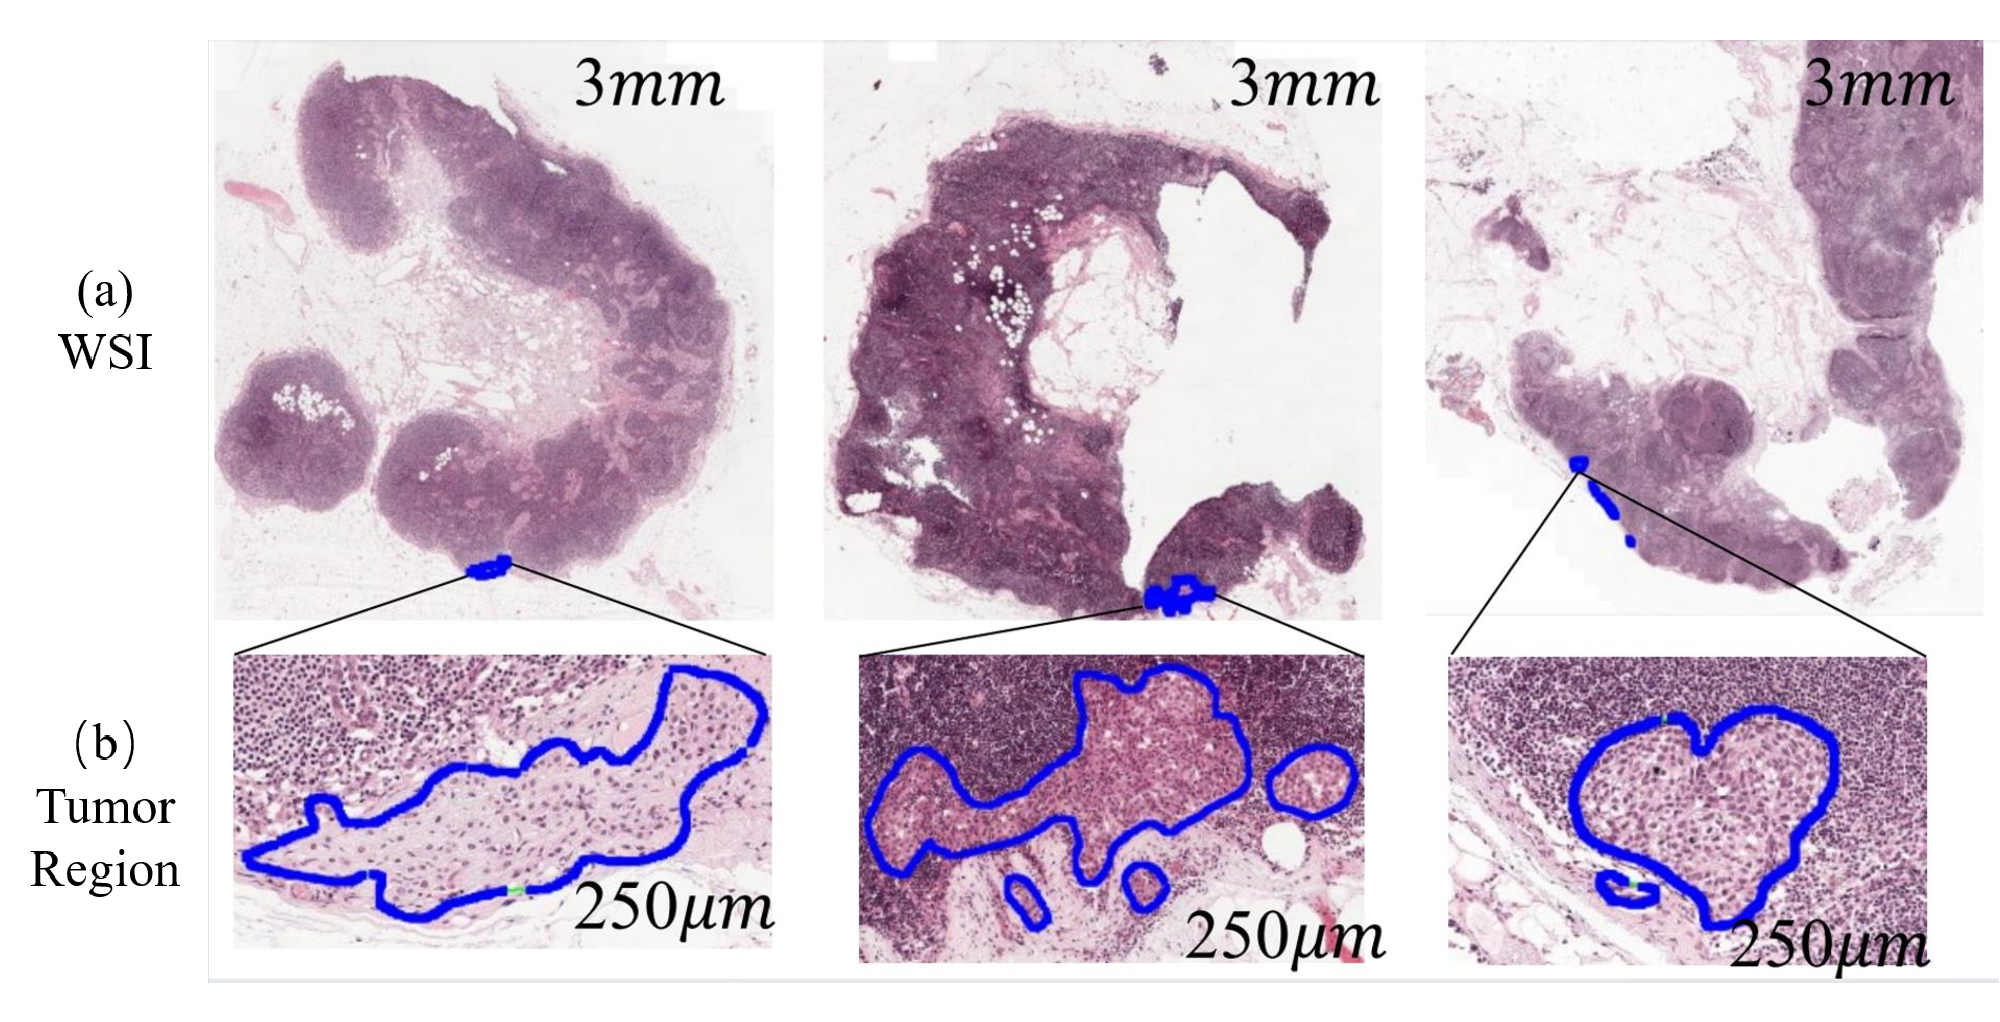
\includegraphics[width=1.0\columnwidth]{figures/fig1.pdf}
    \bicaption[Camelyon16数据集中肿瘤区域相对于正常区域的比例示例图]{Camelyon16数据集中肿瘤区域相对于正常区域的比例示例图}[Example of the proportion of the tumor region to the normal region in the Camelyon16 dataset]{Example of the proportion of the tumor region to the normal region in the Camelyon16 dataset}
    \label{figure1: WSI图像肿瘤区域示意图}
\end{figure}
与此同时,随着人工智能在各领域的蓬勃发展,AI赋能医疗给病理智能诊断提供了可能。国务院印发的《新一代人工智能发展规划》~\cite{NewGenAIDevPlan}着重指出,要加速人工智能在医疗领域的应用,全力推动医疗影像辅助判读等技术的进步。
利用高分辨率数字病理扫描仪通过高效精准的数字化流程,可以将组织切片转换为亿级像素的全幅切片图像(Whole Slide Image, 下文简称病理图像或WSI)~\cite{唐仲平2018全切片图像扫描技术在临床病理诊断工作中的应用},
而这些图像便于存储、传输与共享,打破了时空限制。加之计算机视觉技术的突飞猛进,图像处理、人工智能及机器学习算法持续创新,让病理图像自动化分析从设想走向现实。通过对海量数字病理图像的深度学习,计算机模型有能力捕捉到人类肉眼难以察觉的病变特征,以提高病理诊断的效率与准确性。

然而,针对如此高分辨的WSI图像而言,传统深度学习算法仍有不小挑战:数十亿像素的图片如直接输入到传统的分类器中,将导致难以承担的计算成本;
而若采用采样出的低分辨率的缩略图作为输入,则会不可避免的丢失大量关键信息,造成性能上的损失。
同时,由于病理图像的标注需要大量专家知识,因此细粒度的图像标注过程既耗时又耗力。当前,在仅提供低精度标注的场景下,如何充分挖掘未标注数据的潜力以优化模型效能,已成为数字病理图像分析领域的核心研究方向之一。
\begin{figure}[h]
    \centering
    \captionsetup{font={small, stretch=1.312}}
    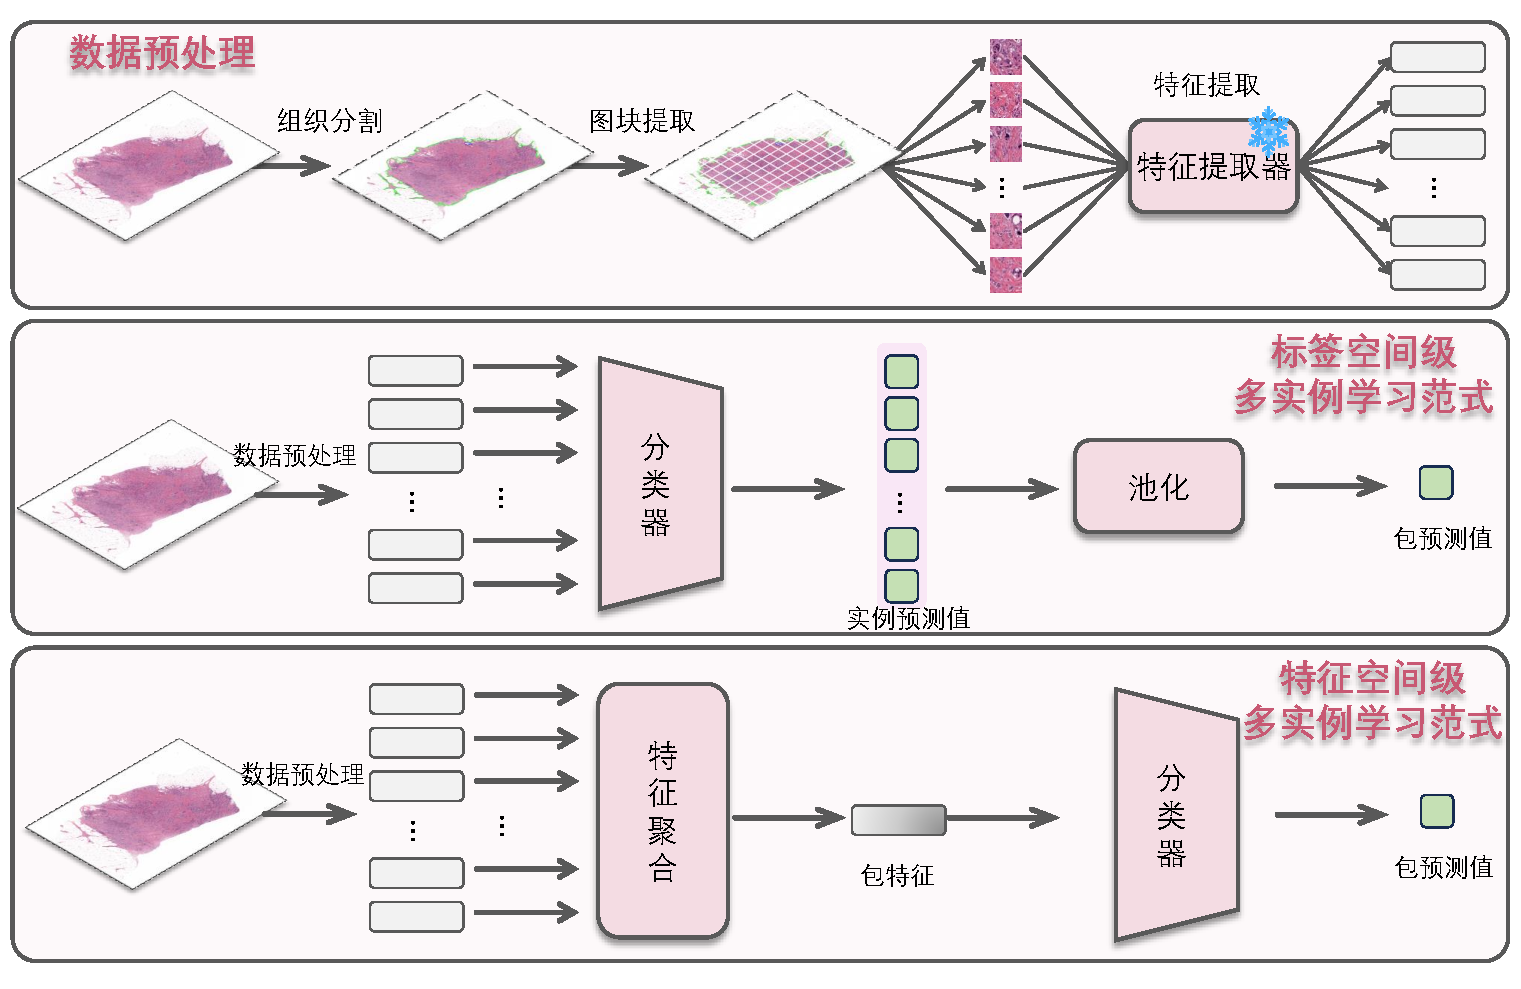
\includegraphics[width=\columnwidth]{figures/多实例学习范式.pdf}
    \bicaption[两种多实例学习范式示意图]{两种多实例学习范式示意图}[The illustration of two paradigms for multiple instance learning.]{The illustration of two paradigms for multiple instance learning}
    \label{figure1: 多实例学习范式}
\end{figure}

多实例学习(Multiple Instance Learning,MIL)\cite{dietterich1997solving,herrera2016multiple}作为一种特殊的弱监督学习框架是业内解决这一类问题的常见技术手段~。
具体而言,每张病理图像都被视为一个“包”(Bag),并会被进一步分割成大量图块(Patch),这些图块被定义为“包”中的“实例”(Instance)。
其目标是在分类标签(如“恶性”或“良性”)作用于整个包的情况下,通过分析实例与包标签之间的关联性,挖掘出关键实例特征,并基于这些信息完成对整张图像的分类。
然而,在病理图像的实际应用场景中,多实例学习框架虽然得到了广泛应用~\cite{li2021dual,lu2021data,shao2021transmil,zhang2022dtfd,tang2024feature},但仍然面临着诸多现实问题。
由于尺寸巨大,切分后的实例数目众多,导致在使用具有较强建模能力的传统ViT~\cite{dosovitskiy2020image}进行实例处理时所需的计算资源消耗巨大,只能采取减少实例数目或更换为线性注意力机制的折中方案。

而近期,一些基于状态空间模型(State Space Model,SSM)~\cite{hamilton1994state}的架构为解决上述问题,提供了新的思路。
Mamba~\cite{gu2023mamba,mamba2}是最近提出的一种具有代表性的基于SSM架构的模型,与ViT相比具有更好的长序列建模能力,而且仅需线性的计算资源。
自从其引入到视觉领域后,在分类~\cite{zhu2024vision,yue2024medmamba,DATE20250218001,yao2024spectralmamba}、检测~\cite{BJHK20241114002,ZGGL202412016,chen2024mim,zhang2025cdmamba}、
分割~\cite{GXXB20250212011,JSGG20240822004,li2025selective,wu2025h}等任务中已经取得了显著的表现,展现出了宏大的应用前景。
然而作为原本被提出解决序列问题的Mamba总是倾向于建模出一种前序Token与后序Token的因果关系,
这与病理图像多实例学习的序列不变特性并不相符~\cite{huang2024localmamba}。并且,其以一维序列作为输入,常常无法完全捕获图像中的二维空间信息。
鉴于此,针对高分辨率数字病理图像分类任务,通过构建基于 Mamba 的模型框架弥合序列相关的 Mamba 模型与序列无关的 WSI 分类任务之间的性能差异,深度挖掘病理图像的空间特征信息,进而优化模型的分类效能,推动数字病理图像计算机辅助诊断准确率的显著提升,具有重要的临床应用价值与学术研究意义。

\section[\hspace{-2pt}国内外研究现状与挑战]{{\heiti\zihao{-3} \hspace{-8pt}国内外研究现状与挑战}}\label{section1: 国内外研究现状与挑战}

\subsection[\hspace{-2pt}数字病理图像分类研究现状]{{\heiti\zihao{4} \hspace{-8pt}数字病理图像分类研究现状}}\label{section1: 数字病理图像分类研究现状}

鉴于数字病理图像分辨率极高,同时细粒度像素级标注较为匮乏,当前研究工作普遍借助多实例学习框架攻克数字病理图像的分类难题。
多实例学习,英文表述为 Multiple Instance Learning,简称为 MIL,部分文献也将其译为多示例学习。
多实例学习的经典范式最早由 Dietterich TG 等学者于 1997 年在药物活性预测研究中首次提出并成功应用~\cite{dietterich1997solving}。
作为弱监督学习领域的典型框架,该技术已受到学术界的广泛关注。其训练数据通常由带有类别标签的包集合构成,每个包内包含多个未标注实例,构成独特的弱监督学习模式。
正包中至少含有一个正实例,负包中只包含负实例。
在多实例学习的训练过程中,只需要提供粗粒度的包级标签(如病人是否患癌),而在实际场景中粗粒度的包级标签往往是易获取的,
从而使得多实例学习非常契合多种实际场景,很多问题可以自然的表述为多实例问题。
以药物活性预测问题为例~\cite{dietterich1997solving},在该问题里,主要的任务目标在于对某一种新分子是否适宜用于制药进行预测。实际情况是,每一个分子都存在着多种可能的低能形状。
所获得的标签信息仅仅是明确了哪些分子是适合制药的,然而对于究竟是分子的哪一种具体低能形状在其是否适合制药这一判定中起到了关键决定性作用,却并不清楚。
鉴于这样的情况,在处理该问题时,便将每一个分子当作是一个 “包”,而分子的每一种低能形状则对应成为这个 “包” 中的一个 “实例”,如此一来,就形成了多实例学习中所定义的实例与包的关系模式。
由于其独有的特性,多实例学习在各个领域都得到了广泛的发展和应用,如目标检测~\cite{hoffman2015detector,wu2015deep,陈钰2016基于,tang2018weakly},语义分割~\cite{xu2019camel},
图像和视频分类~\cite{唐大伟2014壁画图像分类中的分组多实例学习方法,huang2021weakly,wang2013max,chen2006miles,rahmani2006missl,andrews2002support},文本分类~\cite{zhou2009multi},医学图像分类~\cite{ilse2018attention,shao2021transmil,zhang2022dtfd,kanavati2020weakly,li2021dual,chikontwe2020multiple}等。

当前,多实例学习方法主要分为标签空间方法与特征空间方法。标签空间方法基于实例级标签推断聚合策略直接预测包标签,其实例间关系建模能力有限,且在大规模数据集中面临计算效率瓶颈~\cite{campanella2019clinical}。
鉴于此,当前研究重点逐渐转向特征空间方法,这类方法通过整合包内所有实例的特征信息,构建包的嵌入特征表示,进而实现包级标签的预测。
例如,Ilse等人~\cite{ilse2018attention}提出的AB-MIL,在多实例学习框架中引入基于注意力的聚合层,通过神经网络以参数化方式量化每个实例对于包级特征嵌入的贡献。
Li 等学者~\cite{li2021dual}在研究中提出并构建了 DSMIL 方法,通过融合自监督对比学习与金字塔特征融合机制高效提取实例级特征,并创新性地引入非局部注意力模块聚合多尺度实例信息,从而显著提高 WSI 全切片图像分类任务的准确率。
DTFD-MIL~\cite{zhang2022dtfd}引入双层多实例学习框架,将图像分割成多个伪包,通过聚合伪包的预测结果,推断整个病理图像的标签。Zhu等人~\cite{zhu2024dgr}提出DGR-MIL模型,通过引入可学习的全局向量,精准识别最具代表性的实例,并采用交叉注意力机制计算实例间的重要性,有效挖掘病理图像中的关键特征。Shao等人~\cite{shao2021transmil}将Transformer架构引入多实例学习框架中,利用空间位置编码保留空间拓扑结构,并通过注意力机制实现实例间关系的多粒度建模。

Transformer中自注意力机制计算成本高昂,限制了其在大规模图像数据处理任务中的推广与应用。因此,Tang等人~\cite{tang2024feature}通过将病理图像划分为多个区域,显著减少Token数量,并引入线性自注意力机制,降低计算成本的同时有效建模实例间的关系。
然而,这种轻量型的自注意力机制会在一定程度上削弱模型对复杂实例关系的建模能力。
最近提出的Mamba模型~\cite{gu2023mamba}因其高效的计算效率和强大的实例关系建模能力成为了热门模型,
但作为与输入顺序相关的序列模型,Mamba对实例扫描模式非常敏感,这与多实例学习对序列不变性的要求相冲突,
影响了其在病理图像分类任务中的稳定性,限制了其在病理图像分类中的潜力。


\subsection[\hspace{-2pt}视觉Mamba研究现状]{{\heiti\zihao{4} \hspace{-8pt}视觉Mamba研究现状}}\label{section1: 视觉Mamba研究现状}

Mamba最初是在自然语言处理领域提出的,作为一种更有效地处理长序列的架构\cite{gu2023mamba}。
与Transformer \cite{vaswani2017attention}等传统模型不同,Mamba采用了一种选择性状态空间模型(SSM \cite{kalman1960new}),该模型基于内容动态地过滤和处理信息,使模型能够选择性地记住或忽略部分输入。
Mamba在处理速度和可扩展性方面提供了显著的改进,特别是对于较长的序列。
Zhu等人首先将Mamba引入视觉领域研究人员们的视野\cite{zhu2024vision},其在具有强大的建模能力的同时仅需线性计算资源的特点,让其迅速在分类、检测、分割等诸多领域取得令人惊奇的效果。
\begin{figure}[h]
    \centering
    \captionsetup{font={small, stretch=1.312}}
    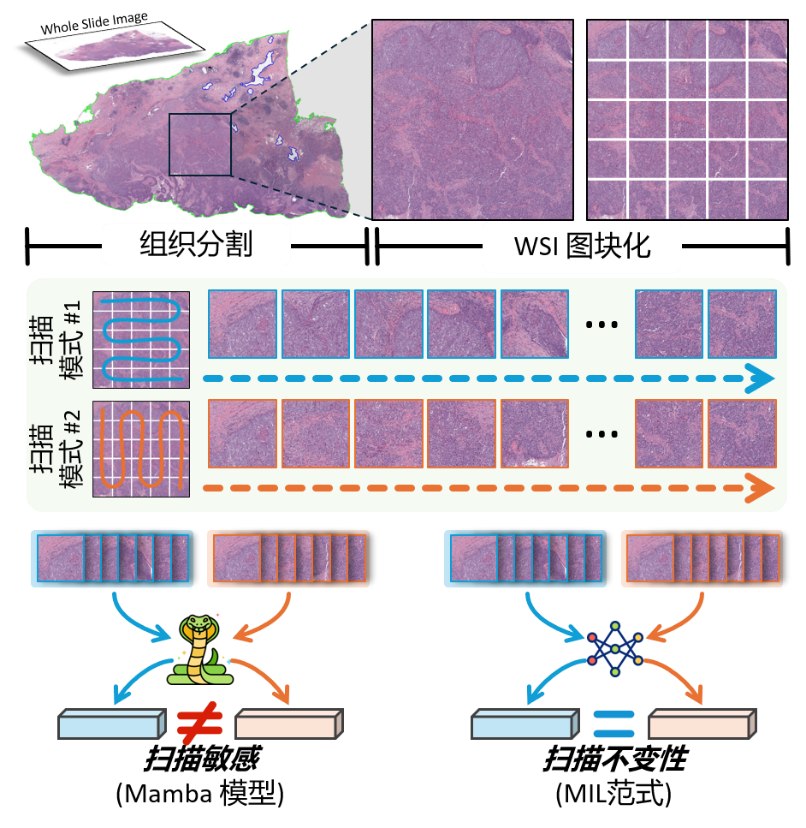
\includegraphics[width=0.7\columnwidth]{figures/Discrepancy1.png}
    \bicaption[Mamba模型与MIL任务差异图]{Mamba模型与MIL任务差异示意图}[Discrepancy between Mamba and MIL for computational pathology tasks]{Discrepancy between Mamba and MIL for computational pathology tasks}
    \label{figure1: Mamba模型与MIL任务差异}
\end{figure}

然而,Mamba作为一种自回归模型,在视觉任务与多实例学习任务中固有地表现出差异,如图\ref{figure1: Mamba模型与MIL任务差异}所示:Mamba假设之前和之后的斑块之间存在因果关系\cite{liu2024vmamba},
而在图像中,不同斑块之间不存在这种因果关系,甚至在多实例学习范式中更是将各个实例视为“平等”实例,并无顺序关联。因此,许多研究通过聚合多种扫描模式来减轻Mamba对序列顺序的敏感性。例如,Vim\cite{zhu2024vision}通过组合来自两个分支(向前和向后)的结果来减轻序列顺序的影响。而Vmamba\cite{liu2024vmamba}采用了四种扫描模式:左上到右下、右下到左上、右上到左下、左下到右上。这些模式综合多个信息序列以提高性能。 LocalMamba~\cite{huang2024localmamba}引入了一种新的局部扫描策略,将图像划分为不同的窗口,综合横向、纵向、局部等多种扫描模式,在保持全局视角的同时有效地捕获局部依赖,大大提高捕获有效图像表示方面的性能。

对于病理图像分类而言,MamMIL\cite{fang2024mammil}结合了Bi-SSM和2D-CAB模块,整合了来自原始、反向和局部序列的扫描模式信息,从而增强了WSI分类。
此外,MambaMIL\cite{yang2024mambamil}将序列重塑成一个矩形,并应用序列重排序操作来垂直扫描新序列,提高了其模拟长序列的能力。
然而,这些方法过度关注输出序列信息的整合,未能从根本上突破序列输入顺序对Mamba建模能力的约束,仅仅是一种妥协的策略,其依旧高度依赖扫描模式和集成形式,使得模型性能不够稳定性。

\section[\hspace{-2pt}本文研究内容与创新点]{{\heiti\zihao{-3} \hspace{-8pt}本文研究内容与创新点}}\label{section1: 本文研究内容与创新点}

本文研究了Mamba架构在病理图像分类中的应用。
虽然Mamba架构在处理病理图像分类任务时,可以解决由于实例数目过多导致的问题,例如计算资源消耗巨大、实例间关系建模不充分等,
但其仍然存在其无法捕获二维空间关系、以及与病理图像多实例学习的序列不变性存在冲突等问题,与病理图像分类任务并不完全适配。
如何缓解甚至消除二者其中的差异依旧是将高效且性能卓越的Mamba架构适配到病理图像领域一个重要的且有挑战性的问题。
因此,本文研究了Mamba架构在病理图像分类中的应用,分别从多扫描模式融合Mamba和扫描不变性Mamba的两个角度开展以下研究:

\textbf{(1)基于多扫描Mamba的高分辨率病理图像分类研究}

针对Mamba一维序列建模所造成图像空间结构捕获能力不足的问题,
本文从Mamba整合多种扫描模式的角度出发,提出基于空间信息增强实现的多扫描Mamba的多实例学习框架(\textbf{M}ulti-scan \textbf{M}amba with \textbf{S}patial information enhancement ,简称M$^2$S-MIL)。
由于常用扫描模式未关注到图像的局部连续性、旋转不变性等特性,该框架采用了多个扫描模式分支作为Mamba的输入,通过设计了区域螺旋扫描和网格扫描等新的扫描模式,
提高Mamba对局部连续性、旋转不变性以及同一序列不同方向的空间关联信息的捕获能力。同时为进一步提升序列的2D空间上下文的感知能力,设计了基于分块局部注意力的2D空间上下文感知模块,
利用区域内的信息整合更进一步提高Mamba对空间能力的捕捉,使Mamba模型更适配于病理图像分类任务。
在3个WSI分析子任务和7个数据集上的大量实验表明,综合多种扫描模式分支,引入空间信息,
能够切实解决Mamba从一维实例序列中空间建模不充分的问题,显著提高模型性能,同时在数字病理图像分类任务中一定程度缓解了使用Mamba模型出现的建模倾向差异难题。​

\textbf{(2)基于扫描不变性Mamba的高分辨率病理图像分类研究}

%利用多扫描模式的信息融合缓解Mamba建模能力与病理图像任务间差异的想法是直截了当的,
%然而这种方法没有本质上突破输入秩序对Mamba建模能力的约束,仅是一种妥协式的策略。
%因此,
本文针对Mamba作为序列相关模型,与病理图像多实例学习的序列不变性存在冲突的问题,从构建扫描不变性Mamba角度出发,提出了基于对比学习策略实现的扫描不变Mamba的多实例学习(\textbf{S}can-invariant \textbf{M}amba with \textbf{C}ontrastive Learning ,简称SMC-MIL)框架。
为了指导 Mamba 学习到不同实例扫描序列中一致的包特征,本文设计了双分支实例序列对比学习框架,通过约束同一Mamba从不同扫描序列获得的包表示及分类结果保持一致,来引导Mamba学习与序列顺序无关的特征。
同时引入基于实例评估的序列对比增强方法,来增加对比学习难度,迫使Mamba在输入序列差异极大的情况下,
学习到对病理图像形成一致表示和决策的能力,成功赋予Mamba良好的序列不变建模和实例识别能力。
实验结果显示,SMC-MIL在继承了Mamba优异计算效率和建模能力的同时,有效降低模型对输入序列顺序的敏感性,
专注于实例无序关系建模,挖掘出更具显著性判别特征的实例,更好地适配病理图像分类任务。

本文提出的M$^2$S-MIL模型与SMC-MIL模型分别从多扫描模式Mamba和扫描不变性Mamba的两个角度出发,对数字病理图像分类任务中Mamba的应用进行深入的剖析和研究。
M$^2$S-MIL模型通过综合多种扫描模式的特征信息,并引入空间上下文感知模块,进一步提升Mamba对2D空间信息的捕获能力,缓解原本一维Mamba模型对2D病理图像空间建模能力不足的问题;
SMC-MIL模型则进一步突破扫描顺序对Mamba建模能力的约束,弥合了原本Mamba的序列敏感性与病理图像多实例学习中序列不变性假设的冲突,
使Mamba架构更加适配病理图像分类任务,并提高了模型挖掘更具判别性区域的能力,从而提升模型性能。

图~\ref{figure1: 主要研究内容}展示了本文的主要研究内容和贡献。

\begin{figure}[h]
    \centering
    \captionsetup{font={small, stretch=1.312}}
    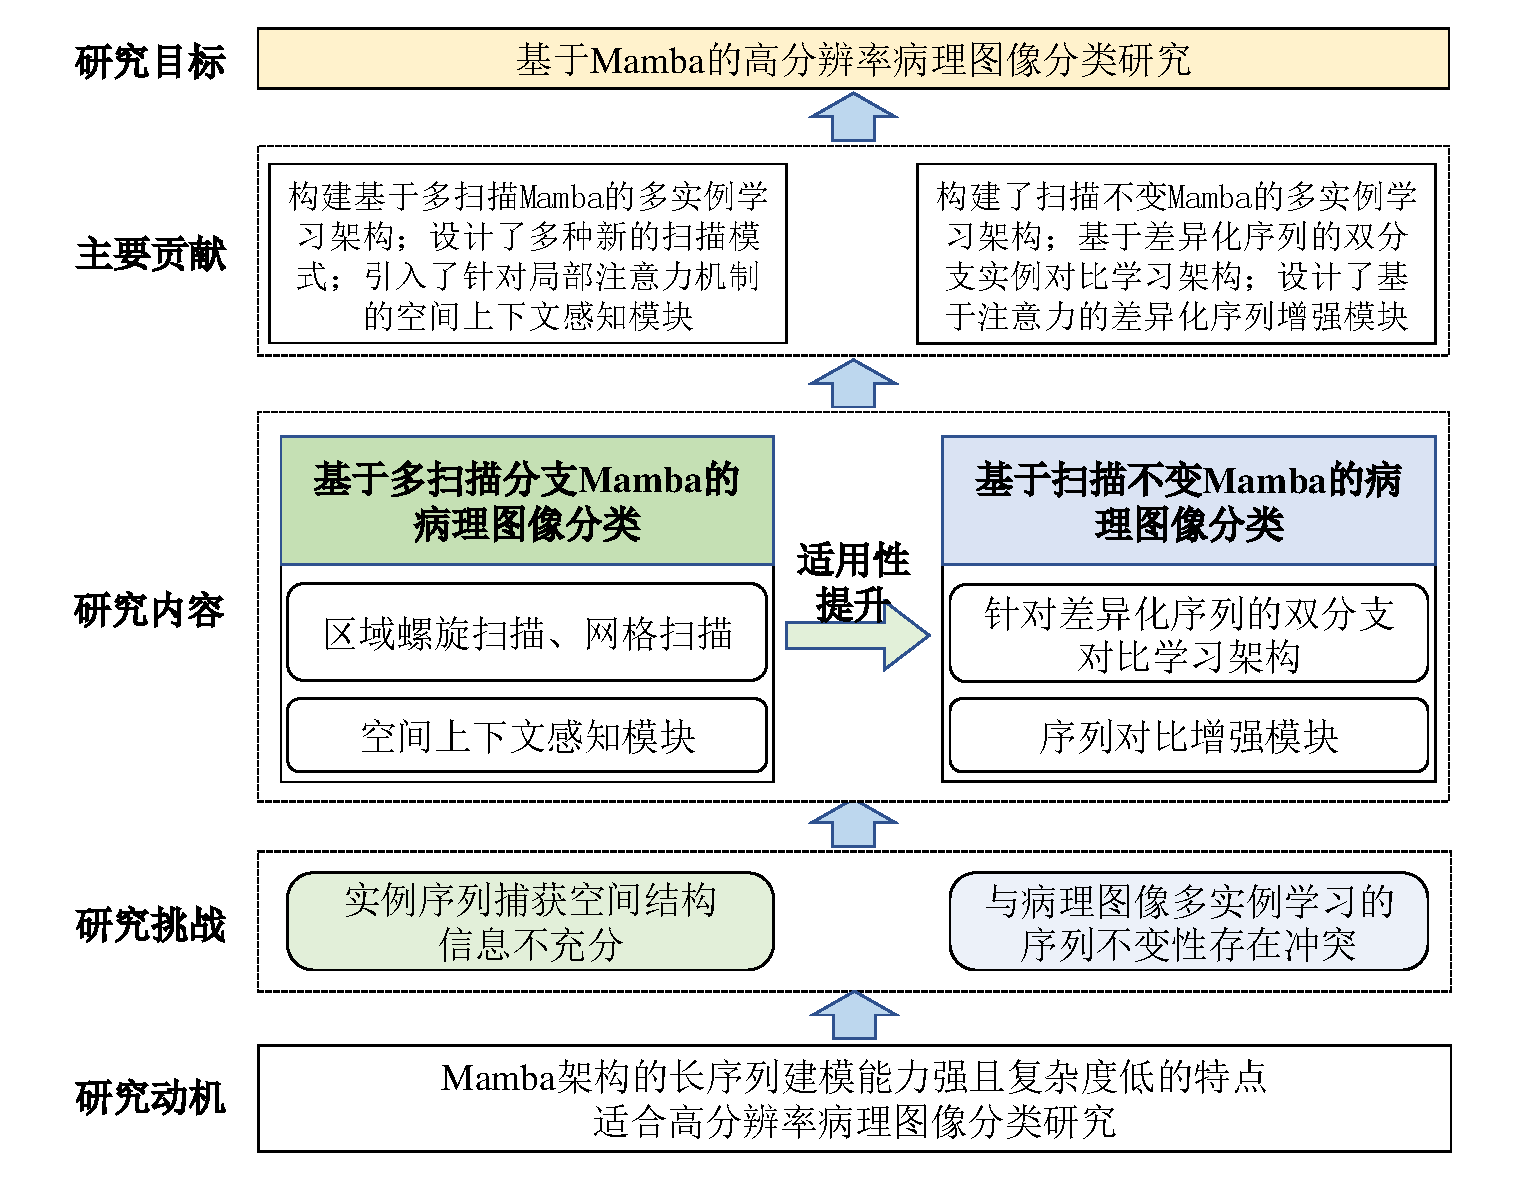
\includegraphics[width=1.0\columnwidth]{figures/研究内容.pdf}
    \bicaption[本文的主要研究内容图]{本文的主要研究内容}[The main research content of this paper]{The main research content of this paper}
    \label{figure1: 主要研究内容}
\end{figure}

\section[\hspace{-2pt}本文组织结构]{{\heiti\zihao{-3} \hspace{-8pt}本文的组织结构}}\label{section1: 本文组织结构}

本文由 5 个章节构成,从多个维度深入探讨基于 Mamba 的高分辨率数字病理图像分类研究。下面为各章节的具体介绍:

第一章:绪论。本章首先阐述高分辨率数字病理图像分类任务的研究背景与科学意义,在系统梳理国内外前沿研究进展的基础上,重点剖析基于视觉 Mamba 架构的数字病理图像分类技术现状及存在的挑战。最后对本文的研究内容和组织结构进行概述。

第二章:相关研究技术与理论。首先系统阐述本课题涉及的基础理论框架,涵盖病理图像多实例学习范式、Mamba 模型架构原理及对比学习机制等核心内容。在此基础上,详细解析所用实验数据集、性能评估指标体系及数字病理图像预处理技术路线。

第三章:基于多扫描融合Mamba的高分辨率医学病理图像分类研究。
首先,通过深入剖析现有 Mamba 病理图像分类算法在空间结构建模能力方面的局限性,提出了基于多扫描Mamba的高分辨率病理图像分类算法(M$^2$S-MIL),最后通过在3个WSI任务和7个数据集上的大量实验证明了M$^2$S-MIL模型的有效性。

第四章:基于扫描不变性Mamba的高分辨率医学病理图像分类研究。首先对基于多扫描序列融合Mamba的病理图像分类算法的不足进行分析介绍,提出了基于扫描不变性Mamba的病理图像分类算法(SMC-MIL),然后介绍了提出的SMC-MIL模型的模型框架以及其中的双分支实例序列对比学习框架和序列对比增强模块,并通过系统的实验验证SMC-MIL模型充分赋予了Mamba扫描不变属性。

第五章:总结与未来展望。总结并分析了本文提出的基于Mamba的高分辨率病理图像分类算法研究的成果及不足,并对未来的研究方向与内容进行了展望。


\chapter[\hspace{0pt}相关研究技术与理论]{{\heiti\zihao{3}\hspace{0pt}相关研究技术与理论}}

\removelofgap
\removelotgap

本章内容共分为六节,\hyperref[section2: 数字病理图像多实例学习]{第一节}详细介绍病理图像分类任务以及主流的多实例学习架构;
\hyperref[section2: Mamba架构]{第二节}介绍Mamba架构;\hyperref[section2: 对比学习]{第三节}介绍第四章方法应用到的对比学习方法及相关理论;
\hyperref[section2: 数据集及评价指标]{第四节}对本文所使用的数据集和评价指标进行介绍;
\hyperref[section2: 病理图像的预处理过程]{第五节}对病理图像的预处理过程进行详细介绍,\hyperref[section2: 本章小结]{第六节}对本章内容进行总结。

\section[\hspace{-2pt}数字病理图像多实例学习]{{\heiti\zihao{-3} \hspace{-8pt}数字病理图像多实例学习}}\label{section2: 数字病理图像多实例学习}

数字病理图像分类属于前沿且极具潜力的交叉研究领域,它将病理学、图像分析和计算机科学等多学科知识进行深度整合。
此领域借助先进算法、机器学习模型和人工智能技术,以实现对WSI图像的全面、精确分析解读,这也是它的核心目标。 
病理图像分类任务通常可分为癌症诊断、亚型分类、生存预测等任务,分别从这些任务角度中辅助病理学家诊断疾病。
数字病理领域,超高分辨率全切片图像(WSI)要完成像素级标注,需投入大量时间与人力。这一难题致使基于像素级标签开展的传统深度学习病理图像分类,难以施展。在此背景下,凭借独特优势,基于多实例学习范式的数字病理图像分类,逐渐成为该领域的常用方法。

多实例学习~\cite{dietterich1997solving}是弱监督学习的重要分支,其核心思想是处理数据标注在“包”(Bag)级别而非单个实例级别的场景。具体而言,每个数据包包含多个实例,但仅包级别标签已知。经典假设为:若一个包中至少存在一个正实例(Positive Instance),则该包被标记为正类;若所有实例均为负类,则包标记为负类。此范式由Dietterich等人在1997年药物分子活性预测研究中首次提出,并逐渐拓展至计算机视觉、自然语言处理及生物医学等领域。

具体来说,对于在病理图像分类任务而言,一张WSI图像$\mathnormal{X}$将作为一个包,将之切分为多个小图块,将每个图块Patch作为一个实例$x_i$,进而得到实例集合$\mathnormal{X} =\{x_i\}^N_{i=1}$。
需注意,不同包所包含的实例数目$N$并不固定。在任何分类任务里,包$\mathnormal{X}$都附带已知的标签信息$\mathnormal{Y}\in \{0,1\}$,而实例标签$y_i$的具体取值$\{0,1\}$处于未知状态。
以二分类任务为例,包的预测标签\(\mathnormal{Y}\)满足公式:
\begin{equation}
    \mathnormal{Y}=\left \{
    \begin{array}{cl}
        0 &  if \space {\sum_{i}^{N}y_i=0} , \\ 
        1 & otherwise.
    \end{array}\right.
    \label{eq2}
\end{equation} 
而多实例学习模型 $\mathcal{M}(\cdot)$ 的目标是利用所有实例预测包的标签 $\hat{\mathnormal{Y}}\leftarrow\mathcal{M}(\mathnormal{X})$。

早期的方法倾向于预测出每个实例的标签后,再以此推断出包标签。这种方法称之为标签空间级的方法。这类方法非常直观,充分利用了多实例学习的定义,但其实例间关系建模能力有限,且在大规模数据集中面临计算效率瓶颈~\cite{campanella2019clinical} 。鉴于此,当前研究重点逐渐转向特征空间方法,这类方法通过整合包内所有实例的特征信息,构建包的嵌入特征表示,进而实现包级标签的预测。大量的研究证明基于特征空间的方法表现出比标签空间级方法更强的性能。

自Ilse等人\cite{ilse2018attention}提出AB-MIL后,基于注意力的特征空间方法已成为业内主流。该方法通过构建基于上下文感知的注意力机制,动态计算每个实例在包特征嵌入空间中的注意力权重,并据此生成最终的包级特征表示。
例如,DTFD-MIL~\cite{zhang2022dtfd}引入双层多实例学习框架,将图像分割成多个伪包,同样使用注意力机制聚合伪包的预测结果,推断整个病理图像的标签。
Zhu等人~\cite{zhu2024dgr}提出DGR-MIL模型,通过引入可学习的全局向量,精准识别最具代表性的实例,并采用交叉注意力机制计算实例间的重要性,有效挖掘病理图像中的关键特征。
Shao等人~\cite{shao2021transmil}将Transformer架构引入多实例学习框架中,利用空间位置编码保留空间拓扑结构,并通过注意力机制实现实例间关系的多粒度建模。
然而Transformer中自注意力机制计算成本高昂,诸多工作只能采取缩减token数量或采用线性的注意力机制等折中方式将这种复杂模型应用于病理图像分类任务中\cite{tang2024feature}。


\section[\hspace{-2pt}Mamba架构]{{\heiti\zihao{-3} \hspace{-8pt}Mamba架构}}\label{section2: Mamba架构}

如图\ref{figure1: Mamba架构示意图},Mamba架构是由Albert Gu和Tri Dao等人于2023年提出的新型序列建模框架~\cite{gu2023mamba},其核心创新在于将状态空间模型(SSM)与选择性机制(Selective Mechanism)相结合,
突破了传统Transformer模型在长序列建模中的局限性。该架构通过建立线性时间复杂度与序列长度的关系,显著提升了模型处理长序列依赖的能力,在自然语言处理、基因组学分析、计算机视觉等领域展现出显著优势。

从数学基础来看,Mamba架构以连续时间状态空间模型为理论框架。其核心微分方程可表述为:
\begin{equation}
\begin{aligned}
    h'(t)&=\mathbf{A}h(t)+\mathbf{B}x(t),\\
    y(t)&=\mathbf{C}h(t) +\mathbf{D}x(t),
\end{aligned}
\label{eq3}
\end{equation}
其中$\mathbf{A}$为状态转移矩阵,$\mathbf{B}$、$\mathbf{C}$分别为输入/输出投影矩阵, $\mathbf{D}$为跳跃连接项。通过零阶保持法(Zero-order Hold)的离散化处理,如公式~\ref{eq4}所示:
\begin{equation}
\begin{aligned}
    \mathbf{\bar{A}}&=\exp(\Delta\mathbf{A}),\\
    \mathbf{\bar{B}}&=(\Delta\mathbf{A})^{-1}(\exp(\Delta\mathbf{A})-\mathbf{I})\cdot\Delta\mathbf{B}.
\end{aligned}
\label{eq4}
\end{equation}
模型将连续系统转化为适用于离散序列的递归计算形式,这一过程在保持系统动态特性的同时实现了计算可行性。
与传统递归神经网络不同,Mamba引入了输入依赖的参数动态化机制,通过函数$\mathbf{B},\mathbf{C},\Delta=f_\theta(x_t)$实现参数矩阵的实时生成,使模型能够根据当前输入特征自适应调整状态转移模式。

\begin{figure}[h]
    \centering
    \captionsetup{font={small, stretch=1.312}}
    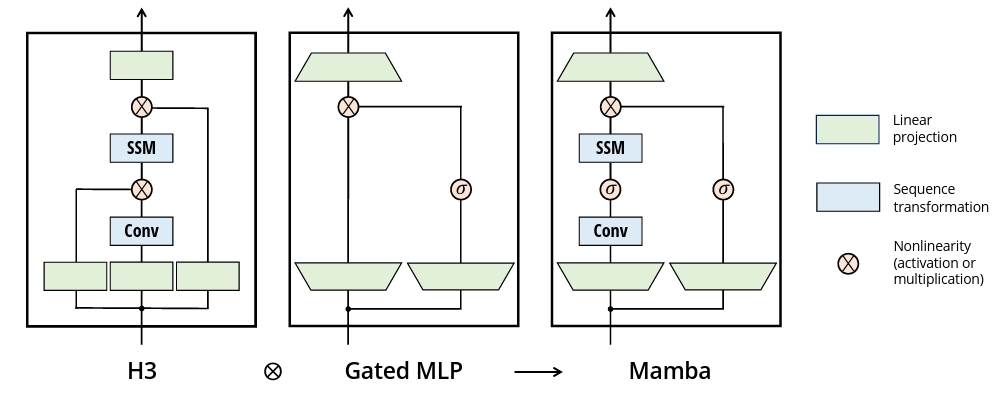
\includegraphics[width=1.0\columnwidth]{figures/RelatedWork/Mamba架构.png}
    \bicaption[Mamba架构示意图]{Mamba架构示意图~\cite{gu2023mamba}}[Illustration of the Mamba architecture]{ Illustration of the Mamba architecture~\cite{gu2023mamba}}
    \label{figure1: Mamba架构示意图}
\end{figure}
在架构设计层面,Mamba通过三个关键创新实现突破:首先,提出选择性扫描算法(Selective Scan Algorithm),通过时间步长参数$\Delta$的动态调节,实现高频信号密集采样与低频信号稀疏处理的智能平衡;其次,开发硬件感知并行化技术,利用GPU内存层级特性优化扫描操作的计算模式,在保持线性时间复杂度的同时实现并行加速;最后,采用模块化堆叠结构,通过交替堆叠SSM块与门控前馈网络构建深度模型,配合残差连接和层归一化技术确保梯度有效传播。实验数据显示,在PG19长文本建模任务中,该架构的困惑度相比Transformer降低23\%,训练速度提升5.2倍~\cite{gu2023mamba}。

相较于传统Transformer的 $O(N^2)$复杂度,Mamba在序列长度为N时实现$O(N)$ 的时间与空间复杂度,这一特性使其在万Token级别的高分辨数字病理图像等场景展现独特优势。
但其本质作为序列敏感型模型,对输入实例的排列顺序具有高度依赖性。
这一特性与多实例学习任务中固有的包级序列不变性要求存在根本性冲突,同时也和视觉任务存在偏差,导致模型在病理图像分类等需弱监督定位的关键场景中易受实例顺序扰动影响,制约模型性能的稳定性与可重复性,并影响其在视觉任务更广泛的应用。


\section[\hspace{-2pt}对比学习]{{\heiti\zihao{-3} \hspace{-8pt}对比学习}}\label{section2: 对比学习}

对比学习作为一种自监督学习范式,通过构建正负样本对的差异性建模实现数据表征学习,已经逐渐成为计算机视觉领域的研究热点之一。其核心在于最大化语义相似样本的嵌入相似度,同时最小化不相关样本的关联性。该方法突破了传统监督学习对人工标注的依赖,其表达式如下所示:
\begin{equation}
\label{equation2: infoNCE}
\mathcal{L} = - \text{log}\frac{\text{exp}(cos(f(x), f(x^+)) / \tau)}{\text{exp}(cos(f(x), f(x^+)) + \sum_{j=1}^{N} \text{exp}(cos(f(x), f(x^-))}.
\end{equation}
图\ref{figure1: 对比学习结构示意图}展示了一些具有代表性的对比学习结构。根据对比学习是否有负样本可以将对比学习分为两类:基于负样本的对比学习、无负样本的对比学习,以下将分别介绍。

\subsection[\hspace{-2pt}基于负样本的对比学习]{{\heiti\zihao{4} \hspace{-8pt}基于负样本的对比学习}}\label{section2: 基于负样本的对比学习}

基于负样本的对比学习方法通过显式地构造负样本对来实现特征判别,代表模型包括SimCLR~\cite{chen2020simple}和MoCo~\cite{he2020momentum}。其核心在于构建动态负样本队列,利用InfoNCE损失函数进行噪声对比估计。
以MoCo v2为例,通过动量编码器(动量系数0.999)维护包含65,536个负样本的特征字典,在ImageNet线性评估协议下达到71.1\%的Top-1准确率~\cite{chen2020improved}。
但该方法面临假负例(False Negative)问题,当负样本中真实正例比例超过5\%时,模型性能下降23\%~\cite{chen2021incremental}

\begin{figure}[h]
    \centering
    \captionsetup{font={small, stretch=1.312}}
    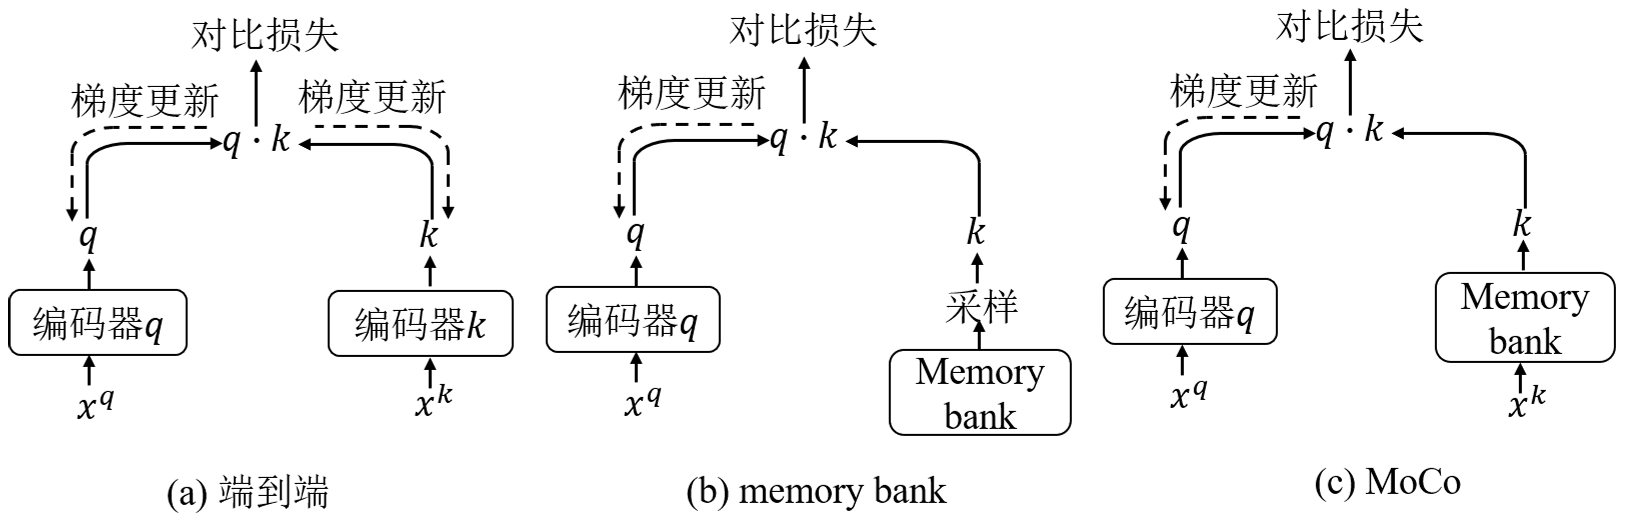
\includegraphics[width=1.0\columnwidth]{figures/RelatedWork/对比学习结构.png}
    \bicaption[对比学习结构示意图]{对比学习结构示意图}[ Contrastive Learning structure diagram]{ Contrastive Learning structure diagram}
    \label{figure1: 对比学习结构示意图}
\end{figure}


%其中,图像$x$经由网络$f(\cdot)$后映射到特征空间,$x^+$,$x^-$分别代表$x$的正样本以及负样本,$N$为负样本数量。$cos(\cdot)$是余弦相似度,$\text{exp}(\cdot)$为以e为底的指数函数。

%Chen等人\cite{SimCLR}提出了一个简单有效的无监督对比学习框架-SimCLR,旨在通过比较不同视角下图像的特征表示来学习强大的特征提取网络。SimCLR的核心思想是利用数据增强来产生正样本对,即从同一张图像中通过随机的数据增强操作(如裁剪、颜色变换等)生成两个视角,然后使来自同一图像的特征相互靠近,同时使得来自不同图像的特征尽可能地远离。尽管SimCLR在无监督特征学习方面取得了显著的成果,但其有一个明显缺点,即SimCLR的效果很大程度上依赖于对比损失函数中大量不同的负样本对,为了达到最佳性能,需要批次大小很大,这对计算资源的要求较高。He等人\cite{MoCo}提出的MoCo算法通过引入一个动态字典来存储样本特征表示解决了此问题。这个字典是一个队列,新的样本特征进入队列时,旧的样本特征被移除,以保持队列的固定大小。MoCo可通过此字典高效地采样大量负样本,因此不再需要使用很大的批次便可达到最佳效果。这些无监督对比学习方法特别适合于数据量大但未标注的场景,能够有效地利用大量未标注数据来学习有意义的特征表示。

% 通过无监督对比学习,模型能够捕捉到数据的内在结构和丰富的特征信息,这为后续的监督学习任务,如分类、检测等,提供了强大的预训练模型。此外,该方法也在自然语言处理、图数据分析等领域展现出了广泛的应用潜力。

\subsection[\hspace{-2pt}无负样本的对比学习]{{\heiti\zihao{4} \hspace{-8pt}无负样本的对比学习}}\label{section2: 无负样本的对比学习}

为解决负样本偏差问题,BYOL~\cite{grill2020bootstrap}等框架摒弃负样本依赖,采用非对称网络架构进行自蒸馏学习。
通过在线编码器(Online Encoder)与目标编码器(Target Encoder)的交互更新,结合预测头(MLP Projector)实现特征一致性约束。
实验表明,在ImageNet数据集上,BYOL使用ResNet-50骨干网络可达到74.3\%的线性分类准确率,且对批处理大小敏感性降低80\%。
但该方法需严格防止模型坍塌(Model Collapse),通常需保留BatchNorm层作为隐式正则化器。



\section[\hspace{-2pt}数据集及评价指标]{{\heiti\zihao{-3} \hspace{-8pt}数据集及评价指标}}\label{section2: 数据集及评价指标}

病理图像分类任务通常可分为癌症诊断、亚型分类、生存预测等任务。
从计算机视觉视角来看,癌症诊断本质上是图像二分类任务;癌症亚型分类,属于图像多分类范畴;而癌症生存预测,对应图像回归预测任务。接下来这一节,将围绕这三项子任务,对相关数据集、模型评估指标等展开介绍 。

\begin{table}[h!]
\small    % 设置表格字体为5号
\setstretch{1.245}        % 设置具有指定弹力的橡皮长度(原行宽的1.2倍)
\captionsetup{font={small, stretch=1.512}}
\centering\bicaption[癌症诊断、分型病理图像数据集详情表]{癌症诊断、分型病理图像数据集详情表。\# 代表具体数目}[Table of Cancer diagnosis, classification WSI dataset details]{Table of ccancer diagnosis, classification WSI dataset details. \# denotes the number of it.}    % 中英文标题
\begin{tabularx}{\textwidth}{lC@{}C @{\hspace{2pt}}C@{\hspace{2pt}}C@{\hspace{2pt}}C}
\toprule
数据集 & \# 病例 & \#WSI & \# 平均图块 & \# 最大图块 & \#最小图块 \\
%\cline{2-5}
%& \raisebox{-2pt}{训练集} & \raisebox{-2pt}{验证集} & \raisebox{-2pt}{测试集} & \raisebox{-2pt}{总数} \\
\midrule
CAMELYON & 370 & 899 & 8108 & 44402 &140 \\
TCGA-NSCLC & 956 & 1053 & 10302 & 43637 &85 \\
TCGA-BRCA & 1062 & 1131 & 8746 & 36618 &283 \\
BRACS     & 189  & 547 & 8429 &  22020 & 106 \\
\bottomrule
\end{tabularx}
%\vspace{-20pt}
\label{table2: dataset1}
\end{table}


\begin{table}[h!]
    \small    % 设置表格字体为5号
    \setstretch{1.245}        % 设置具有指定弹力的橡皮长度(原行宽的1.2倍)
    \captionsetup{font={small, stretch=1.512}}
    \centering\bicaption[生存预测病理图像数据集详情表]{生存预测病理图像数据集详情表。\# 代表具体数目}[Table of Survival prediction Pathology image dataset details]{Table of survival prediction pathology image dataset details. \# denotes the number of it.}    % 中英文标题
    \begin{tabularx}{\textwidth}{lC@{}C @{\hspace{2pt}}C@{\hspace{2pt}}C@{\hspace{2pt}}C}
    \toprule
    数据集 & {\# 病例} & \# WSI & \# 平均图块 & \# 最大图块 & \#最小图块 \\
    %\cline{2-5}
    %& \raisebox{-2pt}{训练集} & \raisebox{-2pt}{验证集} & \raisebox{-2pt}{测试集} & \raisebox{-2pt}{总数} \\
    \midrule
    TCGA-LUAD & 478 & 541 & 10629 & 45783 &85 \\
    TCGA-LUSC & 478 & 512 & 10395 & 33594 &158 \\
    TCGA-BLCA & 376 & 457 & 14364 & 34174 &414 \\
    \bottomrule
    \end{tabularx}
    %\vspace{-20pt}
    \label{table2: dataset2}
    \end{table}



\subsection[\hspace{-2pt}数据集]{{\heiti\zihao{4} \hspace{-8pt}数据集}}\label{section2: 数据集}

\textbf{\textcircled{1}癌症诊断数据集}

\textbf{CAMELYON-16}~\cite{bejnordi2017diagnostic}与\textbf{CAMELYON-17}~\cite{bandi2018detection}作为当前开放获取规模最大的乳腺癌淋巴结转移病理诊断基准数据集,均提供病灶转移状态的二元分类标注(转移/非转移)。
其中,CAMELYON-16数据集的训练集包含由荷兰拉德堡德大学医学中心及乌德勒支大学医学中心联合提供的270张全切片数字病理图像,并配备独立划分的129张官方测试样本。
CAMELYON-17数据集则进一步整合荷兰五所医疗机构的病理资源,共收录1000张经过专业标注的WSI影像。
考虑到CAMELYON-17官方测试集500张样本的标注信息尚未开放,本研究仅采用其已公开的500张训练样本(对应100个临床病例及其影像学诊断结论)。
尽管不少研究,如文献~\cite{li2021dual,shao2021transmil,tang2023multiple,tang2024feature},采用CAMELYON-16~\cite{bejnordi2017diagnostic}数据集,对不同模型在癌症诊断任务中的性能展开评估。
然而,该数据集仅包含 400 张病理图像,图像数量的局限性,削弱了评估结果的有效性。鉴于此,本文参照 CLAM~\cite{lu2021data}的设置,将CAMELYON-16 与 CAMELYON-17 数据集整合,
最终形成包含370个病例、899张有效样本(阴性样本591例,阳性样本308例)的融合数据集(见表\ref{table2: dataset1})。经预处理后,所有病理图像在20倍光学放大倍率下完成分块处理,单张WSI平均生成8108个有效图像块。

\textbf{\textcircled{2}亚型分类数据集}

本文采用了TCGA肺癌数据集、浸润性乳腺癌数据集、和乳腺癌亚型数据集作为亚型分类的评估数据集。其相关数目详情如表\ref{table2: dataset1}所示。

TCGA肺癌数据集(\textbf{TCGA-NSCLC})是由美国国家癌症研究所(National Cancer Institute, NCI)开发的癌症数据共享系统(The Cancer Genome Atlas, 简称TCGA)。
TCGA包括肺鳞状细胞癌(TCGA-LUSC)和肺腺癌(TCGA-LUAD)两类数据,TCGA-LUSC的 478个病例中有512个WSI,
TCGA-LUAD 478个病例中有541个WSI,共1053个WSI。该数据集仅给出了图像级别的标签。和CAMELYON数据集相比,它的阳性样本中肿瘤区域明显大很多。
TCGA 数据集采用了跟 CAMELYON 数据集一样的数据预处理方法。经过处理后,每一幅放大 20 倍的图像大概能产生 10300 个图像块。TCGA 数据集仅仅提供了图像类别的标注信息,并没有提供细致的像素标注内容。

浸润性乳腺癌数据集(Breast Invasive Carcinoma, \textbf{BRCA})是肿瘤基因组图谱大型国际研究项目(TCGA)的一个子项目,致力于了解和研究乳腺癌(BRCA)的基因组特征。BRCA项目系统地收集了来自不同乳腺癌患者队列的肿瘤样本,包括原发肿瘤和转移瘤,以及正常对照组织样本(如非癌乳腺组织)。其中浸润性导管癌(IDC) 779张,浸润性小叶癌(ILC) 198张。

\textbf{BRACS}~\cite{brancati2022bracs}是一个同时用于粗粒度和细粒度分型的乳腺癌亚型数据集。其建立在帕斯卡尔基金会(IRCCS Fondazione Pascale)、美国国家研究委员会(National Research Council CNR)的高性能计算与网络研究所(ICAR)和IBM苏黎世研究中心之间的一项协议之上,该协议旨在“通过组织学图像的自动分析来识别乳腺癌病理学中的非典型肿瘤的方法和工具的开发”。在粗粒度的BRACS分型任务中,每个WSI可分为良性(Benign)、非典型(Atypical)和恶性肿瘤(Malignant)。在细粒度的BRACS分型任务中,将每一种WSI分为正常(Normal)、病理良性(Pathological Benign, PB)、普通型导管增生(Usual Ductal Hyperplasia, UDH)、不典型导管增生(Atypical Ductal Hyperplasia, ADH)、扁平上皮不典型(Flat Epithelial Atypia, FEA)、导管原位癌(Ductal Carcinoma in Situ, DCIS)和浸润性癌(Invasive Carcinoma, IC)。其中Normal、PB、UDH被分为良性病灶;FEA、ADH被归类为非典型(Atypical);DCIS和IC被归为恶性肿瘤(Malignant)。BRCAS数据集被官方划分为395个WSIs的训练集、65个WSIs的验证集和87个WSIs的测试集以用于评估。

\textbf{\textcircled{3}生存预测数据集}

癌症预后生存分析的核心,是量化评估患者群体时序生存概率的分布特征,具体涵盖术后存活期预测、复发风险分层及生存状态演化建模等临床关键维度。
本研究选取TCGA数据库中肺腺癌(\textbf{TCGA-LUAD})、肺鳞癌(\textbf{TCGA-LUSC})及膀胱尿路上皮癌(\textbf{TCGA-BLCA})三个项目的临床随访数据构建愈后预测模型。
需要特别说明的是,与上文所述诊断及分型任务不同,生存预测模型以独立病例为最小分析单元:
TCGA-LUAD与TCGA-LUSC项目沿用分型研究中的原始影像数据,但重新构建了包含生存时间、复发状态等临床终点的标注体系;
TCGA-BLCA数据集则专门收录376例膀胱尿路上皮癌(Bladder Urothelial Carcinom)患者的完整临床随访记录。
三个数据集的相关数目详情见表\ref{table2: dataset2}。
在实验设计层面,通过整合多中心临床数据构建生存分析框架,重点考察模型对患者个体化生存曲线的预测效能。

\subsection[\hspace{-2pt}评价指标]{{\heiti\zihao{4} \hspace{-8pt}评价指标}}\label{section2: 评价指标}

在癌症诊断与分型分类模型的性能评估中,本研究仿照相关文献~\cite{tang2024feature,tang2023multiple},采用标准化的评价指标体系。
基于分类任务的特征差异,分别选用准确率、ROC曲线下面积(AUC)及F1分数作为核心评估参数:
针对具有二分类特性的肿瘤诊断问题,采用二元F1分数(F1-binary)进行量化分析;而对于涉及多类别判别的癌症亚型分类任务,则选用宏观F1分数(F1-macro)作为评价基准。
AUC 对类别分布不均衡具有较强鲁棒性,且对分类决策阈值变化具有较低敏感性,能够有效量化模型的分类效能。鉴于上述优势,本研究将 AUC 作为核心评价指标,并在消融实验环节着重分析模型的AUC 表现。

在生存预测任务中,本研究依据文献~\cite{yao2020whole,chen2021multimodal,zhou2023cross,wulczyn2020deep,zhu2017wsisa}的设置,选取一致性指数(Concordance Index, C-index)~\cite{harrell1996multivariable}作为生存分析模型的核心评估指标。
该指标在继承AUC评估特性的基础上,针对生存数据特有的删失(censored data)问题进行了算法扩展,可系统评估模型的判别效能——即通过个体风险评分对生存时间进行可靠排序的能力。其数学表达式如\ref{equation3}所示:
\begin{equation}
    \text{C-index} = \frac{
        \sum_{i \neq j} \delta_j \cdot I(T_i < T_j) \cdot I(\hat{S}_i > \hat{S}_j)
    }{
        \sum_{i \neq j} \delta_j \cdot I(T_i < T_j)
    },
    \label{equation3}
    \end{equation}
其中$T_j$表示样本$j$的实际生存时间,$\hat{S}_j$为模型预测的生存概率,${\delta}_j\in \{0,1\}$ 为事件状态指示器($\delta=1$表示发生终点事件)。指示函数$I(\cdot)$在条件成立时取1,否则为0。该计算架构通过约束条件${\delta}_j=1$,确保仅纳入实际发生事件的样本对进行统计评估,从而提升结果的可信度。指标取值范围具有明确临床解释性:当 $\text{C-index}=1$时表征模型具备完全预测能力,而$ \text{C-index}=0.5$则等效于随机猜测。相较于传统AUC指标,C-index的优势在于能够有效处理生存分析中普遍存在的删失数据问题,其评估机制更符合临床研究数据的实际分布特征。

\section[\hspace{-2pt}病理图像的预处理过程]{{\heiti\zihao{4} \hspace{-8pt}病理图像的预处理过程}}\label{section2: 病理图像的预处理过程}

本研究针对数字病理图像高分辨率特性(1-10亿像素)带来的计算挑战,采用多阶段预处理框架实现高效特征提取(图~\ref{figure1: 数字病理图像的预处理过程示意图})。

\textbf{分割组织。}首先基于Openslide库读取WSI数据,通过多尺度分割策略提取有效组织区域。具体操作是先在 32 倍降采样层级下,将图像转换到 HSV 色彩空间,使用中值滤波对图像边缘进行平滑处理,之后依据饱和度通道阈值生成初始二值掩码;
随后实施形态学闭运算消除微米级孔洞,并通过面积阈值过滤非组织区域~\cite{lu2021data}。
为提升算法鲁棒性,系统自动生成包含分割参数及处理日志的元数据文件,支持人工复核与参数微调。

\textbf{划分图块并提取特征。}在20倍光学放大倍率下,采用滑动窗口法从有效组织区域裁剪256×256像素图像块,存储为标准化hdf5格式并记录空间坐标信息。
该尺度选择平衡了细胞形态学特征保留与计算效率,单个WSI可产生10³-10⁴量级图像块(视组织面积而定)。
在特征提取环节,本研究采用了两种特征提取器:其一,采用在 ImageNet 数据集上进行预训练的 ResNet-50 模型~\cite{he2016deep},该模型截断至第三残差块,随后应用自适应均值池化操作,把图像块编码成维度为 1024 的向量;
其二, 在“Mass-100K”上预训练的通用的、用于病理学的自监督视觉编码器UNI~\cite{chen2024towards},同样输出1024维向量。
将提取的特征作为在线深度学习模型监督学习的输入,能大幅缩短训练时间、降低计算成本。基于此构建的特征矩阵,让单个 GPU 在数小时内,就能完成万级全切片图像(WSI)的模型训练。

\begin{figure}[h]
    \centering
    \captionsetup{font={small, stretch=1.312}}
    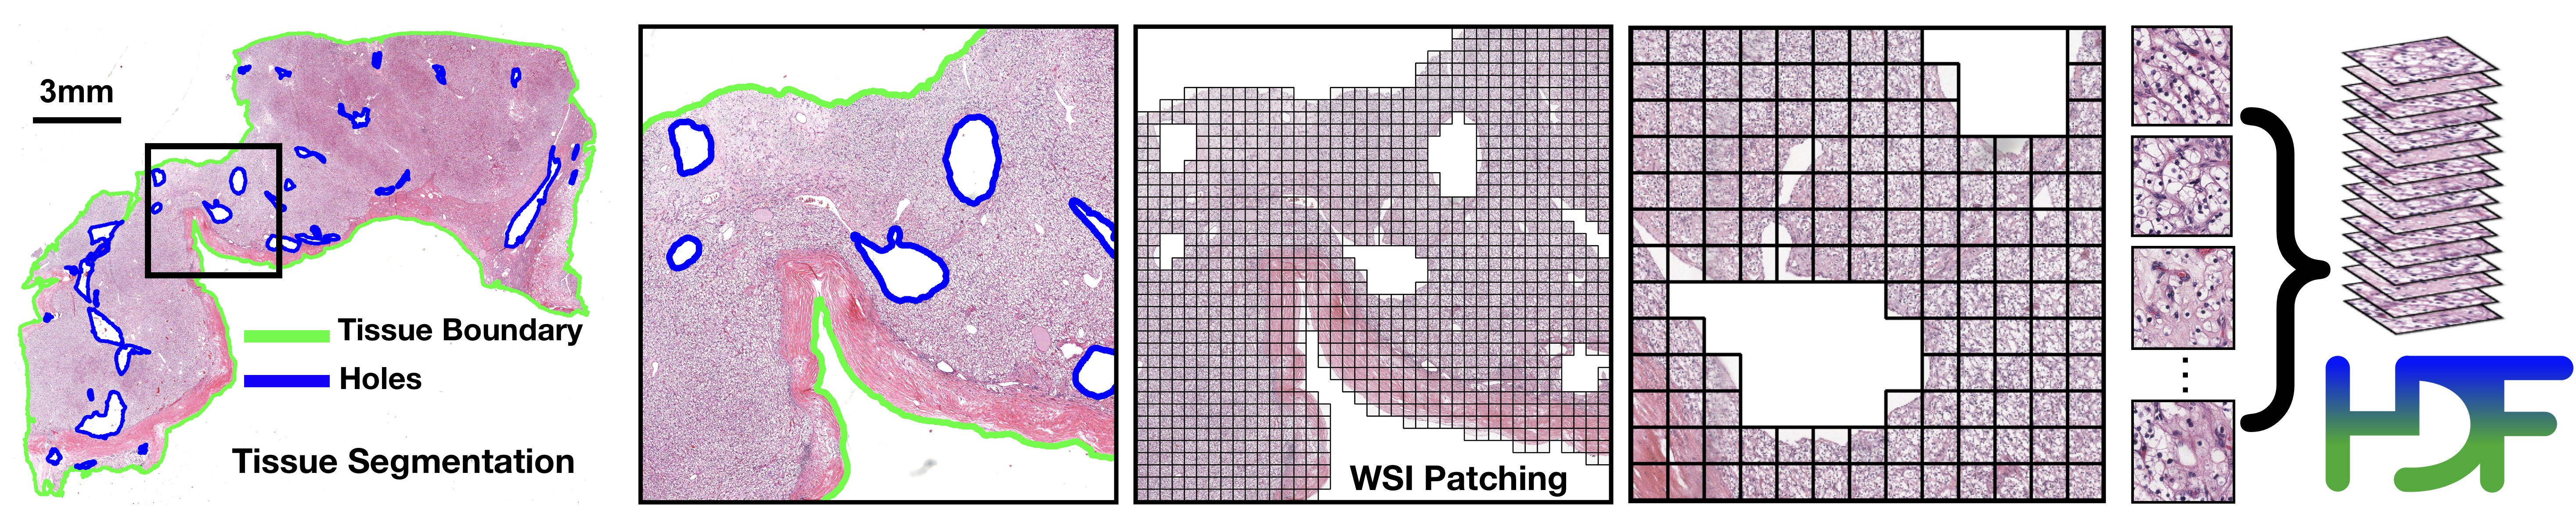
\includegraphics[width=1.0\columnwidth]{figures/RelatedWork/CLAM1.jpg}
    \bicaption[数字病理图像的预处理过程示意图]{数字病理图像的预处理过程示意图~\cite{lu2021data}}[ Illustration of the WSI preprocessing process]{ Illustration of the WSI preprocessing process~\cite{lu2021data}}
    \label{figure1: 数字病理图像的预处理过程示意图}
\end{figure}
\section[\hspace{-2pt}本章小结]{{\heiti\zihao{-3} \hspace{-8pt}本章小结}}\label{section2: 本章小结}

本章首先详细介绍病理图像分类常用的多实例学习范式的分类及发展过程,其次介绍了Mamba架构的特点、优势及迁移至视觉领域所面临的挑战。
然后对后续研究工作所涉及的对比学习等相关技术进行了详细介绍,根据是否使用负样本将其分为基于负样本对比学习和无负样本的对比学习进行了详细阐述。
接着,介绍了本文方法所涉及的数字病理图像分类子任务、数据集和评价指标等,最后介绍了病理图像的预处理阶段。

\chapter[\hspace{0pt}基于多扫描Mamba的高分辨率病理图像分类研究]{{\heiti\zihao{3}\hspace{0pt}基于多扫描Mamba的高分辨率病理图像分类研究}}\label{chapter3: 基于多扫描Mamba的高分辨率病理图像分类研究}
\removelofgap
\removelotgap
本章研究了基于多扫描Mamba的高分辨率病理图像分类研究,通过整合多种扫描模式分支的特征信息,引入病理图像的空间信息,提高Mamba建模2D空间关系的能力,进而提高高分辨率病理图像分类性能。
本章内容共分为四节,\hyperref[section3: 研究动机]{第一节}介绍研究的动机;\hyperref[section3: 问题描述和符号定义]{第二节}介绍问题的描述与符号定义;
\hyperref[section3: 基于空间信息增强的多扫描Mamba模型]{第三节}介绍本章提出的基于空间信息增强的多扫描Mamba模型;
\hyperref[section3: 实验设置及结果分析]{第四节}给出实验设置和结果分析;\hyperref[section3: 本章小结]{第五节}对本章进行总结与讨论。

\section[\hspace{-2pt}研究动机]{{\heiti\zihao{-3} \hspace{-8pt}研究动机}}\label{section3: 研究动机}

%\subsection[\hspace{-2pt}研究动机]{{\heiti\zihao{4} \hspace{-8pt}研究动机}}\label{section3: 研究动机}

病理图像的多实例学习范式中,由于病理图像的分辨率过高,往往面临实例数量庞大、信息繁杂等问题,因此如何高效地提取实例关系并突出关键实例特征一直是多实例学习的核心。
近年来,Mamba模型凭借其高效的计算速度和强大的数据建模能力,逐渐被引入病理图像多实例学习领域,并在特征聚合方面取得了瞩目的效果。
然而,Mamba模型本质是一类序列学习方法,其输入是单个序列,而单个序列无法体现出视觉的空间关系,
因而单个序列扫描模式的Mamba模型的性能会受其空间关系建模的限制。

为了缓解上述所提到的问题,业内主流的解决方案是将多个扫描模式序列的信息进行整合。
然而,如~\ref{figure3: 扫描示意图}左图所示,大多数方法虽然通过类似横向和竖向的扫描模式缓解了Mamba序列敏感特性和视觉任务的差异,但是依旧只是在一维序列中进行,并没有充分利用视觉任务的特性如局部连续性、旋转不变性等,
更没有关注到空间信息的捕获。为此,本章从引入局部连续性、旋转不变性的视觉特性出发,提供了两种新的扫描模式,综合多个扫描模式分支以建模出更全面特征。
此外,本章还通过进一步综合局部空间信息,来提高模型对视觉任务的适配。

\begin{figure}[h]
  \centering
  \captionsetup{font={small, stretch=1.312}}
  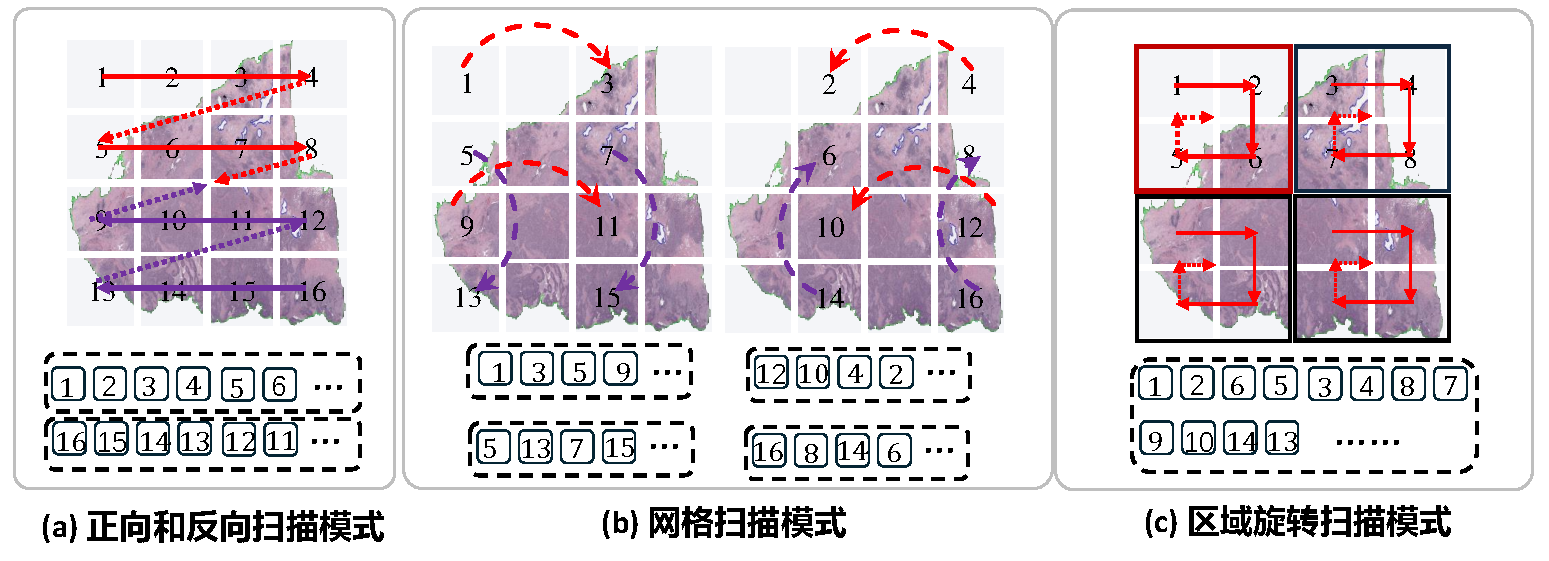
\includegraphics[width=\columnwidth]{figures/多扫描模式.pdf}
  % \captionsetup{justification=justified,singlelinecheck=false}
  \bicaption[常规扫描、网格扫描和区域螺旋扫描示意图]{常规扫描、网格扫描和区域螺旋扫描示意图。}[Schematic diagram of conventional scan, grid scan and region spiral scan]{Schematic diagram of conventional scan, grid scan and region spiral scan.}
  \vspace{-10pt}
  \label{figure3: 扫描示意图}
  \end{figure}

\section[\hspace{-2pt}问题描述和符号定义]{{\heiti\zihao{-3} \hspace{-8pt}问题描述和符号定义}}\label{section3: 问题描述和符号定义}

本研究采用多实例学习范式构建高分辨率病理图像分类模型,其数据集由 WSI 全切片图像与对应标签构成的样本对$(X,Y)$组成,
\begin{equation}
  D=\{(X_1,Y_1),...,(X_j,Y_j),...,(X_n,Y_n)\},
\end{equation}
其中,$n$为数据集样本数量。
每一个WSI切片 $X_j$都被视为一个包,将其Patch视为该包中的实例,可以表示为 $X_j=\{x_i^j\}_{i=1}^N$。实例数量$N$因包而异。
包的类别由其中实例类别综合可得。如果一个包包含至少一个阳性实例,则认为它是阳性的;否则,它被归类为负包:

\begin{equation}
  Y(X)=\left \{
  \begin{array}{cl}
      0 &  if  \sum_{x \in X} y(x) = 0, \\
      1 & otherwise.
  \end{array}\right.
  \label{eq}
\end{equation}

在多实例学习范式中,样本包级标签$Y(X)$作为监督信号已知,而实例级标签$y(x)$则保持隐式状态。
该学习机制的核心目标在于通过聚合实例层特征信息,即用所有实例$\hat{Y}\gets\mathcal{M}\left(X\right)$预测包标签,最终实现病理图像的准确分类。
根据最近流行的方法,MIL预测过程可以分为三个步骤:实例特征提取、实例特征聚合和包分类。具体来说,这个过程可以定义如下:
\begin{equation}
  \hat{\mathnormal{Y}} \leftarrow \mathcal{M}(X):=\mathcal{C}(\mathcal{A}(\mathcal{F}(X))),
\label{eq1}
\end{equation}
其中$\mathcal{F}\left(\cdot\right)$、$\mathcal{A}\left(\cdot\right)$和$\mathcal{C}\left(\cdot\right)$分别是上述步骤的映射函数。

由于同一包中存在大量实例,因此WSI分类问题可以看作是一个长序列建模问题。基于现代状态空间模型(SSM),前人设计了结构化状态空间序列模型(S4)和Mamba等几种适合长序列建模的方法。经典的S4模型可以写成线性递归式:
\begin{equation}
  \begin{aligned}
    h_t&=\mathbf{\bar{A}}h_{t-1}+\mathbf{\bar{B}}x_{t},\\
    y_t&=\mathbf{C}h_t.
  \end{aligned}
  \label{eq32}
  \end{equation}
其中$\mathbf{\bar{A}}$表示离散化后的状态矩阵,$\mathbf{B}$和$\mathbf{C}$表示投影参数,$\mathbf{\bar{B}}$为离散化后的$\mathbf{B}$。另外,模型可以使用卷积模式计算输出:
\begin{equation}
  \begin{aligned}
      \bar{\mathbf{K}}&=(\mathbf{C\bar{B},C\bar{A}\bar{B}},\dots,\mathbf{C}\bar{\mathbf{A}}^{N-1}\bar{\mathbf{B}}),\\
      Y&=X*\bar{\mathbf{K}},
  \end{aligned}
  \label{eq33}
  \end{equation}
其中$K\in R^L$表示一个结构化卷积核,$N$表示输入序列$X$的长度。

Mamba进一步将选择机制集成到S4模型中,通过高效的硬件感知并行算法,使参数动态依赖于输入。
这允许Mamba根据当前上下文有选择地沿着序列传播或忘记信息,从而实现高效的长序列建模。
因此,结合Mamba的多实例学习范式可以被定义:
\begin{equation}
  \hat{Y} \leftarrow \mathcal{M}\left(X\right):=\mathcal{C}(\mathcal{A}(\Psi(\mathcal{F}(X)))),
\end{equation}
其中$\Psi\left(\cdot\right)$表示为Mamba模型。


\section[\hspace{-2pt}基于空间信息增强的多扫描Mamba模型]{{\heiti\zihao{-3} \hspace{-8pt}基于空间信息增强的多扫描Mamba模型}}\label{section3: 基于空间信息增强的多扫描Mamba模型}

\subsection[\hspace{-2pt}方法概述]{{\heiti\zihao{4} \hspace{-8pt}方法概述}}\label{section3: 方法概述}

\begin{figure}[h]
  \centering
  \captionsetup{font={small, stretch=1.312}}
  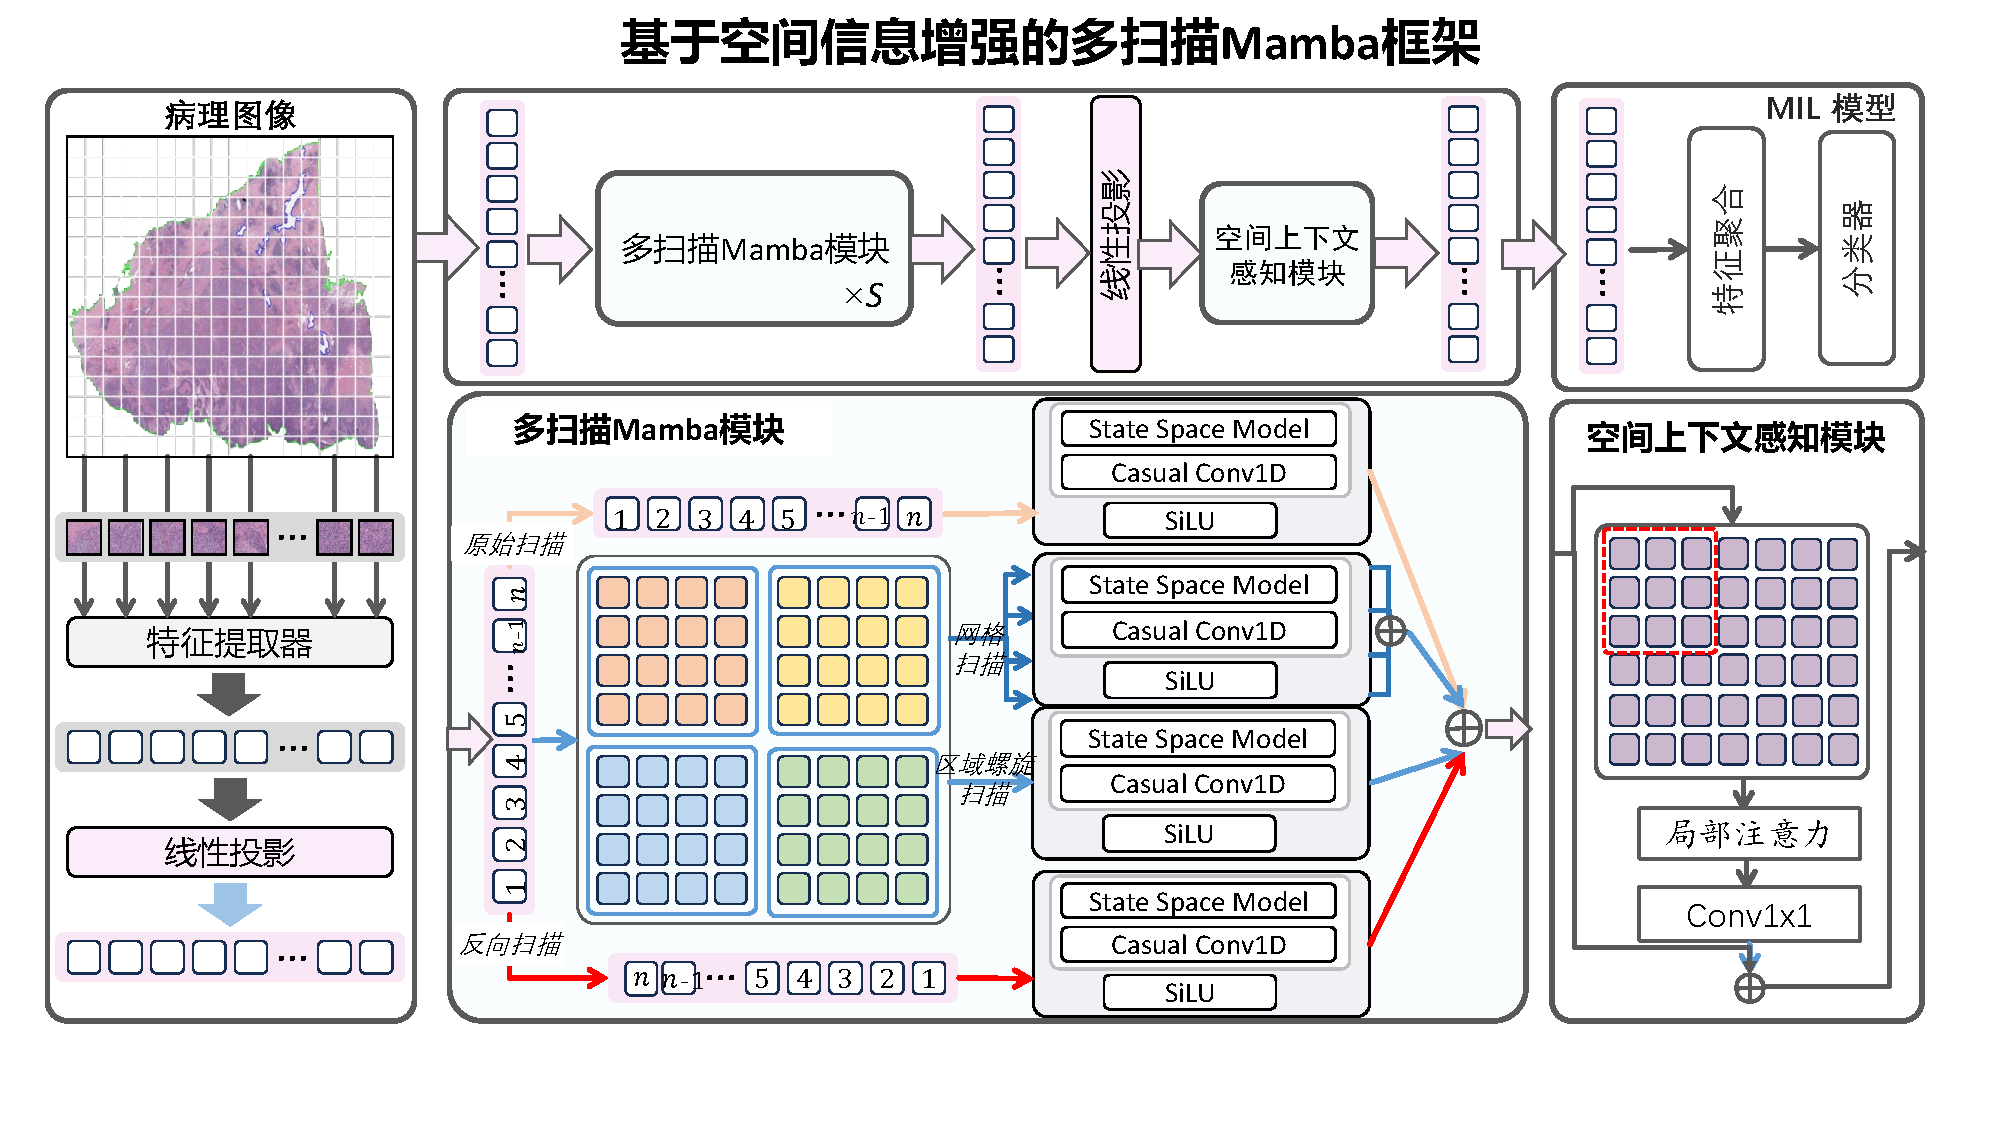
\includegraphics[width=\columnwidth]{figures/MMSMIL.pdf}
  % \captionsetup{justification=justified,singlelinecheck=false}
  \bicaption[基于多扫描Mamba的多实例学习架构示意图]{基于多扫描Mamba的多实例学习架构示意图。}[Illustration of the multi-instance learning architecture with multi-scan Mamba]{Illustration of the multi-instance learning architecture with multi-scan Mamba}
  \vspace{-10pt}
  \label{figure3: 多扫描Mamba}
  \end{figure}

为了解决~\ref{section3: 研究动机}小节中的问题,如图~\ref{figure3: 多扫描Mamba}所示,本章提出了一种名为基于空间信息增强的多扫描Mamba模型,该模型既发挥了Mamba长序列建模能力强的特点,同时也缓解其和视觉2D图像任务间的差异。
具体而言,本研究通过添加区域螺旋扫描和网格扫描等多种扫描模式分支,引入局部连续性、旋转不变性等的2D图像特性。
此外,为了进一步整合2D空间关系信息,本章引入一个2D空间上下文感知模块。总的来说,本研究的贡献如下:
\begin{itemize}
 \item 本研究提出了一种基于多扫描Mamba的多实例学习架构,命名为M$^2$S-MIL。M$^2$S-MIL通过添加区域螺旋扫描和网格扫描等扫描模式,引入2D图像的局部依赖和旋转不变性等,使之更适合病理图像分类任务。
 \item	针对视觉领域的2D属性,设计了新的扫描模式:区域螺旋扫描模式和网格扫描模式,引入了更多局部依赖、旋转不变性等2D空间信息,缓解顺序敏感的Mamba与病理图像分类任务间的差异。
 \item	为了进一步整合提升2D空间关系信息,本章设计了一个2D空间上下文感知模块,采用分块局部注意力,进一步融合局部相邻的实例信息,进一步提高模型性能。
\end{itemize}

\subsection[\hspace{-2pt}预处理与特征提取]{{\heiti\zihao{4} \hspace{-8pt}预处理与特征提取}}\label{section3: 预处理与特征提取}

给定一个WSI图片,参照CLAM~\cite{lu2021data}的设置,本章将之裁剪成一系列$256\times256$的非重叠图块,放大倍数为$20$倍,同时丢弃背景区域(饱和度$< 15$)。
本章采用ResNet-50~\cite{ROYERCARFAGNI2001253}或UNI~\cite{chen2024towards}作为底层特征提取器$\mathcal{F}\left(\cdot\right)$,对每个实例提取特征得到1024维的原始特征。
为了减少特征冗余和计算消耗,使用多层感知器(MLP)层将这些特征从1024减少到512。
数字病理图像的特征提取过程为:
\begin{equation}
  z_i= \mathcal{F}_\varphi(x_i) \in \mathbb{R} ^d.
\end{equation}
在该模型架构中,$\mathcal{F}_\varphi(\cdot)$被定义为骨干特征提取网络,其参数 $\varphi$表示特征学习模块的可训练参数集,通常其不与后续网络一起端到端训练,$d= 512$。
最后,一个WSI由一个连续长序列表示。
本章将之定义为原始扫描序列$Z_{origin}=\{z_i\}_{i=1}^N$,其中$z_i$是$X$的第$i$个实例的提取特征,$N$是实例的个数。

\subsection[\hspace{-2pt}多扫描Mamba模块]{{\heiti\zihao{4} \hspace{-8pt}多扫描Mamba模块}}\label{section3: 多扫描Mamba模块}

为了使Mamba能充分学习到实例间的相互依赖,并缓解其本身因果建模倾向所带来的负面影响,
本章方法提出使用多种扫描模式,以消除单一扫描序列所建模出的偏执,捕获实例间更全面的特征信息。
如图~\ref{figure3: 多扫描Mamba}所示,在多扫描Mamba模块中可分为四个扫描分支:原始扫描序列分支、反向扫描序列分支、区域螺旋扫描分支和网格扫描分支。
首先,原始扫描模式序列被输入Mamba模型以提供常规特征:
\begin{equation}
  Z'_{origin}=\Psi_{origin} (Z_{origin}),
\end{equation}
其中,$\Psi_{origin}(\cdot)$同~\ref{section3: 问题描述和符号定义}小节所示为Mamba模型。 反向扫描序列以初步缓解Mamba不过分学习到正向序列的特有顺序偏执:
\begin{equation}
  Z'_{flip}=\Psi_{flip} (Z_{flip})=\Psi_{flip} (\{z_i\}_{i=N}^1).
\end{equation}
为进一步引入空间信息,本章精心设计了两种新的扫描模式:区域螺旋扫描和网格扫描模式。
其中,区域螺旋扫描被设计以引入局部连续性和旋转不变性等2D图像属性,网格扫描模式用于在一个序列中捕获多个方向上的信息。




具体而言,输入的实例特征序列首先被重塑为2D特征图,初始的二维特征图形式为$H\in \mathbb{R} ^{N\times D}$,
之后转变为$ H \in \mathbb{R} ^{\lceil\sqrt{N}\rceil \times \lceil\sqrt{N}\rceil \times D}$。
重塑后便可如图~\ref{figure3: 扫描示意图}所示的网格扫描方式。网格子序列1可表示为:
\begin{equation}
  %Z_{grid1}=\{z_{ij},i=2k+1,k<=\lfloor \lceil\sqrt{N}\rceil/2\rfloor , k \in \mathbb{N}_0;j=2m+1,m<=\lfloor \lceil\sqrt{N}\rceil/2\rfloor,m \in \mathbb{N}_0.\}
  Z_{\text{grid1}} = \left\{ z_{ij} \,\big|\, 
i = 2k + 1,\, j = 2m + 1,\, 
k, m \in \mathbb{N}_0,\, 
k, m \leq \left\lfloor \frac{\lceil \sqrt{N} \rceil}{2} \right\rfloor 
\right\}.
\label{Z_grid1}
\end{equation}

同理,网格序列集合2、3、4可分别表示为:
\begin{equation}
  \begin{aligned}
  Z_{\text{grid2}} &= \left\{ z_{ij} \,\big|\, 
  i = 2k,\, j = 2m + 1,\, 
  k, m \in \mathbb{N}_0,\, 
  k, m \leq \left\lfloor \frac{\lceil \sqrt{N} \rceil}{2} \right\rfloor 
  \right\}, \\
  Z_{\text{grid3}} &= \left\{ z_{ij} \,\big|\, 
  i = 2k + 1,\, j = 2m + 1,\, 
  k, m \in \mathbb{N}_0,\, 
  k, m \leq \left\lfloor \frac{\lceil \sqrt{N} \rceil}{2} \right\rfloor 
  \right\}, \\
  Z_{\text{grid4}} &= \left\{ z_{ij} \,\big|\, 
  i = 2k,\, j = 2m,\, 
  k, m \in \mathbb{N}_0,\, 
  k, m \leq \left\lfloor \frac{\lceil \sqrt{N} \rceil}{2} \right\rfloor 
  \right\}.
  \end{aligned}
  \label{Z_grid234}
\end{equation}
网格扫描模式所得的四个子序列(都是原始特征集合的一部分)被分别输入Mamba后,将所输出子序列拼接在一起并还原回原本的位置。
\begin{equation}
  Z'_{grid}=Concat({\Psi^1_{grid} (Z_{grid1})},{\Psi^2_{grid} (Z_{grid2})},{\Psi^3_{grid} (Z_{grid3})},{\Psi^4_{grid} (Z_{grid4}))}.
\end{equation}
网格扫描模式在同一序列中综合多方向信息,以缓解单一扫描模式序列所带来的顺序偏向。

同时,如图~\ref{figure3: 扫描示意图}所示,特征图$H$被均匀划分为$L\times L$个非重叠式区域,以便于进行区域螺旋扫描。每个区域由 $M\times M$ 个实例构成,
并且满足关系:$L \times M=\left\lceil\sqrt{N}\right\rceil$。此外,为确保区域数量为$(L,L)$时能整除特征图大小,本章将对特征图进行零填充操作。
因此 特征图 $H$ 被划分为 ${\{H^l\}}^{L^2}_{l=1},H \in \mathbb{R} ^{M\times M\times D}$。
本章在划分后的区域内分别进行区域螺旋扫描,
得到序列$Z_{spiral}$($Z_{spiral}$由螺旋扫描唯一确定),并将螺旋扫描序列输入到Mamba进行建模,得到序列:
\begin{equation}
  Z'_{spiral}=\Psi_{spiral} (Z_{spiral}).
\end{equation}

该扫描模式相较于LocalMamba~\cite{huang2024localmamba}不仅引入了局部连续性,同时引入了2D病理图像的旋转不变性,进一步加强了空间信息,提高Mamba模型对视觉特性的建模能力。

最后,将四种扫描模式经由Mamba建模的实例序列分别还原至原始位置后,相互融合,
得出多扫描分支Mamba模块的输出序列:
\begin{equation}
  Z_{multi\_scan}=Merge(Z'_{origin}, Z'_{flip}, Z'_{grid}, Z'_{spiral}),
\end{equation}
其中$Merge(\cdot)$表示将四个分支序列对应融合成一个序列。本章将$Z_{multi\_scan}$作为多扫描Mamba模块的输出。除非特殊说明,本章中的多扫描Mamba模块层数$S$设为1。
综合了多种扫描模式的Mamba,不仅保留了Mamba本身极强的建模能力,并且还引入了二维空间信息、视觉特性等,更加适配病理图像分类任务。

\subsection[\hspace{-2pt}2D空间上下文感知模块]{{\heiti\zihao{4} \hspace{-8pt}2D空间上下文感知模块}}\label{section3: 2D空间上下文感知模块}

为了进一步提升模型捕获空间信息的能力,本章将综合多种扫描信息的序列特征输入到基于分块局部注意力的2D空间上下文感知模块中。
如图~\ref{figure3: 多扫描Mamba}所示,本章将输出的1D特征序列再次重塑为2D特征图($H'\in \mathbb{R} ^{\left\lceil\sqrt{N}\right\rceil\times\left\lceil\sqrt{N}\right\rceil\times D}$),
然后将特征划分为固定大小($M' \times M'$)的局部窗口(不同于上一小节的区域),每窗口内计算局部注意力。
并通过$1 \times 1$卷积还原原本的分辨率,避免信息损失。记某一个窗口内的输入特征为$H'_{win}$,则窗口内特征图可表示为:
\begin{equation}
\begin{aligned}
  Q_{\mathrm{win}}=\operatorname{Conv}_{1 \times 1}\left(H'_{\mathrm{win}}\right),
  &\quad K_{\mathrm{win}}=\operatorname{Conv}_{1 \times 1}\left(H'_{\mathrm{win}}\right),
  \quad V_{\mathrm{win}}=\operatorname{Conv}_{1 \times 1}\left(H'_{\mathrm{win}}\right),\\
  &H''_{win}=\operatorname{Conv}_{1 \times 1}\left(\sigma\left(\frac{Q_{\mathrm{win}} K_{\mathrm{win}}^{T}}{\sqrt{d_{k}}}\right) V_{\mathrm{win}}\right) ,
\end{aligned}
\end{equation}
其中$\sigma$是softmax函数,$Q_{\mathrm{win}}$, $K_{\mathrm{win}}$和$V_{\mathrm{win}}$分别是局部注意力机制的窗口内查询特征、窗口内键特征、窗口内值特征。
最后,全局的特征图$H'''$是通过分块局部注意力结果$H''$和多扫描分支Mamba模块的结果$H'$残差连接而得。
\begin{equation}
  \begin{aligned}
    H'''= H''+ H',
  \end{aligned}
  \end{equation}
因此,本章可以获得一个包含2D空间信息特征图$H'''\in \mathbb{R} ^{\left\lceil\sqrt{N}\right\rceil\times\left\lceil\sqrt{N}\right\rceil\times D}$,并将之转换为1D实例序列$Z_{output}=\{z^1_{output},z^2_{output},...,z^N_{output}\}$。


\subsection[\hspace{-2pt}基于Mamba的实例聚合]{{\heiti\zihao{4} \hspace{-8pt}基于Mamba的实例聚合}}\label{section3: 基于Mamba的实例聚合}

在特征融合阶段,本小节采用基于注意力机制的特征融合策略。
具体而言,构建包含双全连接层的上下文感知注意力模块,通过可训练参数动态计算每个实例特征的注意力权重。
该权重能够有效量化各实例特征对包级分类决策的贡献程度,进而通过加权平均操作将实例级特征整合为最终的包特征表示:
\begin{equation}
  \mathbf{b}=\mathcal{A}(Z_{output})=\sum_{i=1}^{N}a_iz^i_{output}.
\end{equation}
%其中,$a_i$表示第$i$个实例代表对应的可学习权重。
在该模块中,$a_i$被定义为第$i$个实例特征对应的可训练注意力权重参数。该参数通过反向传播机制动态优化,用于量化实例特征对包级分类决策的贡献程度,并满足归一化约束条件$\sum_{i=1}^{N}a_i = 1$:
\begin{equation}
  a_{i}=\frac{\exp\{u^{\mathrm{T}}\tan(v{z^i_{output}}^{\mathrm{T}})\}}{\sum_{j=1}^{N} \exp\{u^{\mathrm{T}}\tan(v{z^j_{output}}^{\mathrm{T}})\}}, 
\end{equation}
其中,$u$和$v$分别表示两个全连接层的网络参数。

\subsection[\hspace{-2pt}模型优化和推理]{{\heiti\zihao{4} \hspace{-8pt}模型优化和推理}}\label{section3: 模型优化和推理}

预测的包标签可以通过将包的表示输入分类器$\mathcal{C}\left(\cdot\right)$得到:
\begin{equation}
  \hat{Y}\gets\mathcal{C}\left(\mathbf{b}\right):= \mathcal{C}(\mathcal{A}(Z_{output})).
\end{equation}

本章内容仅使用常规的分类损失。包级分类预测的损失值通过交叉熵损失函数计算,其数学定义如式~\ref{loss1}所示:
\begin{equation}
  \mathcal{L}_{cls}=Y \log\hat{Y}+(1-Y)\log(1-\hat{Y}),
  \label{loss1}
\end{equation}
其中,$Y$表示包的真实标签,$\hat{Y}$则表示包预测标签。
综合上述内容,该模型的优化过程能够用如下公式来呈现,并且通过反向传播算法来求解得出整个模型的最优参数。

\begin{equation}
\{\hat{\Psi},\hat{\mathcal{R}},\hat{u},\hat{v},\hat{\mathcal{C}}\} \gets\arg{ \min_{\Psi,\mathcal{R},u,v,\mathcal{C}}{\mathcal{L}}}=\mathcal{L}_{cls},
\end{equation}
其中$\Psi$是本章所有Mamba架构的参数,$\mathcal{R}$表示本章空间上下文感知模块的参数,$u,v$分别表示基于注意力机制的聚合模块中两个全连接层的网络参数,$\mathcal{C}$为分类器的网络参数。

在推理阶段,本章采用和训练阶段保持一致的流程。同样采用四种扫描模式获取四个扫描序列分支分别输入Mamba架构,而后经过2D空间上下文感知模块进行空间结构信息增强,
最后采用基于注意力机制的聚合模块聚合包特征,并通过分类器进行推断分类。


\section[\hspace{-2pt}实验设置及结果分析]{{\heiti\zihao{-3} \hspace{-8pt}实验设置及结果分析}}\label{section3: 实验设置及结果分析}

在本节中,首先介绍了本章方法的实验设置,包括实验所用环境、数据集、评估指标和实施细节,
然后分析了基于多扫描Mamba的高分辨率病理图像分类实验结果,接下来对模型的各个模块以及超参数进行了消融实验和分析,最后对模型所关注的重点区域进行了可视化分析。

\subsection[\hspace{-2pt}实验设置]{{\heiti\zihao{4} \hspace{-8pt}实验设置}}\label{section3: 实验设置}

\textbf{(1)实验环境}

本章节的实验工作基于实验室高性能计算平台完成,该平台搭载AMD Ryzen 5700X 20 核中央处理器与 3 块 NVIDIA RTX 3090 图形处理器。
实验框架基于 Python 编程语言构建,采用 OpenSlide 库实现病理图像的高效读取,基于 Matplotlib 库完成数据可视化。详细的实验环境参数配置见表~\ref{table3: env}:

\begin{table}[h!]
  \small    % 设置表格字体为5号
  \setstretch{1.245}        % 设置具有指定弹力的橡皮长度(原行宽的1.2倍)
  \captionsetup{font={small, stretch=1.512}}
  \centering
  \bicaption[基于空间信息增强的多扫描Mamba模型的实验环境及配置]{基于空间信息增强的多扫描Mamba模型的实验环境及配置}[Experimental environment and configuration of M$^2$SMIL ]{Experimental environment and configuration of M$^2$SMIL}
  \begin{tabularx}{\textwidth}{CcCC}
  \toprule
  设备     & 配置               & 版本          & 数量 \\ 
  \midrule
  操作系统   & Ubuntu           & 20.04.4 LTS & 1  \\
  CPU    & AMD Ryzen 5700X  & -           & 1  \\
  GPU    & GeForce RTX 3090 & -           & 3  \\
  IDE    & VsCode           & 1.86.2      & 1  \\
  编程语言   & Python           & 3.10.11       & -  \\
  深度学习框架 & Pytorch          & 2.0.1       & -  \\
  \bottomrule
  \end{tabularx}
  \label{table3: env}
  \end{table}

\textbf{(2)数据集}

本章通过三个WSI分析子任务来评估M$^2$S-MIL模型:癌症诊断、亚型分类和生存预测。
对于癌症诊断任务,尽管已有大量研究~\cite{li2021dual,shao2021transmil,tang2023multiple} 基于 CAMELYON-16\cite{bejnordi2017diagnostic}数据集对不同模型在癌症诊断任务中的性能进行了评估,
但该数据集仅包含 400 张病理图像,数量上的局限性对模型评估的全面性与准确性造成了显著影响。
因此,为克服这一问题,本章参照文献\cite{lu2021data,tang2024feature}的做法,将 CAMELYON-16\cite{bejnordi2017diagnostic}数据集与 CAMELYON-17\cite{bandi2018detection} 数据集进行合并,
构建了一个包含 899 张病理图像的综合性 CAMELYON 数据集。这一策略在一定程度上缓解了数据量匮乏导致的评估困境,为模型性能评估提供了更为丰富和可靠的数据基础。
对于分型任务,本章使用 TCGA-NSCLC、TCGA-BRCA和BRACS~\cite{brancati2022bracs}数据集。为了评估生存预测的准确性,本章使用 TCGA-LUAD,TCGA-LUSC,TCGA-BLCA来评估生存预测任务的性能。

\textbf{(3)评估指标}

对于诊断和分型,本章利用Accuracy、AUC和F1-score来评估模型的性能,其中AUC是本章主要的评价指标,在消融实验的讨论中,本章仅报告AUC。对于生存预测,本章报告了所有数据集的C-index。
默认情况下,除BRACS数据集外,本章采用5折交叉验证进行实验。而对于BRACS数据集,本章也遵循了文献~\cite{chen2024towards}的设置,遵循官方数据划分标准,将数据集划分为训练集(395 例)、验证集(65 例)和测试集(87 例),该划分方案有效保证了数据分布一定的合理性与模型评估的客观性,而后进行粗粒度的三分类实验。
并且进行了三次独立的重复实验,以尽量减少官方划分的随机影响。%此外,为了在实验中保持与其他数据集的一致性,本章还对BRACS的7类分类任务进行了5次交叉验证实验,标记为BRACS-7$^\star$,并报告在表\ref{table3: BRACS_7}中。

\textbf{(4)实施细节}

按照之前的工作\cite{lu2021data,zhang2022dtfd,tang2023multiple},每个WSI图片被裁剪成一系列$256 \times 256$的不重叠的贴片,放大倍数为20倍,同时丢弃背景区域(饱和度$< 15$)。
本章使用在ImageNet \cite{deng2009imagenet}中预训练的ResNet-50模型\cite{he2016deep}和在$1\times 10^6$ WSIs的$1\times 10^8$ patches的大型内部组织学数据集上预训练的最新基础模型UNI \cite{chen2024towards}作为骨干网络,
从每个patch中提取初始特征向量,其维度为1024。
初始特征向量随后通过全连接层降为512维表示。
在处理所有数据集时,将学习率设定为$2 \times 10^{\textnormal{-}4}$,权重衰减系数设为$10^{\textnormal{-}5}$。学习率的调整采用余弦退火策略,该策略能够使学习率随着训练轮次的增加而动态、平滑地变化,有助于模型更有效地收敛。
所有模型均运用早停策略开展了 200 个轮次的训练。早停策略可在验证集性能不再提升时及时停止训练,防止模型过拟合,从而保证模型在测试集上具备良好的泛化能力。
早停策略的耐心值除CAMELYON数据集外都设置为20,而CAMELYON设置为30。
本章未引入梯度裁剪或梯度累积等优化技巧,以确保实验结果的纯粹性与方法对比的公平性。所有模型均基于标准训练流程完成参数优化,未采用任何额外的正则化技术或训练技巧。批量大小设置为1。



\subsection[\hspace{-2pt}基准数据集实验结果]{{\heiti\zihao{4} \hspace{-8pt}基准数据集实验结果}}\label{section3: 基准数据集实验结果}

\textbf{(1)癌症诊断和分型}


{
\large    % 设置表格字体为5号
\setstretch{1.245}        % 设置具有指定弹力的橡皮长度(原行宽的1.2倍)
%\setlength{\tabcolsep}{10pt}
\captionsetup{font={small, stretch=1.512}}
\begin{xltabular}{\textwidth}{XCCC}
  \bilingualcaption{M$^2$S-MIL在CAMELYON数据集的癌症诊断性能比较(\%)}{M$^2$S-MIL在CAMELYON数据集的癌症诊断性能比较(\%)。最优结果用粗体表示,次优结果使用下划线表示。}{Comparison of cancer diagnostic performance of M$^2$S-MIL on the CAMELYON dataset (\%). The optimal experimental results are marked in bold, and the sub-optimal are underlined.}
  \label{table3: CAMELYON} \\
  \toprule
  方法   & Accuracy          & AUC      & F1-score  \\ 
  \midrule
  \endfirsthead

  \multicolumn{4}{c}{\tablename \thetable{} (续)} \\ % 第一行标题
  \multicolumn{4}{c}{Table \thetable{} (continued)} \\ % 第二行标题

  \toprule
  方法   & Accuracy          & AUC      & F1-score  \\ 
  \midrule
  \endhead

  % \midrule \multicolumn{3}{r}{{接下页}} \\ 
  \bottomrule
  \endfoot

  \bottomrule
  \endlastfoot

  % 添加你的内容
  AB-MIL~\cite{ilse2018attention}& 88.08$\pm$1.87& 91.18$\pm$1.60&83.59$\pm$2.75\\
  CLAM~\cite{lu2021data}&                87.98$\pm$2.17& 91.70$\pm$2.15&  83.38$\pm$3.09\\
  
  DSMIL~\cite{li2021dual}          & 88.42$\pm$1.77& 91.50$\pm$1.23& 83.82$\pm$2.95\\
  TransMIL~\cite{shao2021transmil} & 88.75$\pm$1.04& 91.82$\pm$1.82& 84.47$\pm$1.57\\
  DTFD-MIL~\cite{zhang2022dtfd}    & 88.07$\pm$1.13&91.61$\pm$1.73& 83.24$\pm$1.67\\
  MHIM-MIL~\cite{tang2023multiple}    & \underline{89.42$\pm$1.16}&\underline{92.55$\pm$1.11}& 84.63$\pm$2.13\\
  IBMIL~\cite{lin2023interventional}    & 88.98$\pm$2.08&91.75$\pm$2.09& 84.61$\pm$3.07\\
  SRMamba~\cite{yang2024mambamil}& 88.75$\pm$1.47 &91.82$\pm$0.93 & 84.27$\pm$2.08\\
  WiKG ~\cite{li2024dynamic} & 88.19$\pm$2.30& 91.42$\pm$1.44& 82.93$\pm$3.41 \\
  R$^2$T-MIL ~\cite{tang2024feature} & 89.20$\pm$1.48 & 92.29$\pm$1.32 & \underline{85.20$\pm$1.86}\\

  \textbf{M$^2$S-MIL(Ours)}& \textbf{89.76$\pm$1.33}& \textbf{93.02$\pm$1.20}& \textbf{85.48$\pm$2.43}\\

\end{xltabular}}
表~\ref{table3: CAMELYON}给出了各种MIL方法在CAMELYON上的癌症诊断性能。
这些结果表明,本章的方法在所有基准测试的所有指标下都实现了最佳性能。
具体来说,在CAMELYON数据集上,本章的方法在Accuracy、AUC和F1-score方面分别比次优的方法提高了0.34\%、0.47\%和0.28\%。
同样值得注意的是,与同样基于Mamba架构的SRMamba相比,所提出的M$^2$S-MIL的性能得到了显着提高。
M$^2$S-MIL在Accuracy、AUC和F1-score方面分别比SRMamba高0.78\%,1.2\%和1.21\%。
这验证了本章的假设,即本章设计的架构成功引入了空间信息,使模型更好捕获2D空间信息与视觉特性。
{
  \large
%\small    % 设置表格字体为5号
\setstretch{1.245}        % 设置具有指定弹力的橡皮长度(原行宽的1.2倍)
\captionsetup{font={small, stretch=1.512}}
\begin{xltabular}{\textwidth}{XCCC}
  \bilingualcaption{M$^2$S-MIL在TCGA-NSCLC数据集的亚型分类性能比较(\%)}{M$^2$S-MIL在TCGA-NSCLC数据集的亚型分类性能比较(\%)。最优结果用粗体表示,次优结果使用下划线表示。}{Comparison of sub-typing performance of M$^2$S-MIL on the TCGA-NSCLC dataset (\%). The optimal experimental results are marked in bold, and the sub-optimal are underlined.}
  \label{table3: NSCLC} \\
  \toprule
  方法   & Accuracy          & AUC      & F1-score  \\ 
  \midrule
  \endfirsthead

  \multicolumn{4}{c}{\tablename \thetable{} (续)} \\ % 第一行标题
  \multicolumn{4}{c}{Table \thetable{} (continued)} \\ % 第二行标题

  \toprule
  方法   &Accuracy          & AUC      & F1-score  \\ 
  \midrule
  \endhead

  % \midrule \multicolumn{3}{r}{{接下页}} \\ 
  \bottomrule
  \endfoot

  \bottomrule
  \endlastfoot

  % 添加你的内容
  AB-MIL~\cite{ilse2018attention}& 90.42$\pm$1.76&95.23$\pm$1.46&89.93$\pm$1.80\\
  CLAM~\cite{lu2021data}& 87.98$\pm$2.17& 91.70$\pm$2.15&  83.38$\pm$3.09\\
  
  DSMIL~\cite{li2021dual}          & 90.33$\pm$1.97&95.68$\pm$1.01&89.91$\pm$2.19\\
  TransMIL~\cite{shao2021transmil} &  90.13$\pm$1.07&94.92$\pm$1.02&89.52$\pm$1.07\\
  DTFD-MIL~\cite{zhang2022dtfd}    &90.71$\pm$1.66&95.64$\pm$1.44&90.29$\pm$1.83\\
  MHIM-MIL~\cite{tang2023multiple}    & \underline{91.18$\pm$1.79}&95.84$\pm$1.41&\underline{90.91$\pm$1.97}\\
  IBMIL~\cite{lin2023interventional}    &89.76$\pm $2.29&95.49$\pm$1.18&89.43$\pm$2.21\\
  SRMamba~\cite{yang2024mambamil}&  90.43$\pm$3.26&95.07$\pm$1.96&90.18$\pm$3.21\\
  WiKG ~\cite{li2024dynamic}&  89.67$\pm$2.49&94.96$\pm$1.66&89.53$\pm$2.43\\
  R$^2$T-MIL ~\cite{tang2024feature}& 90.81$\pm$2.41& \underline{96.20$\pm$1.16}&90.49$\pm$2.41\\
   \textbf{M$^2$S-MIL(Ours)}&  \textbf{91.48$\pm$2.29}& \textbf{96.65$\pm$1.08}&\textbf{91.19$\pm$2.40}\\

\end{xltabular}}

表~\ref{table3: NSCLC}给出了各种MIL方法在TCGA-NSCLC上的癌症分型性能。
这些结果同样如图~\ref{table3: CAMELYON},本章的方法在所有基准测试的所有指标下都实现了最佳性能。
具体来说,在TCGA-NSCLC数据集上,本章的方法在Accuracy、AUC和F1-score方面分别比SOTA的方法提高了0.3\%、0.45\%和0.28\%。
与同样基于Mamba架构的SRMamba相比,所提出的M$^2$S-MIL的性能提升分别为1.05\%、1.58\%和1.01\%。
这验证了本章所提出模型的有效性。

{
  \large
%\small    % 设置表格字体为5号
\setstretch{1.245}        % 设置具有指定弹力的橡皮长度(原行宽的1.2倍)
\captionsetup{font={small, stretch=1.512}}
\begin{xltabular}{\textwidth}{XCCC}
  \bilingualcaption{M$^2$S-MIL在TCGA-BRCA数据集的亚型分类性能比较(\%)}{M$^2$S-MIL在TCGA-BRCA数据集的亚型分类性能比较(\%)。最优结果用粗体表示,次优结果使用下划线表示。}{Comparison of sub-typing performance of M$^2$S-MIL on the TCGA-BRCA dataset (\%). The optimal experimental results are marked in bold, and the sub-optimal are underlined.}
  \label{table3: BRCA} \\
  \toprule
  方法   & Accuracy          & AUC      & F1-score  \\ 
  \midrule
  \endfirsthead

  \multicolumn{4}{c}{\tablename \thetable{} (续)} \\ % 第一行标题
  \multicolumn{4}{c}{Table \thetable{} (continued)} \\ % 第二行标题

  \toprule
  方法   &Accuracy          & AUC      & F1-score  \\ 
  \midrule
  \endhead

  % \midrule \multicolumn{3}{r}{{接下页}} \\ 
  \bottomrule
  \endfoot

  \bottomrule
  \endlastfoot

  % 添加你的内容
  AB-MIL~\cite{ilse2018attention}& 86.80$\pm$2.56&91.17$\pm$1.69&72.42$\pm$3.48\\
  CLAM~\cite{lu2021data}&      86.15$\pm$3.98&91.38$\pm$1.67&72.29$\pm$4.21\\
  
  DSMIL~\cite{li2021dual}          &  86.58$\pm$3.86&91.80$\pm$2.09&72.63$\pm$4.49\\
  TransMIL~\cite{shao2021transmil} & 86.22$\pm$3.30&91.61$\pm$1.81&72.20$\pm$4.28\\
  DTFD-MIL~\cite{zhang2022dtfd}    &  86.04$\pm$3.05&91.34$\pm$1.95&70.76$\pm$4.20\\
  MHIM-MIL~\cite{tang2023multiple} &  86.80$\pm$2.56&92.24$\pm$1.63&74.77$\pm$7.72\\
  IBMIL~\cite{lin2023interventional} &  85.54$\pm$3.20 &91.41$\pm$2.20 &71.14$\pm$3.60 \\
  SRMamba ~\cite{yang2024mambamil}& 88.14$\pm$3.05&\underline{93.31$\pm$1.40}&\underline{75.61$\pm$4.00}\\
  WiKG ~\cite{li2024dynamic}& \underline{88.53$\pm$2.28} &92.14$\pm$2.06&75.11$\pm$3.98\\
  R$^2$T-MIL ~\cite{tang2024feature}& 88.25$\pm$2.06 & 92.58$\pm$1.75 & 75.15$\pm$2.91\\

  \textbf{M$^2$S-MIL(our)}&  \textbf{89.26$\pm$2.37}& \textbf{93.50$\pm$1.70}& \textbf{76.62$\pm$3.47}\\
  

\end{xltabular}}


表~\ref{table3: BRCA}报告了BRCA数据集上的亚型分类性能比较。
观察结果与表格~\ref{table3: CAMELYON},表~\ref{table3: NSCLC}所示一致。
本章的模型在所有指标上都达到了最先进的性能。
与次优方法相比,该方法在BRCA数据集上的Accuracy、AUC和F1-score分别提高了0.73\%、0.19\%和1.01\%。
在与非Mamba模型相比,AUC增加了0.92\%,这体现了Mamba性能的强大建模能力。
{
\large    % 设置表格字体为5号
\setstretch{1.245}        % 设置具有指定弹力的橡皮长度(原行宽的1.2倍)
%\setlength{\tabcolsep}{10pt}
\captionsetup{font={small, stretch=1.512}}
\begin{xltabular}{\textwidth}{XCCC}
  \bilingualcaption{M$^2$S-MIL在BRACS数据集官方划分下的粗粒度分类性能对比(\%)}{M$^2$S-MIL在BRACS数据集官方划分下的粗粒度分类(三分类)性能对比(\%)。最优结果用粗体表示,次优结果使用下划线表示。}{Performance comparison of M$^2$S-MIL coarse-grained classification (3-class) under the official classification of BRACS dataset (\%)). The optimal experimental results are marked in bold, and the sub-optimal are underlined.}
  \label{table3: BRACS3} \\
  \toprule
  方法   & Accuracy          & AUC      & F1-score  \\ 
  \midrule
  \endfirsthead

  \multicolumn{4}{c}{\tablename \thetable{} (续)} \\ % 第一行标题
  \multicolumn{4}{c}{Table \thetable{} (continued)} \\ % 第二行标题

  \toprule
  方法   & Accuracy          & AUC      & F1-score  \\ 
  \midrule
  \endhead

  % \midrule \multicolumn{3}{r}{{接下页}} \\ 
  \bottomrule
  \endfoot

  \bottomrule
  \endlastfoot

  % 添加你的内容
  AB-MIL~\cite{ilse2018attention}& 58.05$\pm$1.44 & 80.68$\pm$0.35&55.83$\pm$1.97 \\
  CLAM~\cite{lu2021data}&  57.85$\pm$0.94 & 83.54$\pm$0.69 & 58.41$\pm$1.08 \\
  
  DSMIL~\cite{li2021dual}          & 55.21$\pm$0.85 & 82.54$\pm$0.57 & 51.67$\pm$0.75\\
  TransMIL~\cite{shao2021transmil} & 54.17$\pm$2.55 & 79.32$\pm$0.31 & 50.68$\pm$2.40  \\
  DTFD-MIL~\cite{zhang2022dtfd}    & 58.22$\pm$6.26 &\underline{85.96$\pm$2.13} &\underline{59.70$\pm$2.86} \\
  MHIM-MIL~\cite{tang2023multiple}    &57.78$\pm$1.28 & 81.03$\pm$0.13 &54.74$\pm$1.56 \\
  IBMIL~\cite{lin2023interventional}    & 58.30$\pm$3.58 & 80.07$\pm$2.42 & 58.27$\pm$4.88\\
  SRMamba ~\cite{yang2024mambamil}& \underline{58.38$\pm$5.21}&83.12$\pm$3.90 & 57.87$\pm$6.94 \\
  WiKG ~\cite{li2024dynamic}& 51.74$\pm$2.46 & 76.71$\pm$1.80 & 48.71$\pm$2.31 \\
  R$^2$T-MIL ~\cite{tang2024feature}& 56.02$\pm$2.36 &82.11$\pm$0.54 & 55.58$\pm$3.65  \\
  \textbf{M$^2$S-MIL(Ours)} &\textbf{59.38$\pm$1.13} &\textbf{86.21$\pm$0.46} & \textbf{60.13$\pm$1.79}\\

\end{xltabular}}




表~\ref{table3: BRACS3}展示了BRACS数据集上依照官方划分的粗粒度亚型分类性能。
结果表明,与基线相比,本章的方法仍然具有优势。
例如,本章的方法在这任务上分别将次优的方法中的Accuracy和AUC提高了1.0\%和0.25\%,对比SRMamba,AUC更是提高了2.09\%。
这些结果都清楚地表明,本章的方法的显著性能改进并不仅仅归功于Mamba本身强大的建模能力,
并且再次证实了本章的方法充分引入了空间关系和视觉特性,帮助模型更好的捕获和建模实例间的关系,大大提升模型性能。

\begin{table}[h!]
  \large    % 设置表格字体为5号
  \setstretch{1.245}        % 设置具有指定弹力的橡皮长度(原行宽的1.2倍)
  \captionsetup{font={small, stretch=1.512}}
  \centering
  % \vspace{-10pt}
  \bicaption[以UNI为离线特征提取器的癌症诊断和分型性能]{以UNI为离线特征提取器的癌症诊断和分型性能。最优结果用粗体表示。}{Cancer diagnosis and Sub-typing performance with UNI as the offline feature extractors. The best results are shown in bold.}    % 中英文标题
  \begin{tabularx}{\textwidth}{clCCC}
    \toprule
    &方法  & CAMELYON& NSCLC&BRCA\\ \midrule
    \multirow{3}{*}{\rotatebox{90}{UNI}}&
    ABMIL~\cite{ilse2018attention} &  99.36$\pm$0.40 & 98.24$\pm$0.59 & 95.62$\pm$1.84   \\
    &Mamba ~\cite{gu2023mamba} & 99.44$\pm$0.47 & 98.45$\pm$0.53 & 96.18$\pm$1.37  \\
    &\textbf{M$^2$S-MIL}  &  \textbf{99.51$\pm$0.22} & \textbf{98.55$\pm$0.56} & \textbf{96.54$\pm$1.58}  \\    \bottomrule
  \end{tabularx}
  % \vspace{-25pt}
  \label{table3: UNI}
\end{table}

由于使用UNI特征提取器进行诊断和分型任务的基线方法表现出足够强的性能,使得进一步的比较没有意义(见~\ref{table3: UNI}),因此本文仅关注UNI特征在生存预测的影响。

\textbf{(2)生存预测}

{
\large    % 设置表格字体为5号
\setstretch{1.245}        % 设置具有指定弹力的橡皮长度(原行宽的1.2倍)
%\setlength{\tabcolsep}{10pt}
\captionsetup{font={small, stretch=1.512}}
\begin{xltabular}{\textwidth}{XCCC}
  \bilingualcaption{M$^2$S-MIL在以R50为特征提取器的三个主要数据集上的生存预测结果(\%)}{M$^2$S-MIL在以R50为特征提取器的三个主要数据集上的生存预测结果(\%)。
  \\最优结果用粗体表示,次优结果使用下划线表示。}{Survival Prediction results on three main datasets extracted by R50(\%). \\
  The optimal experimental results are marked in bold, and the sub-optimal are underlined.}
  \label{table3: Survival_r50} \\
  \toprule
  方法         & BLCA & LUAD & LUSC  \\ 
  \midrule
  \endfirsthead

  \multicolumn{4}{c}{\tablename \thetable{} (续)} \\ % 第一行标题
  \multicolumn{4}{c}{Table \thetable{} (continued)} \\ % 第二行标题

  \toprule
  方法         & BLCA & LUAD & LUSC  \\ 
  \midrule
  \endhead

  % \midrule \multicolumn{3}{r}{{接下页}} \\ 
  \bottomrule
  \endfoot

  \bottomrule
  \endlastfoot

  % 添加你的内容
  AB - MIL~\cite{ilse2018attention}& 57.97$\pm$5.43 & 60.56$\pm$5.59 & 59.11$\pm$2.47 \\
  CLAM~\cite{lu2021data}& 58.73$\pm$3.24 & 60.45$\pm$5.94 & 60.71$\pm$2.91\\
  DSMIL ~\cite{li2021dual} & 58.29$\pm$3.53 & 59.78$\pm$5.53 & 60.21$\pm$3.90  \\
  TransMIL~\cite{shao2021transmil} & 57.00$\pm$3.60 & 63.06$\pm$2.97 & 57.46$\pm$4.69\\
  DTFD-MIL~\cite{zhang2022dtfd} & 59.85$\pm$4.18 & 60.65$\pm$5.62 & 59.03$\pm$2.54\\
  MHIM-MIL ~\cite{tang2023multiple} & 59.70$\pm$4.06 & 63.26$\pm$1.00 & \underline{60.91$\pm$4.26}\\
  IBMIL~\cite{lin2023interventional} & 59.09$\pm$5.42 & 60.69$\pm$5.71 & 58.50$\pm$2.13\\
  SRMamba ~\cite{yang2024mambamil} & 60.94$\pm$2.19 & 61.47$\pm$4.29 & 58.35$\pm$3.95\\
  WiKG ~\cite{li2024dynamic} & 58.04$\pm$3.30 & 62.77$\pm$4.43 & 58.10$\pm$4.95 \\
  R$^2$T-MIL ~\cite{tang2024feature} & \underline{60.98$\pm$2.73} & \underline{63.28$\pm$3.75} & 60.64$\pm$3.83 \\
  \textbf{M$^2$S - MIL} & \textbf{61.96$\pm$1.28} & \textbf{63.88$\pm$6.92} & \textbf{61.22$\pm$4.30}\\
\end{xltabular}}


{
\large    % 设置表格字体为5号
\setstretch{1.245}        % 设置具有指定弹力的橡皮长度(原行宽的1.2倍)
%\setlength{\tabcolsep}{10pt}
\captionsetup{font={small, stretch=1.512}}
\begin{xltabular}{\textwidth}{XCCC}
  \bilingualcaption{M$^2$S-MIL在以UNI为特征提取器的三个主要数据集上的生存预测结果(\%)}{M$^2$S-MIL在以UNI为特征提取器的三个主要数据集上的生存预测结果(\%)。
  \\最优结果用粗体表示,次优结果使用下划线表示。}{Survival Prediction results on three main datasets extracted by UNI(\%)(\%). \\
  The optimal experimental results are marked in bold, and the sub-optimal are underlined.}
  \label{table3: Survival_uni} \\
  \toprule
  方法         & BLCA & LUAD & LUSC  \\ 
  \midrule
  \endfirsthead

  \multicolumn{4}{c}{\tablename \thetable{} (续)} \\ % 第一行标题
  \multicolumn{4}{c}{Table \thetable{} (continued)} \\ % 第二行标题

  \toprule
  方法         & BLCA & LUAD & LUSC  \\ 
  \midrule
  \endhead

  % \midrule \multicolumn{3}{r}{{接下页}} \\ 
  \bottomrule
  \endfoot

  \bottomrule
  \endlastfoot

  % 添加你的内容

  AB - MIL~\cite{ilse2018attention}& 59.42$\pm$5.96 & 63.37$\pm$3.65 & 59.25$\pm$4.74 \\
  CLAM~\cite{lu2021data} & 59.68$\pm$4.72 & \underline{65.64$\pm$3.69} & 59.69$\pm$2.88\\
  DSMIL ~\cite{li2021dual} & 60.83$\pm$4.08 & 64.41$\pm$2.30 & 60.58$\pm$4.25 \\
  TransMIL~\cite{shao2021transmil} & 59.14$\pm$5.34 & 61.97$\pm$5.17 & 58.78$\pm$3.54\\
  DTFD - MIL~\cite{zhang2022dtfd} & 59.64$\pm$6.28 & 65.19$\pm$1.56 & 60.27$\pm$5.39\\
  MHIM - MIL~\cite{tang2023multiple} & 60.78$\pm$3.71 & 64.88$\pm$0.71 & \underline{61.43$\pm$3.77}\\
  IBMIL~\cite{lin2023interventional} & 59.33$\pm$4.02 & 64.56$\pm$4.24 & 61.12$\pm$5.10\\
  SRMamba~\cite{yang2024mambamil} & \underline{61.46$\pm$3.00} & 64.82$\pm$5.05 & 59.30$\pm$5.69\\
  WiKG~\cite{li2024dynamic} & 59.53$\pm$3.12 & 63.93$\pm$3.87 & 60.32$\pm$3.25 \\
  R$^2$T - MIL~\cite{tang2024feature} & 59.42$\pm$3.15 & 64.69$\pm$2.67 & 61.06$\pm$3.85\\
  \textbf{M$^2$S - MIL} & \textbf{61.74$\pm$4.80} & \textbf{66.17$\pm$3.77} & \textbf{62.05$\pm$4.30}\\

\end{xltabular}}


表~\ref{table3: Survival_r50}和表~\ref{table3: Survival_uni}分别给出了三个生存预测数据集以R50提取特征和以UNI提取特征的实验结果。
本章提出的M$^2$S-MIL模型表现出很强的性能,在BLCA数据集上的C-index得分为61.96\%,在LUAD上的得分为63.88\%,在LUSC上的得分为61.22\%。
其明显优于比较的方法,在每个数据集上分别比次优方法提高了0.98\%,0.68\%和0.31\%。此外,
即使在利用基础模型提取的高质量特征时,M$^2$S-MIL也会产生较好的效果,同样达到SOTA的性能效果。
特别是,与SRMamba相比,它在LUAD和LUSC数据集上的性能分别提高了1.35\%和2.65\%。
这些结果强调了本章提出的策略的一致性和可靠性,强调了其在生存预测结果方面的有效性。


\subsection[\hspace{-2pt}消融实验]{{\heiti\zihao{4} \hspace{-8pt}消融实验}}\label{section3: 消融实验}

\textbf{(1)不同模块的有效性分析}


\begin{table}[h!]
  \large    % 设置表格字体为5号
  \setstretch{1.245}        % 设置具有指定弹力的橡皮长度(原行宽的1.2倍)
  \captionsetup{font={small, stretch=1.512}}
  \centering
  % \vspace{-10pt}
  \bicaption[在三个主要数据集上,不同组件对性能的影响]{在三个主要数据集上,不同组件对性能的影响。最优结果用粗体表示。}{Module ablation experiments of M$^2$S-MIL on CAMELYON, NSCLC and BRCA. The best results are shown in bold.}    % 中英文标题
  \begin{tabularx}{\textwidth}{lCCC}
    \toprule
    方法 & CAMELYON& NSCLC&BRCA\\ \midrule
    Origin Mamba &  91.57$\pm$1.37 & 95.03$\pm$1.89 & 92.56$\pm$2.11  \\
    +Grid.  & 92.11$\pm$1.53 &  95.64$\pm$1.97 & 92.71$\pm$1.90 \\
    +RSS.  & 92.30$\pm$1.12 &  95.66$\pm$1.45 & 92.89$\pm$1.02 \\
    +Multi - scan.  & 92.72$\pm$1.82 &  96.25$\pm$1.44 & 93.01$\pm$1.82 \\
    +2D - SCA.  &  91.78$\pm$1.21 & 95.43$\pm$1.26 & 92.89$\pm$1.65 \\
    \textbf{+MS.+2D - SCA.} &\textbf{93.02$\pm$1.20} &\textbf{96.65$\pm$1.08}  &\textbf{93.50$\pm$1.70} \\
    \bottomrule
  \end{tabularx}
  % \vspace{-25pt}
  \label{table3: module ablation}
\end{table}

为了研究M$^2$S-MIL模型中每个模块对模型的影响,本文在CAMELYON、 TCGA-NSCLC 和 TCGA-BRCA三个数据集上进行了消融实验,
此部分实验分为六个模型,分别为基准模型(Origin Mamba),只添加网格扫描分支的基准模型(+Grid),只添加区域螺旋扫描的基准模型(+RSS.),应用多扫描分支的基准模型(+Multi-scan.),
只应用2D空间上下文感知模块的基准模型(+2D-SCA.) 以及最终模型(+Multi-scan.+2D-SCA.)。

在三个数据集上的模块消融实验如表\ref{table3: module ablation}所示。OriginMamba意味着简单地将Mamba整合到ABMIL中。Grid表示添加了网格扫描模式;RSS表示只添加了区域螺旋扫描模式分支;
+Multi-scan.表示应用了多扫描模式分支;+2D-SCA.表示应用2D空间上下文模块; +MS.+2D-SCA. 表示同时运用上述两个模块,即最终模型。
本章的基线指的是将原始的Mamba架构合并到ABMIL中。
首先,可以看到分别加入网格扫描模式和区域螺旋扫描模式的分支时,都有一定的性能提升,而将多扫描模式分支输入集成到基线模型中时,该模型在CAMELYON、NSCLC和BRCA数据集上的AUC分别提高了1.15\%、1.22\%和0.45\%,
表明提出综合多种扫描模式的Mamba能够更好的建模实例间的2D空间关系,从而更适配图像任务。
实验结果表明,与OriginMamba相比,2D空间上下文感知模块的引入分别增强了Mamba对序列内实例间的空间信息捕获能力。
将这两个模块引入OriginMamba后,完整的M$^2$S-MIL取得了最好的性能(在CAMELYON上AUC为93.02\%,在TCGA上AUC为96.65\%,在BRCA上AUC为93.50\%)。

\begin{figure}[ht]
  \centering
  \captionsetup{font={small, stretch=1.312}}
  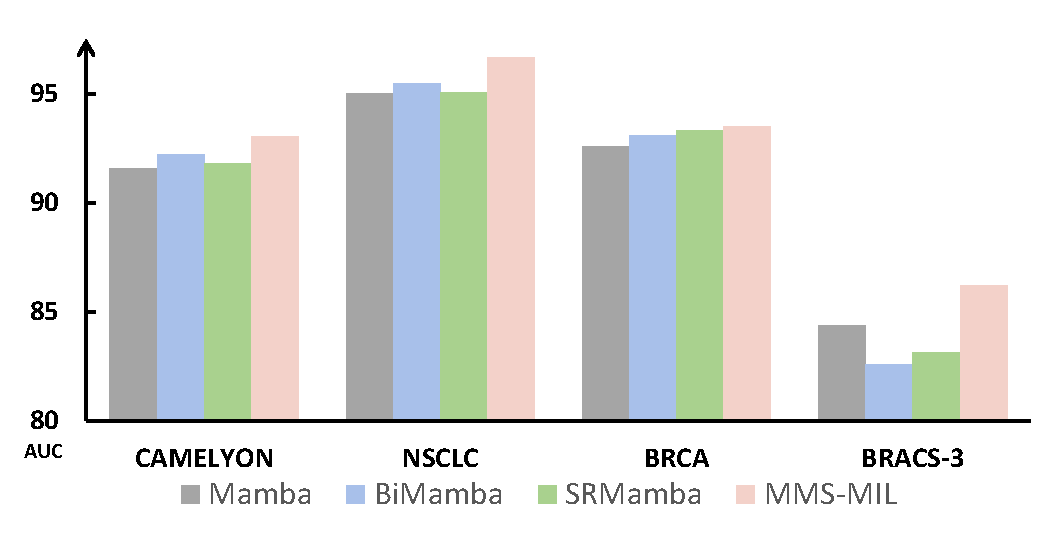
\includegraphics[width=0.9\columnwidth]{figures/MMSMIL的不同Mamba比较.pdf}
  \bicaption[不同Mamba模型的性能比对柱状图]{不同Mamba模型的性能比对柱状图。}[Bar chart of performance comparison of different Mamba models.]{Bar chart of performance comparison of different Mamba models.}
  \label{figure3: DifferentMamba}
  % \vspace{-4pt}
\end{figure}
\textbf{(2)不同Mamba模型性能比对}



为了进一步验证本章的方法的优越性来源于本章的架构而不是Mamba本身,本章对三种变体进行了比较实验:图\ref{figure3: DifferentMamba}中的Mamba Block、BiMamba和SRMamba。
结果表明,M$^2$S-MIL在所有四个数据集上都取得了最佳性能。
本章的方法不仅在性能上超过了原始的单分支Mamba,而且在与没有引入局部连续性和旋转不变性等视觉图像的聚合方法(例如,BiMamba和SRMamba)的比较中表现出许多优势。
实验结果表明,本章的引入2D特性的Mamba比其他多扫描综合的Mamba算法具有更强的实例建模能力,更强的空间信息捕获能力,能够提取更多的判别性特征。



\textbf{(3)讨论区域数量对模型性能的影响}

\begin{figure}[ht]
  \centering
  \captionsetup{font={small, stretch=1.312}}
  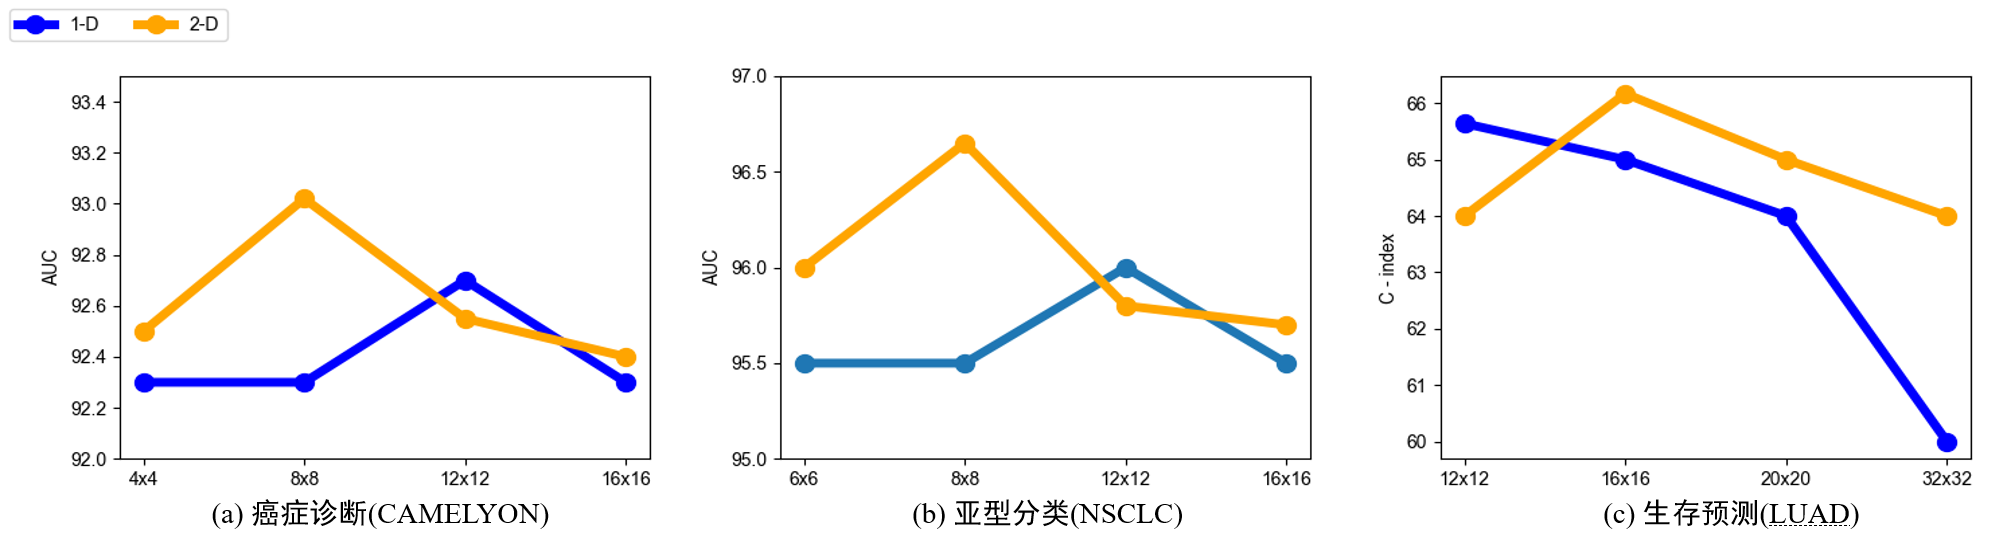
\includegraphics[width=1.0\columnwidth]{figures/区域个数.png}
  \bicaption[不同区域数量的模型性能折线图]{不同区域数量的模型性能折线图。}[Breakpoint plots of model performance for different number of regions]{Breakpoint plots of model performance for different number of regions.}
  \label{figure3: NumOfRegion}
\end{figure}

本小节系统地研究了不同区域划分策略在本章的方法中的影响。图~\ref{figure3: NumOfRegion}展示了不同区域划分在病理分类任务上的性能效果,其中1-D代表并不将之重塑为2D特征图而只进行一维序列的分区。
从与1D的对比实验可以看出,二维区域划分方式优于一维区域划分方式,因为它保留了更多的原始图像的空间信息。
并且本章认为,本章的性能提升并不仅仅依赖于对序列简单的划分区域,侧面印证了本章方法,通过引入更多空间信息从而提高了模型性能。
此外,另一个现象是,使用过小或过大的区域会使性能下降。这是因为小区域大幅降低了Mamba建模二维关系的能力(近似正常原始序列输入),而过大的区域将原本相距较远不具备连续性的特征关联在一起导致性能损耗。
因此,采用适中的区域划分是多扫描Mamba输入的最佳选择。


\textbf{(4)窗口大小对2D 空间上下文感知模块的影响分析}

\begin{table}[h!]
  \large    % 设置表格字体为5号
  \setstretch{1.245}        % 设置具有指定弹力的橡皮长度(原行宽的1.2倍)
  \captionsetup{font={small, stretch=1.512}}
  \centering
  % \vspace{-10pt}
  \bicaption[不同大小窗口对性能影响]{不同大小窗口对性能影响。最优结果用粗体表示。}{Effect of different window sizes on performance. The best results are shown in bold.}    % 中英文标题
  \begin{tabularx}{\textwidth}{lCCCC}
    \toprule
    方法 & CAMELYON& NSCLC&BRCA&BRACS3\\ \midrule
    W/o  & 92.72$\pm$1.82 &  96.25$\pm$1.44 & 93.01$\pm$1.82 &  85.24$\pm$0.32\\
    3 $\times$ 3  &  92.78$\pm$1.52 & 96.31$\pm$1.33 & 93.37$\pm$1.93 & 85.71$\pm$1.80\\
  \textbf{5 $\times$ 5} &\textbf{93.02$\pm$1.20} &\textbf{96.65$\pm$1.08}  &\textbf{93.50$\pm$1.70} & \textbf{86.21$\pm$0.46}\\
    \bottomrule
  \end{tabularx}
  % \vspace{-25pt}
  \label{table3: size of window}
\end{table}

本小节探究了不同窗口大小的2D空间上下文感知模块对M$^2$S-MIL的性能影响。
可以看到越大窗口范围可以整合更多的空间信息,所带来的性能提升越大。
但是由于计算窗口注意力所需要的计算资源随窗口大小增大而增大,所以平衡计算资源与性能之间选择适中的窗口大小是M$^2$S-MIL的最佳选择。

\textbf{(5)使用PLIP作为特征提取器的性能结果}

\begin{table}[h!]
  \large    % 设置表格字体为5号
  \setstretch{1.245}        % 设置具有指定弹力的橡皮长度(原行宽的1.2倍)
  \captionsetup{font={small, stretch=1.512}}
  \centering
  % \vspace{-10pt}
  \bicaption[M$^2$S-MIL以PLIP为离线特征提取器的亚型分型性能]{M$^2$S-MIL以PLIP为离线特征提取器的癌症诊断性能。最优结果用粗体表示,次优结果用下划线表示。}{Cancer diagnosis performance of M$^2$S-MIL with PLIP as the offline feature extractors. The optimal experimental results are marked in bold, and the sub-optimal are underlined.}    % 中英文标题
  \begin{tabularx}{\textwidth}{clCCC}
    \toprule
    &方法  & Accuracy& AUC&F1 - score\\ \midrule
    \multirow{5}{*}{\rotatebox{90}{PLIP}}&AB - MIL  & 90.09$\pm$1.63 & \underline{94.55$\pm$1.91} & 86.48$\pm$2.50\\
    &OriginMamba        & 90.87$\pm$1.52 & 94.44$\pm$2.19 & 87.78$\pm$1.89\\
    &BiMamba          & 90.54$\pm$1.89 & 94.20$\pm$1.99 & 86.82$\pm$2.77\\
    &SRMamba & \underline{91.87$\pm$0.85} & 94.20$\pm$2.16 & \underline{88.37$\pm$1.31}\\
    &\textbf{M$^2$S - MIL}        & \textbf{92.21$\pm$0.60}     & \textbf{95.24$\pm$1.85}      & \textbf{89.46$\pm$0.93}\\  
    \bottomrule
  \end{tabularx}
  % \vspace{-25pt}
  \label{table3: CAMELYON_PLIP}
\end{table}

\begin{table}[h!]
  \large    % 设置表格字体为5号
  \setstretch{1.245}        % 设置具有指定弹力的橡皮长度(原行宽的1.2倍)
  \captionsetup{font={small, stretch=1.512}}
  \centering
  % \vspace{-10pt}
  \bicaption[M$^2$S-MIL以PLIP为离线特征提取器在TCGA-NSCLC上的亚型分型性能]{M$^2$S-MIL以PLIP为离线特征提取器在TCGA-NSCLC上的亚型分型性能。最优结果用粗体表示,次优结果用下划线表示。}{Cancer sub-typing performance of M$^2$S-MIL on the TCGA-NSCLC dataset with PLIP as the offline feature extractors. The optimal experimental results are marked in bold, and the sub-optimal experimental results are underlined.}    % 中英文标题
  \begin{tabularx}{\textwidth}{clCCC}
    \toprule
    &方法  & Accuracy& AUC&F1 - score\\ \midrule
    \multirow{5}{*}{\rotatebox{90}{PLIP}}&AB - MIL  & 89.94$\pm$1.84 & 94.45$\pm$1.64 & 89.43$\pm$1.97\\
    &OriginMamba        & \underline{90.89$\pm$1.60} & 95.57$\pm$1.60 & \underline{90.24$\pm$1.84}\\
    &BiMamba          & 90.70$\pm$1.95 & 95.42$\pm$1.68 & 89.94$\pm$2.26\\
    &SRMamba &  89.85$\pm$2.07 &  \underline{95.72$\pm$1.51} & 88.96$\pm$2.66 \\
    &\textbf{M$^2$S - MIL}        & \textbf{91.56$\pm$1.76}     & \textbf{96.22$\pm$1.12}      & \textbf{90.64$\pm$1.86}\\   
    \bottomrule
\end{tabularx}

  \label{table3: NSCLC_PLIP}
\end{table}


\begin{table}[h!]
  \large    % 设置表格字体为5号
  \setstretch{1.245}        % 设置具有指定弹力的橡皮长度(原行宽的1.2倍)
  \captionsetup{font={small, stretch=1.512}}
  \centering
  % \vspace{-10pt}
  \bicaption[M$^2$S-MIL以PLIP为离线特征提取器在TCGA-BRCA上的亚型分型性能]{M$^2$S-MIL以PLIP为离线特征提取器在TCGA-BRCA上的亚型分型性能。最优结果用粗体表示,次优结果用下划线表示。}{Cancer sub-typing performance of M$^2$S-MIL on the TCGA-BRCA dataset with PLIP as the offline feature extractors. The optimal experimental results are marked in bold, and the sub-optimal experimental results are underlined.}    % 中英文标题
  \begin{tabularx}{\textwidth}{clCCC}
    \toprule
    &方法  & Accuracy& AUC&F1-score\\ \midrule
    
  \multirow{5}{*}{\rotatebox{90}{PLIP}}&AB-MIL  & 83.81$\pm$3.72 & 90.18$\pm$2.99 & 67.94$\pm$4.22\\
  &OriginMamba        & 86.75$\pm$5.76 & \underline{92.90$\pm$2.44} & \underline{74.35$\pm$7.23}\\
  &BiMamba          & \underline{87.73$\pm$3.06} & 92.64$\pm$2.28 & 74.07$\pm$4.75\\
  &SRMamba & 86.40$\pm$3.31 & 92.17$\pm$2.67 & 72.39$\pm$4.62\\
  &\textbf{M$^2$S-MIL}        & \textbf{88.82$\pm$3.22}     & \textbf{93.40$\pm$1.24}      & \textbf{75.00$\pm$2.50}\\  
  \bottomrule
\end{tabularx}
  \label{table3: BRCA_PLIP}
\end{table}





为了进一步探索本章方法的有效性,本小节还进行了将同样采用自监督预训练的PLIP~\cite{huang2023visual}作为特征提取器的相关实验,以验证本章方法的普遍性。
如表\ref{table3: CAMELYON_PLIP}、\ref{table3: NSCLC_PLIP}和表\ref{table3: BRCA_PLIP}所示,可以看出实验结果与R50特征一致。
本章的方法优于其他基于Mamba的方法。在CAMELYON数据集上,它在Accuracy、AUC和F1-score方面分别比次优的方法提高了0.34\%、0.69\%和1.09\%。这些数据在NSCLC数据集中分别为0.57\%,0.4\%和0.4\%。
最后,BRCA数据集的改进也值得注意,Accuracy提高了1.09\%,AUC提高了0.5\%,F1-score提高了0.65\%。
这进一步表明,即使使用非传统的ResNet-50特征提取器,本章方法的性能改进也不仅仅是依赖于简单的多个Mamba分支合并,而是正确捕获了空间信息与视觉特征。


\begin{figure}[ht]
  \centering
  \captionsetup{font={small, stretch=1.312}}
  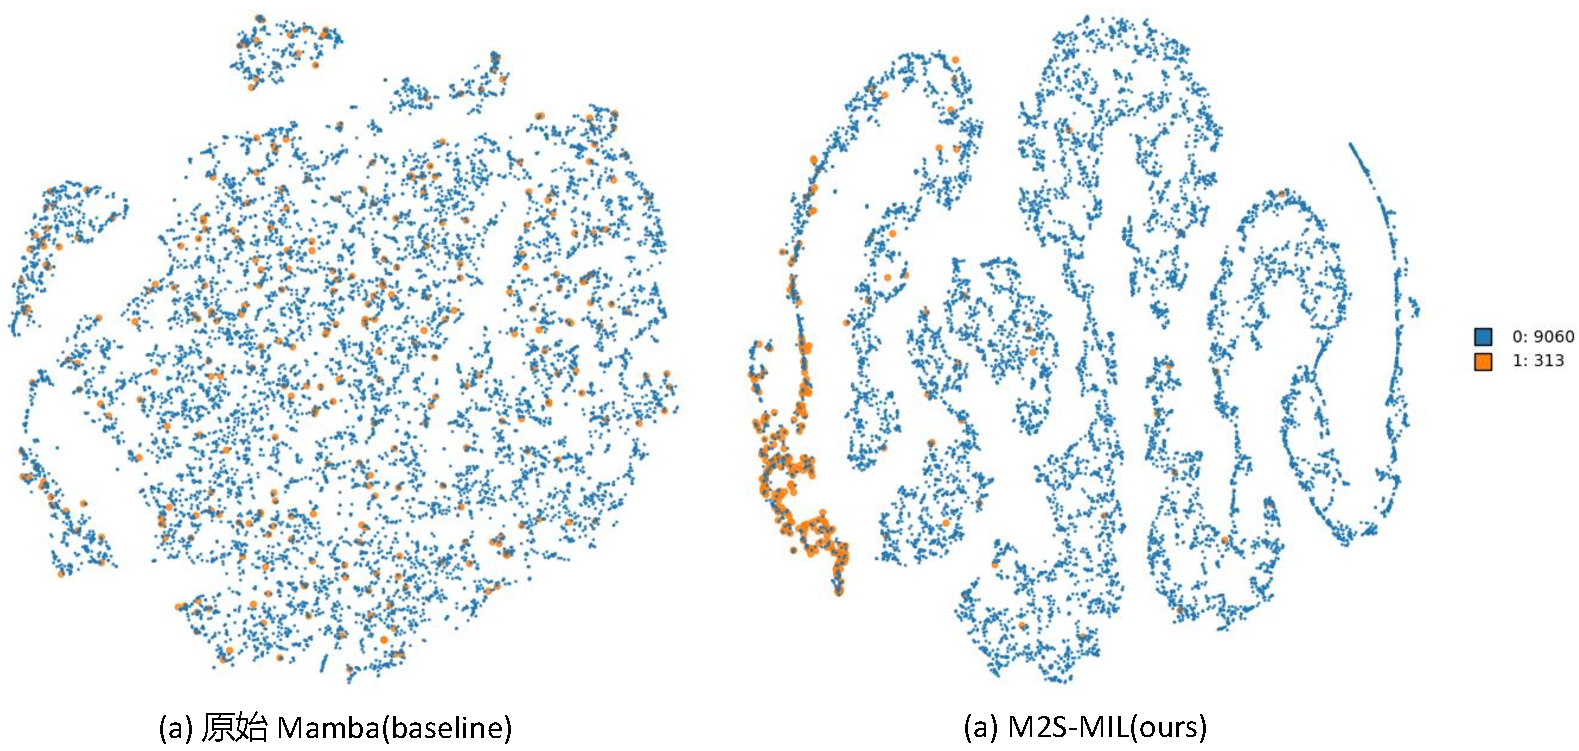
\includegraphics[width=1.0\columnwidth]{figures/vis2_2.pdf}
  \bicaption[原始Mamba(baseline)和M$^2$S-MILL聚合特征t-SNE可视化结果]{原始Mamba(baseline)和M$^2$S-MIL聚合特征t-SNE可视化结果。}[The t-SNE visualization of aggregated features from original Mamba(baseline) and SMC-MIL]{The t-SNE visualization of aggregated features from Mamba(baseline) and SMC-MIL.}
  \label{figure3: tSNE}
\end{figure}

\subsection[\hspace{-2pt}可视化分析]{{\heiti\zihao{4} \hspace{-8pt}可视化分析}}\label{section3: 可视化分析}
\begin{figure}[h!]
  \centering
  \captionsetup{font={small, stretch=1.312}}
  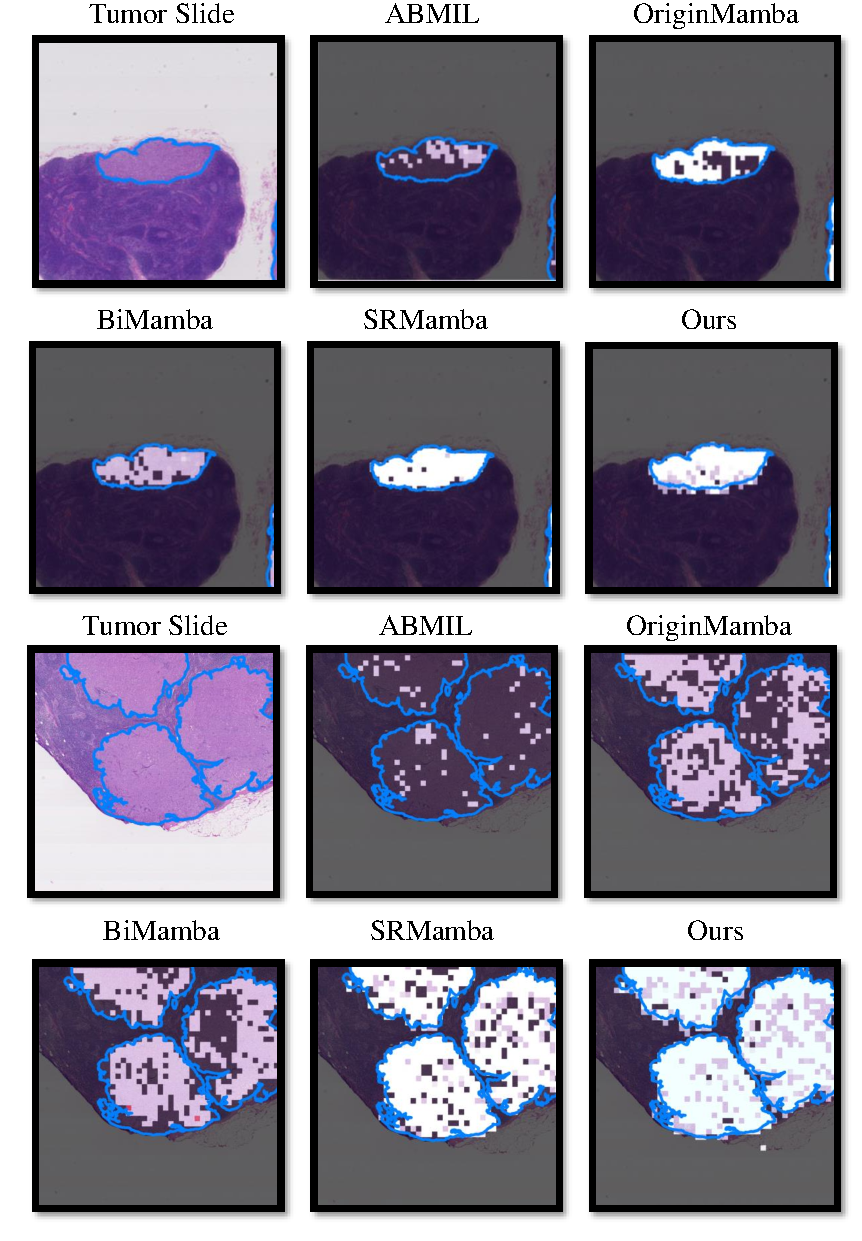
\includegraphics[width=0.7\columnwidth]{figures/vis2.pdf}
  \bicaption[多个Mamba变体和M$^2$S-MIL关注的图块可视化结果]{多个Mamba变体和M$^2$S-MIL关注的图块可视化结果}[Visualization results of patches focused by other Mamba and SMC-MIL]{Visualization results of patches focused by other Mamba variants(baseline) and SMC-MIL.}
  \label{figure3: visualize}
\end{figure}

为了直观地验证本章方法的可解释性,本章用t-SNE可视化了同一个WSI切片的所有实例经过Mamba和M$^2$S-MIL所建模出后的特征,结果展示在图\ref{figure3: tSNE}。
可以看到M$^2$S-MIL更具有条理,而原始Mamba的结果更为混乱。说明M$^2$S-MIL使Mamba的实例间的关系建模能力更为出色。

并且本章将多种Mamba变体与本章的方法在Camelyon-16数据集上产生的高注意力分数的实例可视化,如图\ref{figure3: visualize}所示。
蓝色的线条勾勒出肿瘤区域。越亮的斑块表明注意力得分越高。
可视化结果清楚地表明,与原始Mamba相比,M$^2$S-MIL能够更准确地选择显著斑块。
 

\section[\hspace{-2pt}本章小结]{{\heiti\zihao{-3} \hspace{-8pt}本章小结}}\label{section3: 本章小结}

本章针对序列关系建模模型Mamba在处理数字病理图像分类任务时,对视觉任务特性和空间关系捕捉不充分的问题,
提出了一种简单有效的解决思路,并提出一种新的多实例学习方法:
基于空间信息增强的多扫描Mamba的数字病理图像分类(Multi-scan Mamba with Sptial information enhancement,简称M$^2$S-MIL)。
该方法通过综合多种扫描模式的信息,针对病理图像空间信息,设计了区域螺旋扫描和网格扫描模式,增强Mamba对病理图像空间关系的建模。
同时利用2D空间上下文感知模块,进一步对整合后的序列进行空间关系增强,提升模型性能。
在3个WSI子任务以及7个数据集上的大量对比及消融实验充分证明了,本章提出的基于空间信息增强的多扫描Mamba的多实例学习架构综合了多种扫描模式分支,
引入空间信息,解决了数字病理图像分类任务中使用Mamba模型存在的图像空间结构捕获能力不足的问题。
%未来,作者将计划进一步探索如何在更有限的扫描模式序列情况下,使Mamba更高效更好地捕获空间关系,更充分建模实例间关系。
\chapter[\hspace{0pt}基于扫描不变性Mamba的高分辨率病理图像分类研究]{{\heiti\zihao{3}\hspace{0pt}基于扫描不变性Mamba的高分辨率病理图像分类研究}}\label{chapter4: 基于扫描不变性Mamba的高分辨率病理图像分类研究}
\removelofgap
\removelotgap

上一章研究了基于多扫描Mamba的高分辨率病理图像分类算法,在保留Mamba高效的建模能力同时,通过引入2D图像空间结构信息,增强Mamba对实例间空间结构关系的建模能力,并且通过集成多扫描分支的方式缓解了Mamba对顺序的依赖,提高了模型性能。
然而,该算法仅关注于输出序列信息的整合,未能从根本上突破序列输入顺序对Mamba建模能力的约束,仅仅是一种妥协的策略,依旧高度依赖扫描模式与集成方式。
因此,在上一章的基础上,本章主要研究基于扫描不变性Mamba的高分辨率病理图像分类算法,通过构建成对的差异化实例序列,并在此基础上开展对比学习,促进Mamba模型忽略序列顺序,挖掘并聚合关键实例特征。
本章内容共分为四节,\hyperref[section4: 研究动机]{第一节}介绍本章的研究动机;\hyperref[section4: 基于序列差异化对比的Mamba模型]{第二节}介绍本章提出的基于扫描不变性Mamba的高分辨率图像分类算法;
\hyperref[section4: 实验设置及结果分析]{第三节}给出实验设置和结果分析;\hyperref[section4: 本章小结]{第四节}对本章进行小结。


%\subsection[\hspace{-2pt}研究动机]{{\heiti\zihao{4} \hspace{-8pt}研究动机}}\label{section4: 研究动机}

\section[\hspace{-2pt}研究动机]{{\heiti\zihao{-3} \hspace{-8pt}研究动机}}\label{section4: 研究动机}

在经典的MIL范式中,使用预训练模型将实例转化成离线特征,然后聚合成包级别的特征表示,以进行后续分析。
在这个范式中,由于病理图像的高分辨率特性,导致其划分后的实例数目过多,因此WSI分类可以被视为一个长序列建模问题,通过将包中的大量实例视为标记来处理,能够建模实例与整个包之间的空间上下文相关性,以捕捉判别性信息。
一些基于状态空间模型(State Space Model,SSM)的方法被设计来有效对长序列进行建模。
Mamba是最近提出的一种具有代表性的基于SSM架构的模型,与ViT相比具有更好的长序列建模性能,但需要的计算资源更少~\cite{zhu2024vision}。
然而,在Mamba模型和MIL任务之间存在一个根本的区别:如图~\ref{figure1: Mamba模型与MIL任务差异}所示,Mamba作为扫描序列敏感模型,其性能高度依赖实例的输入顺序,这与多实例学习的序列不变性要求存在本质冲突,导致模型在病理图像分类任务中易受随机序列干扰而产生性能波动。

为了调和扫描敏感的Mamba和扫描不变的MIL之间的差异,以前的工作包括上一章的方法都主要是将不同扫描模式的图像Patch序列输入到Mamba中,然后将多个输出序列聚合。
例如,MamMIL~\cite{fang2024mammil}结合了Bi-SSM和2D-CAB模块以整合来自原始序列、反向序列和局部序列的扫描模式信息。
而MambaMIL~\cite{yang2024mambamil}将序列重塑为矩形,并应用序列重新排序操作来垂直扫描新序列。
然而,用于生成实例序列的扫描模式数量有限,限制了模型对扫描模式不变特征的学习能力。
因此,这并没有从根本上减轻扫描模式对Mamba性能的影响,仅仅是一种妥协的策略,其依旧高度依赖扫描模式和集成形式。


\section[\hspace{-2pt}基于序列差异化对比的Mamba模型]{{\heiti\zihao{-3} \hspace{-8pt}基于序列差异化对比的Mamba模型}}\label{section4: 基于序列差异化对比的Mamba模型}

\subsection[\hspace{-2pt}方法概述]{{\heiti\zihao{4} \hspace{-8pt}方法概述}}\label{section4: 方法概述}
%为了解决这个问题,本章提出了一种新的MIL框架,称为扫描不变Mamba对比学习(SMC-MIL),它使Mamba能够学习实例序列的扫描不变包特征,从而协调扫描敏感Mamba和基于扫描不变MIL的WSI分类任务之间的差异。具体来说,为了消除扫描敏感Mamba在MIL任务中引入的偏差,本章设计了一个对比学习目标,以强制在两个极端不同的扫描序列之间通过相同的Mamba获得的包表示和分类逻辑的一致性。本文提出了一种基于实例评估的序列增强方法,该方法通过一系列的序列增强和掩蔽来扩大序列排列、序列长度的多样性,以及从序列中获得判别性区域的难度。该方法增加了对比学习的难度,并强制Mamba在输入序列差异极大的情况下学习对WSI图像的一致表示和决策,从而赋予了Mamba良好的扫描不变建模和判别实例识别能力。在许多计算病理学任务上进行的大量实验验证了本章的方法优于其他现有方法。

虽然Mamba在实例特征学习和对大包(长序列)的处理效率上具有突出的优势,但它是扫描敏感的,这与MIL的假设不一致。
在MIL中,Mamba的输出不应该依赖于实例输入顺序,也不应该对实例数量敏感。
换句话说,MIL对于实例输入是扫描不变的。在这种情况下,本章精心设计了一个基于对比学习的扫描不变Mamba模型,旨在更好地将先进的Mamba模型适应于MIL任务。

如图~\ref{figure3: SMCMIL}所示,本章的模型由两个Mamba分支组成。一个是“Easy”的分支,而另一个是“Hard”的分支。
在“Easy”分支中,对高度关注的实例通过Mixup生成越来越多的突出实例,从而降低包分类的难度。
而在“Hard”分支中,将容易分类的实例进行掩码,以提高包分类的难度。
显然,这两个分支在扫描顺序、实例数目和包分类难度上存在较大差异。
因此,本章方法采用对比学习强制Mamba对这两个不同序列输出相同的结果,从而赋予Mamba这样一个扫描不变的属性。
此外,极高的分支差异也使得Mamba通过对比学习进一步增强了泛化能力。

本研究的主要贡献可以概括为以下几点:
\begin{itemize}
  \item 本研究提出了一个基于Mamba的多实例学习框架,命名为SMC-MIL,用于计算病理学。SMC-MIL通过实例序列对比学习来引导Mamba学习扫描不变的包表示,这更适合基于MIL的WSI分类范式。
  \item 设计了一个双分支实例序列对比学习框架,旨在实现两个极端不同的输入实例序列之间的一致性,消除序列排列对最终包决策的影响。该框架为使用SSM处理MIL任务提供了一个简单而有效的解决方案。
  \item 提出了一种序列对比度增强方法,该方法基于实例分类困难程度的评估,而有意地打乱、增强和掩盖实例。该方法不仅增加了两个输入对比序列在顺序和长度上的差异,而且扩大了识别判别区域的难度差异。显然,这种方法增加了对比学习的难度,从而迫使Mamba在不考虑其图块序列排列的情况下学习WSI的判别特征。 
\end{itemize}

\begin{figure}[h]
  \centering
  \captionsetup{font={small, stretch=1.312}}
  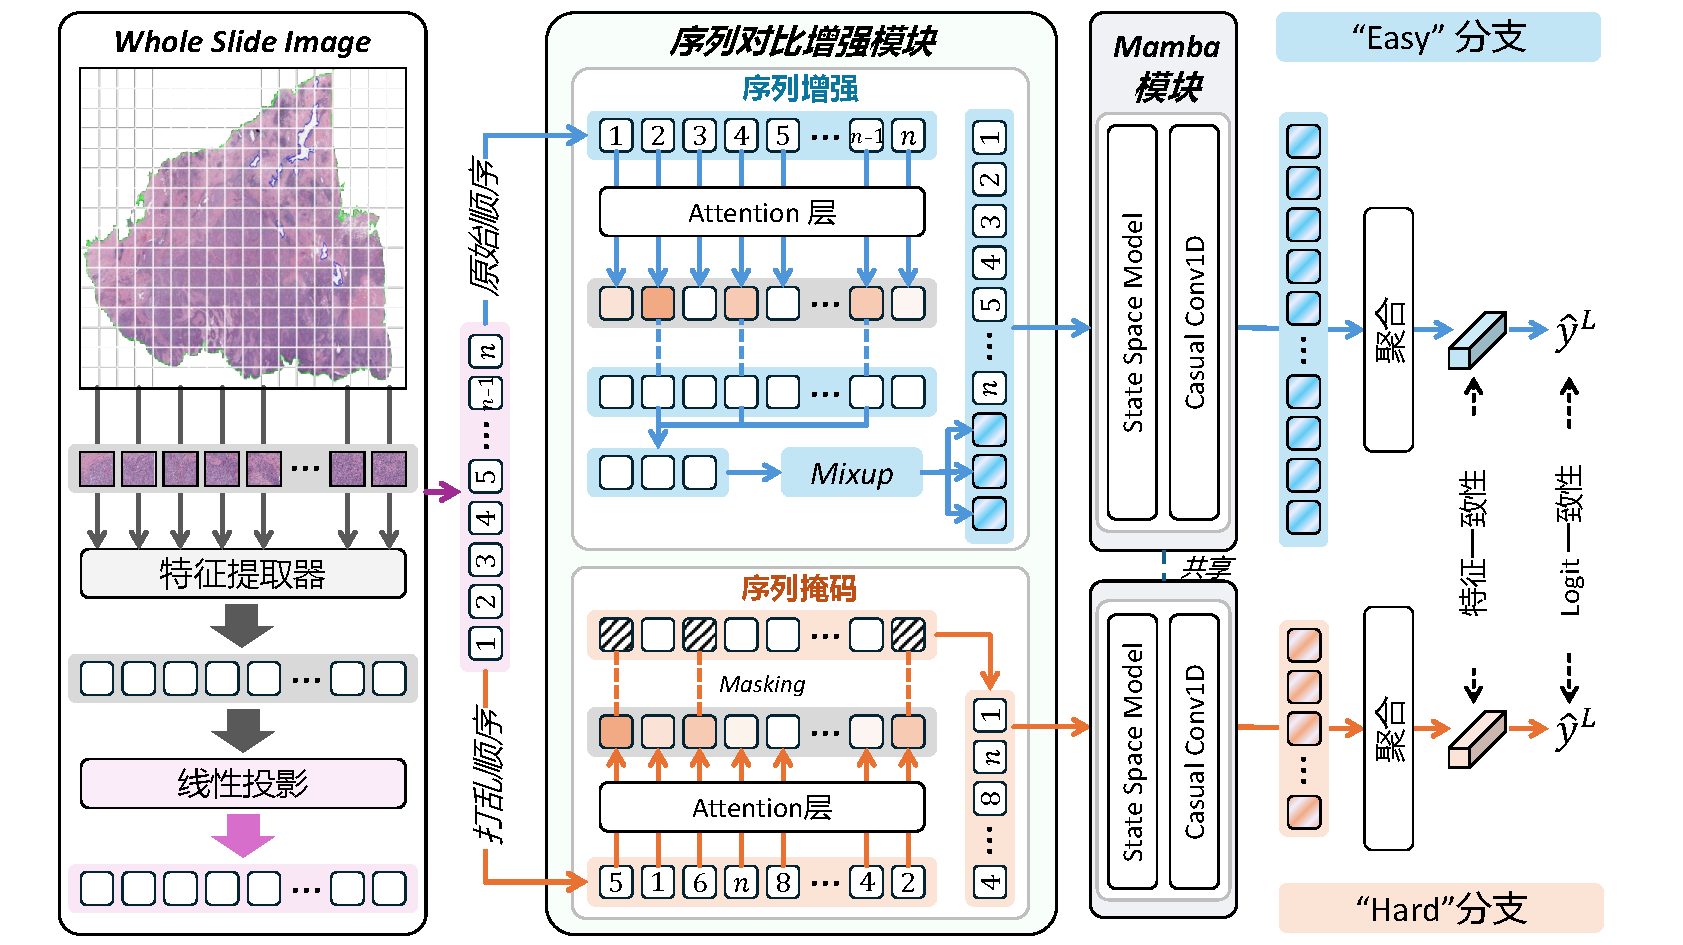
\includegraphics[width=1.0\columnwidth]{figures/SMCMIL.pdf}
  \bicaption[SMC-MIL模型总览图]{SMC-MIL模型总览图。}[Overview of proposed SMC-MIL]{Overview of proposed SMC-MIL.}
  \label{figure3: SMCMIL}
\end{figure}

\subsection[\hspace{-2pt}预处理与特征提取]{{\heiti\zihao{4} \hspace{-8pt}预处理与特征提取}}\label{section4: 预处理与特征提取}

遵从文献~\cite{lu2021data}的设置,每张病理图像被裁剪成一系列$256\times256$的非重叠补丁,放大倍数为$20$倍,同时丢弃背景区域(饱和度$< 15$)。
本章采用ResNet-50~\cite{ROYERCARFAGNI2001253}或UNI~\cite{chen2024towards}作为底层特征提取器$\mathcal{F}(\cdot)$。
因此,本章定义原始扫描序列为:
\begin{equation}
  \mathnormal{Z}=\{z_i\}^{\mathnormal{N}}_{i=1},
\end{equation}
其中$z_i$是$X$的第$i$个实例的提取特征,$N$是实例的个数。
另一个扫描序列定义为$Z'=Resort(Z)$(即$Z'$通过对第一个扫描序列的顺序进行随机重排获得,$Resort(\cdot)$表示随机重排操作)。

\subsection[\hspace{-2pt}基于Mamba的双分支对比架构]{{\heiti\zihao{4} \hspace{-8pt}基于Mamba的双分支对比架构}}\label{section4: 基于Mamba的双分支对比架构}

通过进行序列对比学习,引导Mamba学习扫描不变的包特征。
在该方法中,本章设计了一个双分支实例序列对比学习框架,旨在实现两个极端不同的输入实例序列之间的一致性,并消除序列排列对最终包决策的影响。

假设差异化序列对比增强模块为$S(\cdot)$,则通过差异化序列生成模块可得到两个极端不同的序列:
\begin{equation}
  \begin{aligned} 
    Z_1&=S(Z),\\
    Z_2&=S(Z').
\end{aligned}
\end{equation}
给定一个Mamba模块$\mathrm{\Psi}\left(\cdot\right)$与一个注意力聚合模块$\phi\left(\cdot\right)$,分别对实例序列进行实例关键建模和特征聚合,
为了方便后续表示,该聚合过程记作$\rho\left(\cdot\right)$,统称为Mamba聚合器。
根据上述步骤,则差异化的两个序列分支的包特征分别为:
\begin{equation}
  \begin{aligned} 
  \mathbf{b_1}=\rho(Z_1),\\
  \mathbf{b_2}=\rho(Z_2).
\end{aligned}
\end{equation}

这两个特征都是同一个病理图像的有效表示,因此应该反映一致的视觉内容,本章称之为特征一致性。

给定一个分类器$\mathcal{C}(\cdot)$,分别对这些特征进行分类,获取其分类标签:
\begin{equation}
  \begin{aligned} 
    {\hat{Y}}_1=\mathcal{C}(\mathbf{b_1}),\\
    {\hat{Y}}_l=\mathcal{C}(\mathbf{b_2}).
\end{aligned}
\end{equation}
同样的,这两个标签应该反映一致分类结果,本章称之为标签一致性。

通过特征一致性和标签一致性的约束,反向优化引导Mamba架构学习到与扫描无关的包特征,从根本上突破Mamba架构对输入顺序的依赖,使Mamba架构更适配高分辨率病理图像分类任务。

\subsection[\hspace{-2pt}差异化序列生成(简单与困难分支)]{{\heiti\zihao{4} \hspace{-8pt}差异化序列生成(简单与困难分支)}}\label{section4: 差异化序列生成(简单与困难分支)}

基于扫描序列的顺序、长度以及发现判别区域的难易程度的三个角度,本章提出了一种序列对比度增强方法进行差异化序列生成,即构造“Easy”分支和“Hard”分支。
根据所在分支的不同,上小节提到的序列对比增强模块$S(\cdot)$,可分为两个子模块:序列增强模块$S_A(\cdot)$和序列掩码模块$S_M(\cdot)$。
下面分别详细介绍这两个部分。

\textbf{序列增强 (“Easy” 分支)} 

如图~\ref{figure3: SMCMIL}顶部所示,本章设计了一个基于注意力的序列增强模块来构建“Easy”分支。其核心思想是使用注意力机制识别高关注实例,然后通过Mixup对这些已识别的实例执行实例级增强。
此过程生成新实例来补充原始序列。本章将每个实例的注意力得分定义为:
\begin{equation}
  \mathnormal{A}=[a_1,...,a_i,...,a_N]=\mathnormal{\phi}(\mathnormal{Z}),
  \label{eq8}
  \end{equation}
其中$\mathnormal{\phi}(\cdot)$为注意力模块。然后将其进行排序:
\begin{equation}
  \mathnormal{I}=[i_1,i_2,...,i_N]=Sort(\mathnormal{A}),
  \label{eq9}
  \end{equation}
其中$i_1$为注意力得分最高实例的索引,$i_N$为得分最低实例的索引。
本章将实例的$\alpha\%$作为进行序列增强的实例。
其对应的索引是$\lfloor \alpha\% \times N \rfloor$,其对应的实例注意力分数是$I_h=[i_t]^{\lfloor \alpha\% \times N \rfloor}_{t=1}$。则增强序列可表示为:
\begin{equation}
  \mathnormal{Z_{easy}}\leftarrow S_A(Z):=concat\{\varphi(Z_{\mathnormal{I}_h}),Z\},
  \label{eq10}
  \end{equation}
其中$\varphi(\cdot)$是所选实例上的Mixup操作,$S_A(\cdot)$是序列增强模块,$concat$则代表将进行Mixup后的实例同样拼接到原本实例序列上。
注意,这里的注意力机制与后续聚合模块中的注意力模型共享参数。
因此,在“Easy”分支中输入Mamba的序列长度为$\lfloor \alpha\% \times N \rfloor + N$。

\textbf{序列掩码(“Hard”分支)} 

如图~\ref{figure3: SMCMIL}底部所示,本章采用基于注意力的掩蔽机制来掩盖“Hard”分支中容易区分的实例,迫使Mamba增强其鉴别可判别性区域的能力。对于分类模型,本章认为具有最高和最低关注值的实例是最容易区分的。
因此,本章试图掩盖这些实例,以迫使模型学习更精确的分类边界。具体来说,本章生成一个$n$维掩码向量$M$如下所示:
  \begin{equation}
    \mathnormal{M}=[m_1,...,m_i,...,m_N],
    \label{eq11}
    \end{equation}
其中$m_i \in \{0,1\}$。如果$m_i$ = 1,则第$i$个实例被保留;$m_i$ = 0时,第$i$个实例被掩码。
本章将高关注值和低关注值的掩码率分别设置为$\beta_h\%$ 和 $\beta_l\%$。
那么,高值对应的序列下标为$I_{\beta_h}=[i_t]^{\lfloor \beta_h\%\times N \rfloor}_{t=1}$,低值对应的序列下标为 $I_{\beta_l}=[i_t]^{N}_{t=N-\lfloor \beta_l\%\times N \rfloor}$。因此,
\begin{equation}
  \mathnormal{m_i}=\left \{
  \begin{array}{cl}
      0 &  i\in I_{\beta_h} \cup  I_{\beta_l}, \\
      1 & other.
  \end{array}\right.
  \label{eq12}
  \end{equation}
最后,掩码后的序列可以表示为:
\begin{equation}
  \mathnormal{Z_{hard}}\leftarrow S_M(Z'):=M\cdot \mathnormal{Z'},
  \label{eq13}
  \end{equation}
其中$S_M(\cdot)$是序列掩码模块。为了便于讨论,本文假设$\beta_h=\beta_l$。

“Easy”分支保留了原本的序列顺序,同时增加了序列长度,并且通过Mixup操作添加了多样性,降低了Mamba捕获可判别性区域的难度;
“Hard”分支打乱了原本的序列顺序,同时缩减了序列长度,并且通过掩盖掉易于分辨的实例,提高了Mamba捕获可判别性区域的难度。
上下两个分支形成了鲜明的对比。如此差异化的序列分支,加大了对比学习任务的难度,迫使Mamba学习到更清晰的分类边界,以提高模型鲁棒性。

\subsection[\hspace{-2pt}基于Mamba的实例聚合]{{\heiti\zihao{4} \hspace{-8pt}基于Mamba的实例聚合}}\label{section4: 基于Mamba的实例聚合}
本小节介绍基于Mamba的实例聚合,即上文所提到的Mamba聚合器$\rho\left(\cdot\right)$。
如上所述,“Easy”和“Hard”分支的输入实例序列分别为$\mathnormal{Z_{easy}}$和$\mathnormal{Z_{hard}}$。$\Psi(\cdot)$是上文提到的一个Mamba块。这两个分支的包表示可以通过执行基于注意力机制的聚合来获得,
\begin{equation}
  \begin{aligned}
      &\mathbf{b}_1=\mathnormal{A_1} \cdot \Psi(\mathnormal{Z_{easy}})=\phi(\Psi(S_A(Z)))\cdot \Psi(S_A(Z)), \\
      &\mathbf{b}_2=\mathnormal{A_2} \cdot \Psi(\mathnormal{Z_{hard}})=\phi(\Psi(S_M(Z')))\cdot \Psi(S_M(Z')),
  \end{aligned}
  \label{eq6}
\end{equation}
其中$\mathnormal{A_1}$和$\mathnormal{A_2}$分别是$ \Psi(\mathnormal{Z_{easy}})$和$ \Psi(\mathnormal{Z_{easy}})$的注意力分数。类似地,它们的预测包标签可以通过将包的表示输入分类器$\mathcal{C}(\cdot)$得到,
\begin{equation}
  \begin{aligned}
      &\hat{Y}_1\leftarrow \mathcal{C}(\mathbf{b}_1):=\mathcal{C}(\mathnormal{A_1}\cdot \Psi(\mathnormal{Z_{easy}})),\\
      &\hat{Y}_2\leftarrow \mathcal{C}(\mathbf{b}_2):=\mathcal{C}(\mathnormal{A_2} \cdot \Psi(\mathnormal{Z_{hard}})).
  \end{aligned}
  \label{eq7}
  \end{equation} 

\subsection[\hspace{-2pt}基于一致性的模型优化]{{\heiti\zihao{4} \hspace{-8pt}基于一致性的模型优化}}\label{section4: 基于一致性的模型优化}

由于这两个分支的扫描序列都来自同一个包,因此它们的包表示和分类应该是一致的。它们的包表示的一致性损失为:
\begin{equation}
    \mathcal{L}_{b_{con}}=-%\frac{softmax(\mathbf{b}_1)log(\mathbf{b}_2)+softmax(\mathbf{b}_2)log(\mathbf{b}_1)}{2} , 
    %\frac{1}{2}[\mathrm{Softmax}(\mathbf{b}_1)\log(\mathbf{b}_2)+\mathrm{Softmax}(\mathbf{b}_2)\log(\mathbf{b}_1) ]
    \frac{\mathrm{Softmax}(\mathbf{b}_1)\log(\mathbf{b}_2)+\mathrm{Softmax}(\mathbf{b}_2)\log(\mathbf{b}_1)}{2}.
    \label{eq15}
  \end{equation}
而它们的包分类的一致性损失为:
\begin{equation}
    %\mathcal{L}_{l_{con}}=-(\mathrm{softmax}(\hat{Y}_1)\mathrm{log}(\hat{Y}_2)+\mathrm{softmax}(\hat{Y}_2)\mathrm{log}(\hat{Y}_1))/2.
    %\mathcal{L}_{l_{con}}=-\frac{1}{2}[\mathrm{Softmax}(\hat{Y}_1)\log(\hat{Y}_2)+\mathrm{Softmax}(\hat{Y}_2)\log(\hat{Y}_1)].
    \mathcal{L}_{l_{con}}=-\frac{\mathrm{Softmax}(\hat{Y}_1)\log(\hat{Y}_2)+\mathrm{Softmax}(\hat{Y}_2)\log(\hat{Y}_1)}{2}.
    \label{eq16}
  \end{equation}
除了一致性损失之外,本章还向“Easy”分支引入了分类损失,以确保预测标签与其真实值之间的一致性,
\begin{equation}
	\mathcal{L}_{cls}=Y \log\hat{Y}_1+(1-Y)\log(1-\hat{Y}_1),
	\label{eq14}
\end{equation}
其中$Y$是真实值。
综上所述,该模型可通过处理以下优化问题得到:
\begin{equation}
	\{\hat{\Psi},\hat{\phi},\hat{\mathcal{C}}\}\leftarrow \arg\mathop{\min}\limits_{\hat{\Psi},\hat{\phi},\hat{\mathcal{C}}} \mathcal{L}=\mathcal{L}_{cls}+\gamma (\mathcal{L}_{b_{con}}+\mathcal{L}_{l_{con}}),
	\label{eq17}
\end{equation}
其中$\hat{\Psi},\hat{\phi},\hat{\mathcal{C}}$是本章网络的参数,$\gamma$是平衡分类损失和一致性损失的参数。

\subsection[\hspace{-2pt}模型推理]{{\heiti\zihao{4} \hspace{-8pt}模型推理}}\label{section4: 模型推理}

在模型训练阶段,本章采用双分支对比学习架构,通过约束其中特征一致性和标签一致性,反向梯度优化Mamba架构。
而在模型推理环节,本章仅借助单分支 Mamba 模型来执行图像的标签预测工作。详细来讲,本章分别对以下两种推理模式进行了尝试:


\begin{figure}[h]
  \centering
  \captionsetup{font={small, stretch=1.312}}
  \subfloat[采用序列增强模块进行推理]{
		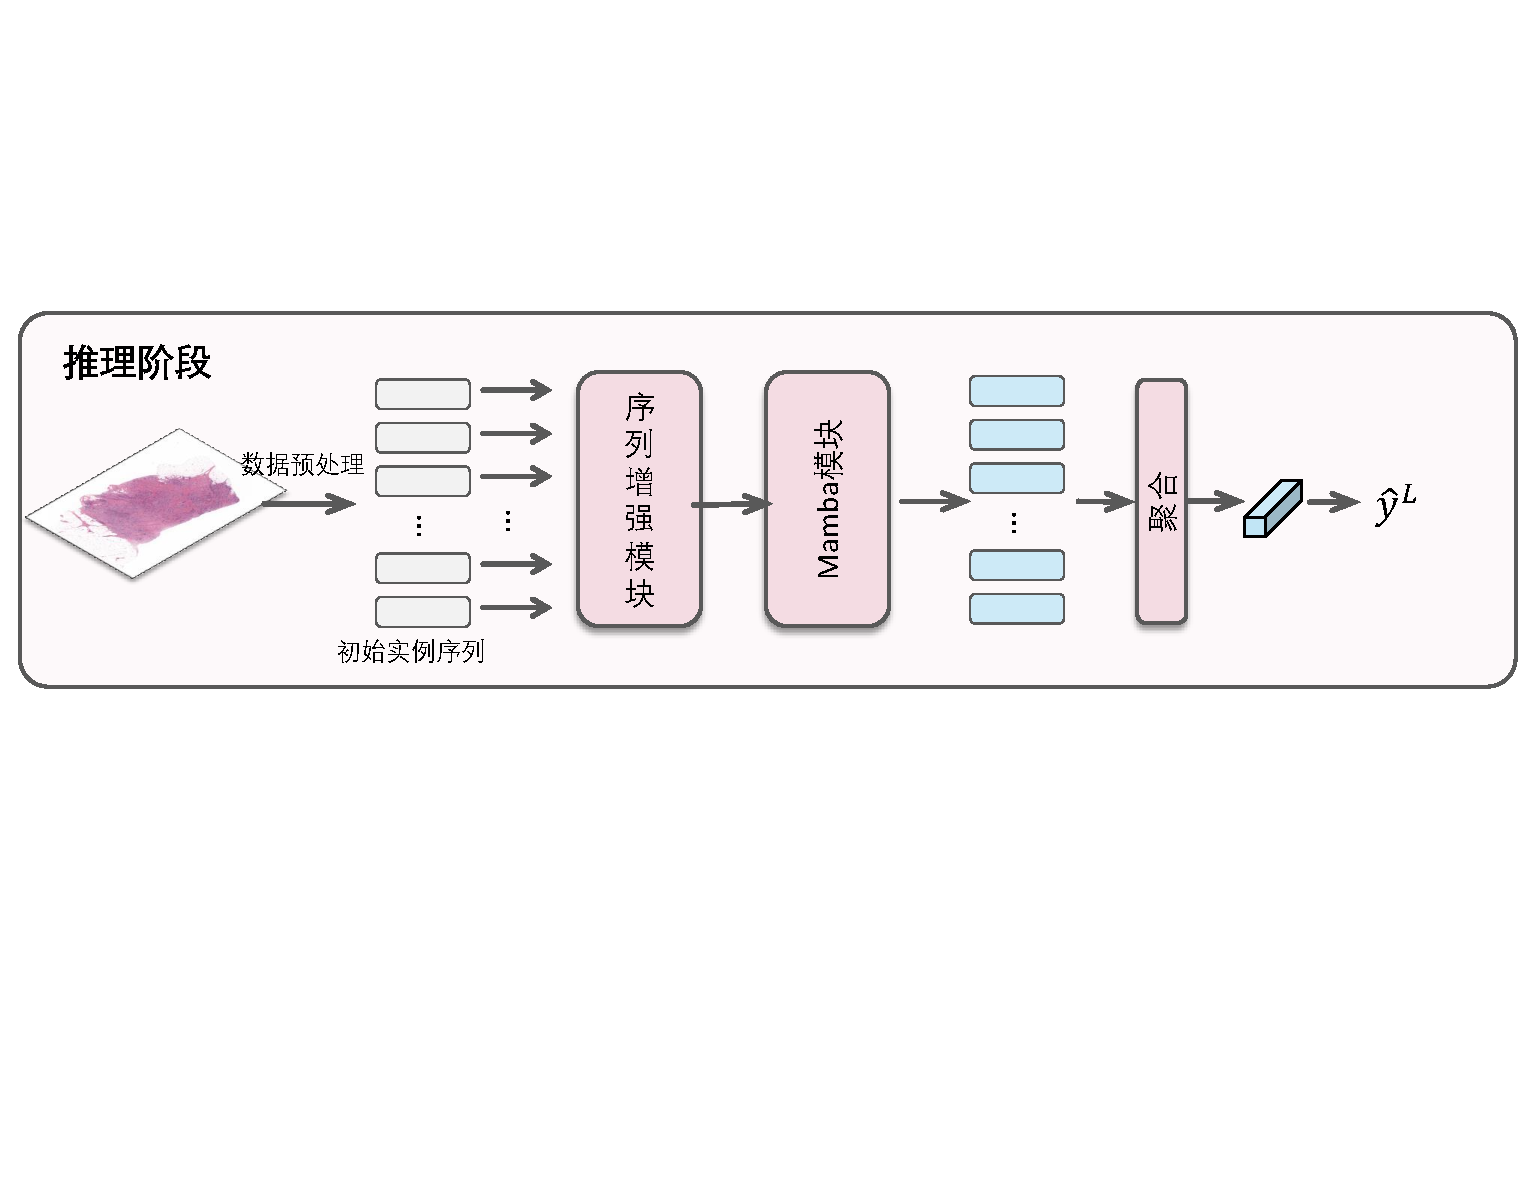
\includegraphics[width=1.0\columnwidth]{figures/基于easy分支的推理阶段.pdf}
    \label{figure3:推理流程1}
    }\\
  \subfloat[不采用序列增强模块进行推理]{
		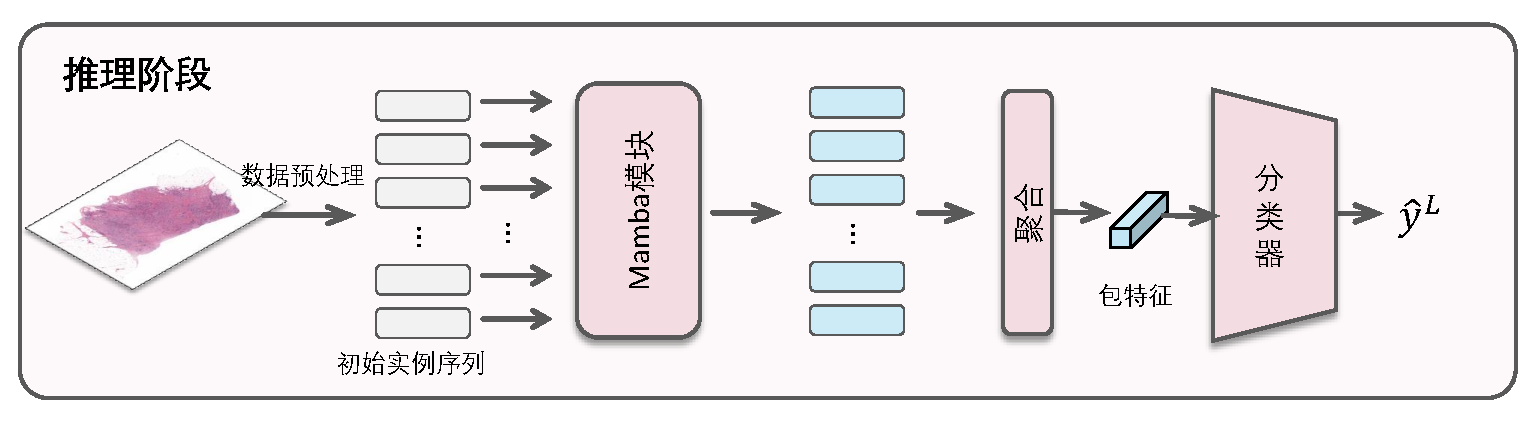
\includegraphics[width=1.0\columnwidth]{figures/基于Mamba的推理阶段.pdf}
    \label{figure3:推理流程2}
    }
  %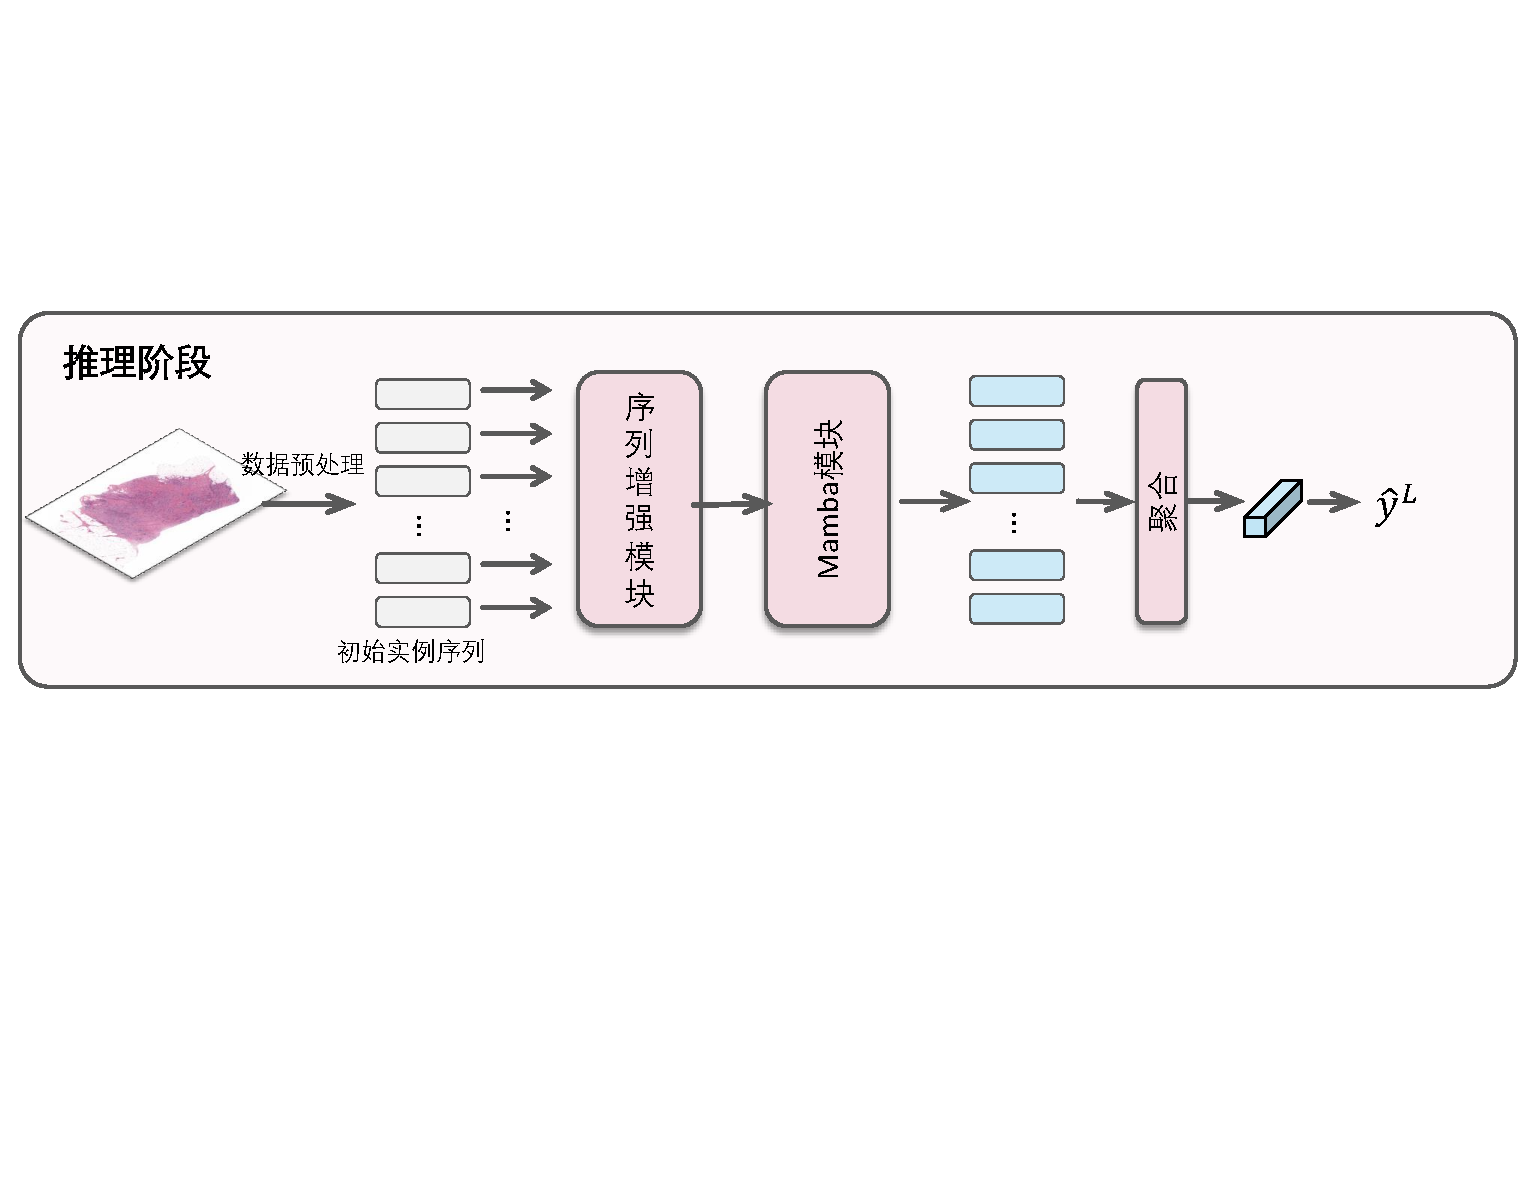
\includegraphics[width=1.0\columnwidth]{figures/基于easy分支的推理阶段.pdf}
  \bicaption[SMC-MIL模型推理流程示意图]{SMC-MIL模型推理流程示意图。}[Schematic diagram of SMC-MIL model inference process]{Schematic diagram of SMC-MIL model inference process.}
  \label{figure3: 推理流程}
\end{figure}

\textbf{采用序列增强模块进行推理:} 给定一张图像$X$经过图像预处理操作后得到实例特征序列,送入到序列增强模块获得新的序列。
继续送入Mamba模块后建模各实例间信息,建模出更好的特征。
最终,通过聚合模块输出包特征,将其输入分类网络以生成最终预测结果。
具体推理流程详见图~\ref{figure3:推理流程1}。

\textbf{不采用序列增强模块进行推理:} 本章还尝试了不采用序列增强模块直接进行输入至Mamba模块进行推理。推理流程详情见图~\ref{figure3:推理流程2}所示。

在不特别说明的情况下,本文采用序列增强模块进行推理。

\section[\hspace{-2pt}实验设置及结果分析]{{\heiti\zihao{-3} \hspace{-8pt}实验设置及结果分析}}\label{section4: 实验设置及结果分析}

在本节中,首先介绍了本章方法的实验设置,包括实验使用数据集、评估指标和实验细节,
然后分析了基于扫描不变性Mamba的高分辨率病理图像分类实验结果,接下来对模型的各个模块以及超参数进行了消融实验和分析,最后对模型所关注的重点区域进行了可视化分析。

\subsection[\hspace{-2pt}实验设置]{{\heiti\zihao{4} \hspace{-8pt}实验设置}}\label{section4: 实验设置}
\textbf{(1)实验环境}


本章实验依托于和上一章实验同样的设置环境和平台。该平台搭载AMD Ryzen 5700X 20 核中央处理器与 3 块 NVIDIA RTX 3090 图形处理器。
实验框架基于 Python 编程语言构建,采用 OpenSlide 库实现病理图像的高效读取,基于 Matplotlib 库完成数据可视化。
详细的实验环境参数配置见表~\ref{table4: env}:

\begin{table}[h!]
  \small    % 设置表格字体为5号
  \setstretch{1.245}        % 设置具有指定弹力的橡皮长度(原行宽的1.2倍)
  \captionsetup{font={small, stretch=1.512}}
  \centering
  \bicaption[基于扫描不变性Mamba的高分辨率病理图像分类研究的实验环境及配置 ]{基于扫描不变性Mamba的高分辨率病理图像分类的实验环境及配置}[Experimental environment and configuration of SMC-MIL ]{Experimental environment and configuration of SMC-MIL}
  \begin{tabularx}{\textwidth}{CcCC}
  \toprule
  设备     & 配置               & 版本          & 数量 \\ 
  \midrule
  操作系统   & Ubuntu           & 20.04.4 LTS & 1  \\
  CPU    & AMD Ryzen 5700X  & -           & 1  \\
  GPU    & GeForce RTX 3090 & -           & 3  \\
  IDE    & VsCode           & 1.86.2      & 1  \\
  编程语言   & Python           & 3.10.11       & -  \\
  深度学习框架 & Pytorch          & 2.0.1       & -  \\
  \bottomrule
  \end{tabularx}
  \label{table4: env}
  \end{table}


\textbf{(2)数据集}

本章通过三个WSI分析子任务来评估SMC-MIL模型:癌症诊断、亚型分类和生存预测。
对于癌症诊断任务,本章采用和上一章同样的设置,采用CAMELYON数据集进行评估。
对于分型任务,本章使用 TCGA-NSCLC、TCGA-BRCA和BRACS~\cite{brancati2022bracs}数据集。
同时为了评估生存预测的准确性,本章使用 TCGA-LUAD,TCGA-LUSC,TCGA-BLCA来评估生存预测任务的性能。

\textbf{(3)评估指标}

对于诊断和分型,本章利用Accuracy、AUC和F1-score来评估模型的性能,其中AUC是本章主要的评价指标,在消融实验的讨论中,本章仅报告AUC。对于生存预测,本章报告了所有数据集的C-index。默认情况下,本章采用5折交叉验证,这与性能比较的基线方法一致。
具体来说,对于BRACS数据集,本章也遵循了来自官方的划分方案,在官方分区中将数据集分为395:65:87的训练集、验证集和测试集。
本章进行了三次独立的重复实验,以尽量减少官方划分的随机影响。此外,为了在实验中保持与其他数据集的一致性,本章还对BRACS的7类分类任务进行了5次交叉验证实验,标记为BRACS-7$^\star$,并报告在表\ref{table4: BRACS_7}中。

\textbf{(4)实施细节}

按照之前的工作\cite{lu2021data,zhang2022dtfd,tang2023multiple},每个WSI病理图像被裁剪成一系列$256 \times 256$的不重叠的贴片,放大倍数为20倍,同时丢弃背景区域(饱和度$< 15$)。
本章使用在ImageNet \cite{deng2009imagenet}中预训练的ResNet-50模型\cite{he2016deep}和在$1\times 10^6$ WSIs的$1\times 10^8$ Patches的大型内部组织学数据集上预训练的最新基础模型UNI \cite{chen2024towards}作为骨干网络,
从每个Patch中提取初始特征向量,其维度为1024。
初始特征向量随后通过全连接层降为512维表示。
在处理所有数据集时,将学习率设定为$2 \times 10^{\textnormal{-}4}$,权重衰减系数设为$10^{\textnormal{-}5}$。学习率的调整采用余弦退火策略,该策略能够使学习率随着训练轮次的增加而动态、平滑地变化,有助于模型更有效地收敛。
所有模型均运用早停策略开展了 200 个轮次的训练。早停策略可在验证集性能不再提升时及时停止训练,防止模型过拟合,从而保证模型在测试集上具备良好的泛化能力。
本章未引入梯度裁剪或梯度累积等优化技巧,以确保实验结果的纯粹性与方法对比的公平性。所有模型均基于标准训练流程完成参数优化,未采用任何额外的正则化技术或训练技巧。批量大小设置为1。
所有实验均使用RTX 3090 GPU,在Ubuntu 20.04.4、Python版本3.10.11和PyTorch版本2.0.1的环境下进行。

\textbf{(5)对比方法}

本文采用了10种广泛使用的MIL方法以及上一章研究的方法与本章方法进行比较。
其中包括: AB-MIL~\cite{ilse2018attention},  CLAM~\cite{lu2021data}, 
DSMIL~\cite{li2021dual}, TransMIL~\cite{shao2021transmil}, DTFD-MIL ~\cite{zhang2022dtfd},
IBMIL ~\cite{lin2023interventional}, MHIM-MIL ~\cite{tang2023multiple},
SRMamba~\cite{yang2024mambamil}, WIKG~\cite{li2024dynamic},
R$^2$T-MIL~\cite{tang2024feature}和M$^2$S-MIL。
其中SRMamba与上一章所提出的方法M$^2$S-MIL是基于Mamba架构的方法,也是本章主要的基准方法。
本文在相同的设置下复现了这些方法的结果以进行比较。
\subsection[\hspace{-2pt}基准数据集实验结果]{{\heiti\zihao{4} \hspace{-8pt}基准数据集实验结果}}\label{section4: 基准数据集实验结果}

\textbf{(1)癌症诊断和分型}


{
\large    % 设置表格字体为5号
\setstretch{1.245}        % 设置具有指定弹力的橡皮长度(原行宽的1.2倍)
%\setlength{\tabcolsep}{10pt}
\captionsetup{font={small, stretch=1.512}}
\begin{xltabular}{\textwidth}{XCCC}
  \bilingualcaption{SMC-MIL在CAMELYON数据集的癌症诊断性能比较(\%)}{SMC-MIL在CAMELYON数据集的癌症诊断性能比较(\%)。最优结果用粗体表示,次优结果使用下划线表示。}{Comparison of cancer diagnostic performance of SMC-MIL on the CAMELYON dataset (\%). The optimal experimental results are marked in bold, and the sub-optimal are underlined.}
  \label{table4: CAMELYON} \\
  \toprule
  方法   & Accuracy          & AUC      & F1-score  \\ 
  \midrule
  \endfirsthead

  \multicolumn{4}{c}{\tablename \thetable{} (续)} \\ % 第一行标题
  \multicolumn{4}{c}{Table \thetable{} (continued)} \\ % 第二行标题

  \toprule
  方法   & Accuracy          & AUC      & F1-score  \\ 
  \midrule
  \endhead

  % \midrule \multicolumn{3}{r}{{接下页}} \\ 
  \bottomrule
  \endfoot

  \bottomrule
  \endlastfoot

  % 添加你的内容
  AB-MIL~\cite{ilse2018attention}& 88.08$\pm$1.87& 91.18$\pm$1.60&83.59$\pm$2.75\\
  CLAM~\cite{lu2021data}&                87.98$\pm$2.17& 91.70$\pm$2.15&  83.38$\pm$3.09\\
  
  DSMIL~\cite{li2021dual}          & 88.42$\pm$1.77& 91.50$\pm$1.23& 83.82$\pm$2.95\\
  TransMIL~\cite{shao2021transmil} & 88.75$\pm$1.04& 91.82$\pm$1.82& 84.47$\pm$1.57\\
  DTFD-MIL~\cite{zhang2022dtfd}    & 88.07$\pm$1.13&91.61$\pm$1.73& 83.24$\pm$1.67\\
  MHIM-MIL~\cite{tang2023multiple}    & 89.42$\pm$1.16& 92.55$\pm$1.11& 84.63$\pm$2.13\\
  IBMIL~\cite{lin2023interventional}    & 88.98$\pm$2.08&91.75$\pm$2.09& 84.61$\pm$3.07\\
  SRMamba~\cite{yang2024mambamil}& 88.75$\pm$1.47 &91.82$\pm$0.93 & 84.27$\pm$2.08\\
  WiKG ~\cite{li2024dynamic} & 88.19$\pm$2.30& 91.42$\pm$1.44& 82.93$\pm$3.41 \\
  R$^2$T-MIL ~\cite{tang2024feature} & 89.20$\pm$1.48 & 92.29$\pm$1.32 & 85.20$\pm$1.86\\
  %\textbf{M$^2$S-MIL}
  第三章方法 & \underline{89.76$\pm$1.33}& \underline{93.02$\pm$1.20}& \underline{85.48$\pm$2.43}\\
  \textbf{SMC-MIL(Ours)}& \textbf{89.97$\pm$1.78}& \textbf{93.81$\pm$1.65}& \textbf{85.76$\pm$1.77}\\

\end{xltabular}}

{
  \large
%\small    % 设置表格字体为5号
\setstretch{1.245}        % 设置具有指定弹力的橡皮长度(原行宽的1.2倍)
\captionsetup{font={small, stretch=1.512}}
\begin{xltabular}{\textwidth}{XCCC}
  \bilingualcaption{SMC-MIL在TCGA-NSCLC数据集的亚型分类性能比较(\%)}{SMC-MIL在TCGA-NSCLC数据集的亚型分类性能比较(\%)。最优结果用粗体表示,次优结果使用下划线表示。}{Comparison of sub-typing performance of SMC-MIL on the TCGA-NSCLC dataset (\%). The optimal experimental results are marked in bold, and the sub-optimal are underlined.}
  \label{table4: NSCLC} \\
  \toprule
  方法   & Accuracy          & AUC      & F1-score  \\ 
  \midrule
  \endfirsthead

  \multicolumn{4}{c}{\tablename \thetable{} (续)} \\ % 第一行标题
  \multicolumn{4}{c}{Table \thetable{} (continued)} \\ % 第二行标题

  \toprule
  方法   &Accuracy          & AUC      & F1-score  \\ 
  \midrule
  \endhead

  % \midrule \multicolumn{3}{r}{{接下页}} \\ 
  \bottomrule
  \endfoot

  \bottomrule
  \endlastfoot

  % 添加你的内容
  AB-MIL~\cite{ilse2018attention}& 90.42$\pm$1.76&95.23$\pm$1.46&89.93$\pm$1.80\\
  CLAM~\cite{lu2021data}& 87.98$\pm$2.17& 91.70$\pm$2.15&  83.38$\pm$3.09\\
  
  DSMIL~\cite{li2021dual}          & 90.33$\pm$1.97&95.68$\pm$1.01&89.91$\pm$2.19\\
  TransMIL~\cite{shao2021transmil} &  90.13$\pm$1.07&94.92$\pm$1.02&89.52$\pm$1.07\\
  DTFD-MIL~\cite{zhang2022dtfd}    &90.71$\pm$1.66&95.64$\pm$1.44&90.29$\pm$1.83\\
  MHIM-MIL~\cite{tang2023multiple}    & 91.18$\pm$1.79&95.84$\pm$1.41&90.91$\pm$1.97\\
  IBMIL~\cite{lin2023interventional}    &89.76$\pm $2.29&95.49$\pm$1.18&89.43$\pm$2.21\\
  SRMamba~\cite{yang2024mambamil}&  90.43$\pm$3.26&95.07$\pm$1.96&90.18$\pm$3.21\\
  WiKG ~\cite{li2024dynamic}&  89.67$\pm$2.49&94.96$\pm$1.66&89.53$\pm$2.43\\
  R$^2$T-MIL ~\cite{tang2024feature}& 90.81$\pm$2.41& {96.20$\pm$1.16}&90.49$\pm$2.41\\

  %\textbf{M$^2$S-MIL}
  第三章方法 &  \underline{91.48$\pm$2.29}& \underline{96.65$\pm$1.08}&\underline{91.19$\pm$2.29}\\
   \textbf{SMC-MIL(Ours)}&  \textbf{91.85$\pm$2.37}& \textbf{97.10$\pm$1.46}&\textbf{91.61$\pm$2.40}\\

\end{xltabular}}

{
  \large
%\small    % 设置表格字体为5号
\setstretch{1.245}        % 设置具有指定弹力的橡皮长度(原行宽的1.2倍)
\captionsetup{font={small, stretch=1.512}}
\begin{xltabular}{\textwidth}{XCCC}
  \bilingualcaption{SMC-MIL在TCGA-BRCA数据集的亚型分类性能比较(\%)}{SMC-MIL在TCGA-BRCA数据集的亚型分类性能比较(\%)。最优结果用粗体表示,次优结果使用下划线表示。}{Comparison of  sub-typing performance of SMC-MIL on the TCGA-BRCA dataset (\%). The optimal experimental results are marked in bold, and the sub-optimal are underlined.}
  \label{table4: BRCA} \\
  \toprule
  方法   & Accuracy          & AUC      & F1-score  \\ 
  \midrule
  \endfirsthead

  \multicolumn{4}{c}{\tablename \thetable{} (续)} \\ % 第一行标题
  \multicolumn{4}{c}{Table \thetable{} (continued)} \\ % 第二行标题

  \toprule
  方法   &Accuracy          & AUC      & F1-score  \\ 
  \midrule
  \endhead

  % \midrule \multicolumn{3}{r}{{接下页}} \\ 
  \bottomrule
  \endfoot

  \bottomrule
  \endlastfoot

  % 添加你的内容
  AB-MIL~\cite{ilse2018attention}& 86.80$\pm$2.56&91.17$\pm$1.69&72.42$\pm$3.48\\
  CLAM~\cite{lu2021data}&      86.15$\pm$3.98&91.38$\pm$1.67&72.29$\pm$4.21\\
  
  DSMIL~\cite{li2021dual}          &  86.58$\pm$3.86&91.80$\pm$2.09&72.63$\pm$4.49\\
  TransMIL~\cite{shao2021transmil} & 86.22$\pm$3.30&91.61$\pm$1.81&72.20$\pm$4.28\\
  DTFD-MIL~\cite{zhang2022dtfd}    &  86.04$\pm$3.05&91.34$\pm$1.95&70.76$\pm$4.20\\
  MHIM-MIL~\cite{tang2023multiple} &  86.80$\pm$2.56&92.24$\pm$1.63&74.77$\pm$7.72\\
  IBMIL~\cite{lin2023interventional} &  85.54$\pm$3.20 &91.41$\pm$2.20 &71.14$\pm$3.60 \\
  SRMamba ~\cite{yang2024mambamil}& 88.14$\pm$3.05&93.31$\pm$1.40&75.61$\pm$4.00\\
  WiKG ~\cite{li2024dynamic}& 88.53$\pm$2.28 &92.14$\pm$2.06&75.11$\pm$3.98\\
  R$^2$T-MIL ~\cite{tang2024feature}& 88.25$\pm$2.06 & 92.58$\pm$1.75 & 75.15$\pm$2.91\\

  %\textbf{M$^2$S-MIL}
  第三章方法 &  \underline{89.26$\pm$2.37}& \underline{93.50$\pm$1.70}& \underline{76.62$\pm$3.47}\\
  \textbf{SMC-MIL(our)}&  \textbf{90.16$\pm$1.83}& \textbf{93.98$\pm$1.02}& \textbf{78.11$\pm$3.30}\\
  

\end{xltabular}}


{
\large    % 设置表格字体为5号
\setstretch{1.245}        % 设置具有指定弹力的橡皮长度(原行宽的1.2倍)
%\setlength{\tabcolsep}{10pt}
\captionsetup{font={small, stretch=1.512}}
\begin{xltabular}{\textwidth}{XCCC}
  \bilingualcaption{SMC-MIL在BRACS数据集官方划分下的粗粒度分类性能对比(\%)}{SMC-MIL在BRACS数据集官方划分下的粗粒度分类(三分类)性能对比(\%)。最优结果用粗体表示,次优结果使用下划线表示。}{Performance comparison of SMC-MIL coarse-grained classification (3-class) under the official classification of BRACS dataset (\%)). The optimal experimental results are marked in bold, and the sub-optimal are underlined.}
  \label{table4: BRACS3} \\
  \toprule
  方法   & Accuracy          & AUC      & F1-score  \\ 
  \midrule
  \endfirsthead

  \multicolumn{4}{c}{\tablename \thetable{} (续)} \\ % 第一行标题
  \multicolumn{4}{c}{Table \thetable{} (continued)} \\ % 第二行标题

  \toprule
  方法   & Accuracy          & AUC      & F1-score  \\ 
  \midrule
  \endhead

  % \midrule \multicolumn{3}{r}{{接下页}} \\ 
  \bottomrule
  \endfoot

  \bottomrule
  \endlastfoot

  % 添加你的内容
  AB-MIL~\cite{ilse2018attention}& 58.05$\pm$1.44 & 80.68$\pm$0.35&55.83$\pm$1.97 \\
  CLAM~\cite{lu2021data}&  57.85$\pm$0.94 & 83.54$\pm$0.69 & 58.41$\pm$1.08 \\
  
  DSMIL~\cite{li2021dual}          & 55.21$\pm$0.85 & 82.54$\pm$0.57 & 51.67$\pm$0.75\\
  TransMIL~\cite{shao2021transmil} & 54.17$\pm$2.55 & 79.32$\pm$0.31 & 50.68$\pm$2.40  \\
  DTFD-MIL~\cite{zhang2022dtfd}    & 58.22$\pm$6.26 &{85.96$\pm$2.13} &{59.70$\pm$2.86} \\
  MHIM-MIL~\cite{tang2023multiple}    &57.78$\pm$1.28 & 81.03$\pm$0.13 &54.74$\pm$1.56 \\
  IBMIL~\cite{lin2023interventional}    & 58.30$\pm$3.58 & 80.07$\pm$2.42 & 58.27$\pm$4.88\\
  SRMamba ~\cite{yang2024mambamil}& {58.38$\pm$5.21}&83.12$\pm$3.90 & 57.87$\pm$6.94 \\
  WiKG ~\cite{li2024dynamic}& 51.74$\pm$2.46 & 76.71$\pm$1.80 & 48.71$\pm$2.31 \\
  R$^2$T-MIL ~\cite{tang2024feature}& 56.02$\pm$2.36 &82.11$\pm$0.54 & 55.58$\pm$3.65  \\

  %\textbf{M$^2$S-MIL} 
  第三章方法 &\underline{59.38$\pm$1.13} &\underline{86.21$\pm$0.46} & \underline{60.13$\pm$1.79}\\
  \textbf{SMC-MIL(Ours)} &\textbf{59.78$\pm$1.18} &\textbf{87.74$\pm$0.36} & \textbf{61.13$\pm$2.08}\\

\end{xltabular}}

{
\large    % 设置表格字体为5号
\setstretch{1.245}        % 设置具有指定弹力的橡皮长度(原行宽的1.2倍)
%\setlength{\tabcolsep}{10pt}
\captionsetup{font={small, stretch=1.512}}
\begin{xltabular}{\textwidth}{XCCC}
  \bilingualcaption{SMC-MIL在BRACS数据集官方划分下的细粒度分类性能对比(\%)}{SMC-MIL在BRACS数据集官方划分下的细粒度分类(七分类)性能对比(\%)。最优结果用粗体表示,次优结果使用下划线表示。}{Performance comparison of SMC-MIL's fine-grained classification (7-class) under the official classification of BRACS dataset(\%). The optimal experimental results are marked in bold, and the sub-optimal are underlined.}
  \label{table4: BRACS7} \\
  \toprule
  方法   & Accuracy          & AUC      & F1-score  \\ 
  \midrule
  \endfirsthead

  \multicolumn{4}{c}{\tablename \thetable{} (续)} \\ % 第一行标题
  \multicolumn{4}{c}{Table \thetable{} (continued)} \\ % 第二行标题

  \toprule
  方法   & Accuracy          & AUC      & F1-score  \\ 
  \midrule
  \endhead

  % \midrule \multicolumn{3}{r}{{接下页}} \\ 
  \bottomrule
  \endfoot

  \bottomrule
  \endlastfoot

  % 添加你的内容
  AB-MIL~\cite{ilse2018attention}& 30.44$\pm$2.67 & 73.92$\pm$0.29 &28.76$\pm$2.12 \\
  CLAM~\cite{lu2021data}&  \underline{37.60$\pm$1.52} & 76.83$\pm$1.29 &35.68$\pm$2.84 \\
  
  DSMIL~\cite{li2021dual}          & 27.68$\pm$5.10 &76.66$\pm$0.83 &27.56$\pm$4.34\\
  TransMIL~\cite{shao2021transmil} & 26.83$\pm$5.48 &70.34$\pm$2.57 &25.28$\pm$3.15 \\
  DTFD-MIL~\cite{zhang2022dtfd}    & 35.02$\pm$2.76 & \underline{79.17$\pm$0.80} &\underline{35.92$\pm$6.29}\\
  MHIM-MIL~\cite{tang2023multiple} & 34.39$\pm$1.55 &  74.20$\pm$0.46& 33.09$\pm$1.08\\
  IBMIL~\cite{lin2023interventional} & 32.74$\pm$2.36 &74.80$\pm$0.29 &30.58$\pm$2.94 \\
  SRMamba ~\cite{yang2024mambamil}& 33.99$\pm$4.27 &74.92$\pm$2.00 &33.94$\pm$3.26 \\
  WiKG ~\cite{li2024dynamic}& 33.13$\pm$2.43 &74.14$\pm$1.23 &32.93$\pm$4.39\\
  R$^2$T-MIL ~\cite{tang2024feature}& 26.64$\pm$1.02 &74.02$\pm$1.40 &26.67$\pm$1.59 \\
  %\textbf{M$^2$S-MIL}
  第三章方法 &{34.16$\pm$2.04} &{77.37$\pm$1.24} & {34.37$\pm$2.73}\\

  \textbf{SMC-MIL(Ours)}& \textbf{38.29$\pm$0.87}& \textbf{79.57$\pm$0.42}&\textbf{37.93$\pm$1.33}\\

\end{xltabular}}


{
\large    % 设置表格字体为5号
\setstretch{1.245}        % 设置具有指定弹力的橡皮长度(原行宽的1.2倍)
%\setlength{\tabcolsep}{10pt}
\captionsetup{font={small, stretch=1.512}}
\begin{xltabular}{\textwidth}{XCCC}
  \bilingualcaption{SMC-MIL在BRACS数据集五折交叉验证下的细粒度分类性能对比(\%)}{SMC-MIL在BRACS数据集五折交叉验证下的细粒度分类性能对比(\%)。最优结果用粗体表示,次优结果使用下划线表示。}{Performance comparison of SMC-MIL for fine-grained classification (7-class) under five-fold cross validation on BRACS dataset(\%). The optimal experimental results are marked in bold, and the sub-optimal are underlined.}
  \label{table4: BRACS_7} \\
  \toprule
  方法   & Accuracy          & AUC      & F1-score  \\ 
  \midrule
  \endfirsthead

  \multicolumn{4}{c}{\tablename \thetable{} (续)} \\ % 第一行标题
  \multicolumn{4}{c}{Table \thetable{} (continued)} \\ % 第二行标题

  \toprule
  方法   & Accuracy          & AUC      & F1-score  \\ 
  \midrule
  \endhead

  % \midrule \multicolumn{3}{r}{{接下页}} \\ 
  \bottomrule
  \endfoot

  \bottomrule
  \endlastfoot

  % 添加你的内容
  AB-MIL~\cite{ilse2018attention}& 51.18$\pm$2.38& 82.09$\pm$2.76&46.58$\pm$2.81\\
CLAM~\cite{lu2021data}&                51.74$\pm$6.49& 82.88$\pm$2.15&  49.26$\pm$7.70\\

DSMIL~\cite{li2021dual}          & 48.81$\pm$5.89& 83.56$\pm$1.45& 45.40$\pm$6.66\\
TransMIL~\cite{shao2021transmil} & 45.34$\pm$7.70& 80.61$\pm$2.64& 42.90$\pm$8.73\\
DTFD-MIL~\cite{zhang2022dtfd}    & 51.92$\pm$2.16&82.81$\pm$2.00& 38.76$\pm$3.80\\
MHIM-MIL~\cite{tang2023multiple}    &45.31$\pm$4.93 &81.54$\pm$2.80 &41.41$\pm$4.51 \\
IBMIL~\cite{lin2023interventional}    & 51.19$\pm$3.23 &81.69$\pm$2.63& 47.45$\pm$2.84 \\
SRMamba ~\cite{yang2024mambamil}& \underline{55.04$\pm$2.86}&83.89$\pm$2.95& \underline{52.00$\pm$3.76}\\
WiKG ~\cite{li2024dynamic}& 52.28$\pm$5.47& 82.82$\pm$3.04& 49.44$\pm$6.40\\
R$^2$T-MIL ~\cite{tang2024feature}& 52.84$\pm$3.81 &{83.96$\pm$1.73}& 49.11$\pm$7.11 \\

第三章方法 &54.88$\pm$1.26 &\underline{84.20$\pm$0.92} & {51.89$\pm$4.38}\\

\textbf{SMC-MIL(our)}&  \textbf{56.85$\pm$2.52}&  \textbf{85.11$\pm$2.14}&  \textbf{55.68$\pm$2.56}\\

\end{xltabular}}


%表~\ref{table4: CAMELYON}和表~\ref{table4: NSCLC}给出了各种MIL方法在CAMELYON和NSCLC数据集上的癌症诊断和分型性能。
%这些结果表明,本章的方法在所有基准测试的所有指标下都实现了最佳性能。
%具体来说,在CAMELYON数据集上,本章的方法在Accuracy、AUC和F1-score方面分别比第二好的方法提高了0.21\%、0.79\%和0.28\%。
%这些数据在NSCLC数据集中分别为0.37\%,0.45\%和0.42\%。
%除了本文上一章的方法外,本章方法相较于SOTA的方法AUC分别提高了1.27\%,0.90\%。
%同样值得注意的是,与同样基于Mamba架构的SRMamba相比,所提出的SMC-MIL的性能得到了显着提高。
%SMC-MIL在CAMELYON数据集和NSCLC数据集上的AUC性能分别比SRMamba高1.99\%和1.58\%。%
%这验证了本章的假设,即消除Mamba对扫描模式的依赖可以更好地适应MIL任务。


表\ref{table4: CAMELYON}呈现了各类 MIL 方法在 CAMELYON 数据集上的癌症诊断性能。在该数据集上,本章所采用的方法表现卓越。
从关键指标来看,Accuracy 相较于次优方法提升了0.21\%,
AUC 提高了0.79\%,F1-score 增加了0.28\%。与除本文上一章所提方法外的SOTA方法相比,本章方法在 AUC 上有1.27\%的提升。
和同样基于 Mamba 架构的 SRMamba 对比,所提出的 SMC-MIL 在AUC性能方面优势明显,高出1.27\%。
这些数据充分表明,在 CAMELYON 数据集的所有基准测试指标下,本章方法实现了最佳性能,有力地验证了消除 Mamba 对扫描模式的依赖能够更好地适配 MIL 任务这一假设。

表\ref{table4: NSCLC}展示了各类MIL方法于TCGA-NSCLC 数据集上的癌症分型性能。在TCGA-NSCLC数据集中,本章方法同样表现出色。
Accuracy 较次优方法提升0.37\%,AUC 提升0.45\%,F1 - score 提升0.42\%。
相较于除上一章外的SOTA方法,本章方法在 AUC 上提升了0.90\%。相较于基于 Mamba 架构的 SRMamba,SMC - MIL 在 AUC 性能上高出1.58\%。
由此可见,在 TCGA-NSCLC 数据集的各项基准测试指标中,本章方法同样展现出最优性能,进一步验证了消除 Mamba 对扫描模式的依赖有助于其更好地适应 MIL 任务这一观点 。


表\ref{table4: BRCA}报告了BRCA数据集上的亚型分类性能比较。
观察结果与表格~\ref{table4: CAMELYON}和~\ref{table4: NSCLC}所示一致。
本章的模型在所有指标上都达到了最先进的性能。
与次优方法相比,该方法在BRCA数据集上的Accuracy、AUC和F1-score分别提高了0.9\%、0.48\%和1.49\%。
在与SRMamba模型相比,Accuracy、AUC和F1-score分别增加了2.02\%,0.67\%,2.5\%。


表\ref{table4: BRACS3},表\ref{table4: BRACS7}和表\ref{table4: BRACS_7}展示了BRACS数据集上亚型分类性能。
其中,表~\ref{table4: BRACS3}和表~\ref{table4: BRACS7}报告了在BRACS数据集上使用官方划分的3类和7类分类的性能结果。
结果表明,与基线相比,本章的方法仍然具有优势。
例如,本章的方法在这两个任务上分别将AUC中的SRMamba提高了4.62\%和4.65\%。
同时,为了与前文保持设置一致性,表~\ref{table4: BRACS_7}展示了在BRACS五折交叉验证下细粒度分类的结果。
与次优方法相比,本章方法在该设置下的Accuracy、AUC和F1-score分别提高了1.81\%、1.51\%和3.68\%。
这些结果都清楚地表明,本章方法的显著性能提升不仅仅归功于 Mamba 本身强大的建模能力,还证实了该方法的扫描不变性能够更好帮助 Mamba 解决 MIL(多实例学习)问题。

\textbf{(2)生存预测}

{
\large    % 设置表格字体为5号
\setstretch{1.245}        % 设置具有指定弹力的橡皮长度(原行宽的1.2倍)
%\setlength{\tabcolsep}{10pt}
\captionsetup{font={small, stretch=1.512}}
\begin{xltabular}{\textwidth}{XCCC}
  \bilingualcaption{SMC-MIL在R50提取特征的三个主要数据集上的生存预测结果(\%)}{SMC-MIL在R50提取特征的三个主要数据集上的生存预测结果(\%)。
  \\最优结果用粗体表示,次优结果使用下划线表示。}{Survival Prediction results on three main datasets extracted by R50(\%). \\
  The optimal experimental results are marked in bold, and the sub-optimal are underlined.}
  \label{table4: Survival_r50} \\
  \toprule
  方法         & BLCA & LUAD & LUSC  \\ 
  \midrule
  \endfirsthead

  \multicolumn{4}{c}{\tablename \thetable{} (续)} \\ % 第一行标题
  \multicolumn{4}{c}{Table \thetable{} (continued)} \\ % 第二行标题

  \toprule
  方法         & BLCA & LUAD & LUSC  \\ 
  \midrule
  \endhead

  % \midrule \multicolumn{3}{r}{{接下页}} \\ 
  \bottomrule
  \endfoot

  \bottomrule
  \endlastfoot

  % 添加你的内容
  AB-MIL~\cite{ilse2018attention}& 57.97$\pm$5.43 & 60.56$\pm$5.59 & 59.11$\pm$2.47 \\
  CLAM~\cite{lu2021data}& 58.73$\pm$3.24 & 60.45$\pm$5.94 & 60.71$\pm$2.91\\
  DSMIL ~\cite{li2021dual} & 58.29$\pm$3.53 & 59.78$\pm$5.53 & 60.21$\pm$3.90  \\
  TransMIL~\cite{shao2021transmil} & 57.00$\pm$3.60 & 63.06$\pm$2.97 & 57.46$\pm$4.69\\
  DTFD-MIL~\cite{zhang2022dtfd} & 59.85$\pm$4.18 & 60.65$\pm$5.62 & 59.03$\pm$2.54\\
  MHIM-MIL ~\cite{tang2023multiple} & 59.70$\pm$4.06 & 63.26$\pm$1.00 & {60.91$\pm$4.26}\\
  IBMIL~\cite{lin2023interventional} & 59.09$\pm$5.42 & 60.69$\pm$5.71 & 58.50$\pm$2.13\\
  SRMamba ~\cite{yang2024mambamil} & 60.94$\pm$2.19 & 61.47$\pm$4.29 & 58.35$\pm$3.95\\
  WiKG ~\cite{li2024dynamic} & 58.04$\pm$3.30 & 62.77$\pm$4.43 & 58.10$\pm$4.95 \\
  R$^2$T-MIL ~\cite{tang2024feature} & {60.98$\pm$2.73} & {63.28$\pm$3.75} & 60.64$\pm$3.83 \\
  %\textbf{M$^2$S-MIL} 
  第三章方法       & \underline{61.96$\pm$1.28} & \underline{63.88$\pm$6.92} & \underline{61.22$\pm$4.30}\\
  \textbf{SMC-MIL} & \textbf{62.49$\pm$3.11} & \textbf{65.05$\pm$4.05} & \textbf{61.64$\pm$5.02}\\
\end{xltabular}}

{
\large    % 设置表格字体为5号
\setstretch{1.245}        % 设置具有指定弹力的橡皮长度(原行宽的1.2倍)
%\setlength{\tabcolsep}{10pt}
\captionsetup{font={small, stretch=1.512}}
\begin{xltabular}{\textwidth}{XCCC}
  \bilingualcaption{SMC-MIL在UNI提取特征的三个主要数据集上的生存预测结果(\%)}{SMC-MIL在UNI提取特征的三个主要数据集上的生存预测结果(\%)。
  \\最优结果用粗体表示,次优结果使用下划线表示。}{Survival Prediction results on three main datasets extracted by UNI(\%). \\
  The optimal experimental results are marked in bold, and the sub-optimal are underlined.}
  \label{table4: Survival_uni} \\
  \toprule
  方法         & BLCA & LUAD & LUSC  \\ 
  \midrule
  \endfirsthead

  \multicolumn{4}{c}{\tablename \thetable{} (续)} \\ % 第一行标题
  \multicolumn{4}{c}{Table \thetable{} (continued)} \\ % 第二行标题

  \toprule
  方法         & BLCA & LUAD & LUSC  \\ 
  \midrule
  \endhead

  % \midrule \multicolumn{3}{r}{{接下页}} \\ 
  \bottomrule
  \endfoot

  \bottomrule
  \endlastfoot

  % 添加你的内容
  AB-MIL~\cite{ilse2018attention}& 59.42$\pm$5.96 & 63.37$\pm$3.65 & 59.25$\pm$4.74 \\
  CLAM~\cite{lu2021data} & 59.68$\pm$4.72 & 65.64$\pm$3.69 & 59.69$\pm$2.88\\
  DSMIL ~\cite{li2021dual} & 60.83$\pm$4.08 & 64.41$\pm$2.30 & 60.58$\pm$4.25 \\
  TransMIL~\cite{shao2021transmil} & 59.14$\pm$5.34 & 61.97$\pm$5.17 & 58.78$\pm$3.54\\
  DTFD-MIL~\cite{zhang2022dtfd} & 59.64$\pm$6.28 & 65.19$\pm$1.56 & 60.27$\pm$5.39\\
  MHIM-MIL~\cite{tang2023multiple} & 60.78$\pm$3.71 & 64.88$\pm$0.71 & 61.43$\pm$3.77\\
  IBMIL~\cite{lin2023interventional} & 59.33$\pm$4.02 & 64.56$\pm$4.24 & 61.12$\pm$5.10\\
  SRMamba~\cite{yang2024mambamil} & 61.46$\pm$3.00 & 64.82$\pm$5.05 & 59.30$\pm$5.69\\
  WiKG~\cite{li2024dynamic} & 59.53$\pm$3.12 & 63.93$\pm$3.87 & 60.32$\pm$3.25 \\
  R$^2$T-MIL~\cite{tang2024feature} & 59.42$\pm$3.15 & 64.69$\pm$2.67 & 61.06$\pm$3.85\\
  %\textbf{M$^2$S-MIL} 
  第三章方法    & \underline{61.74$\pm$4.80} & \underline{66.17$\pm$3.77} & \underline{62.05$\pm$4.30}\\
  \textbf{SMC-MIL} & \textbf{62.02$\pm$5.22} & \textbf{66.79$\pm$3.47} & \textbf{63.47$\pm$5.09}\\

\end{xltabular}}


表~\ref{table4: Survival_r50}和表~\ref{table4: Survival_uni}分别给出了使用R50和UNI作为特征提取器在三个生存预测数据集上的实验结果。
本章提出的SMC-MIL模型表现出很强的性能,在BLCA数据集上的C-index 得分为61.96\%,在LUAD上的得分为65.05\%,在LUSC上的得分为61.64\%。
其明显优于比较的方法,在每个数据集上分别比除上一章外的次优方法提高了0.98\%,1.00\%和0.73\%。此外,
即使在利用基础模型提取的高质量特征时,SMC-MIL也会产生不错的性能。
特别地,与SRMamba相比,它在BLCA、LUAD和LUSC数据集上的性能分别提高了0.56\%、1.87\%和4.17\%。
这些结果强调了本章提出的策略的一致性和可靠性,强调了其在预测生存结果方面的有效性。


\subsection[\hspace{-2pt}消融实验]{{\heiti\zihao{4} \hspace{-8pt}消融实验}}\label{section4: 消融实验}

\textbf{(1)不同模块的有效性分析}

为了研究SMC-MIL模型中每个模块对模型的影响,本文在CAMELYON, TCGA-NSCLC 和 TCGA-BRCA三个数据集上进行了消融实验,此部分实验分为五个模型,分别为基准模型(Origin Mamba),应用双分支一致性约束的基准模型(+Con.),添加序列对比增强模块的基准模型(+Aug.),(+Con.+Aug.+Samp.)表示使用采样策略扩展“hard”分支以匹配“Easy”分支的长度, 以及最终模型(+Con.+Aug)。

\begin{table}[h!]
  \large    % 设置表格字体为5号
  \setstretch{1.245}        % 设置具有指定弹力的橡皮长度(原行宽的1.2倍)
  \captionsetup{font={small, stretch=1.512}}
  \centering
  % \vspace{-10pt}
  \bicaption[在三个主要数据集上,不同组件对性能的影响]{在三个主要数据集上,不同组件对性能的影响。最优结果用粗体表示,次优结果用下划线表示。}{Module ablation experiments of SMC-MIL on CAMELYON, NSCLC and BRCA. The optimal experimental results are marked in bold, and the sub-optimal are underlined.}    % 中英文标题
  \begin{tabularx}{\textwidth}{lCCC}
    \toprule
    方法 & CAMELYON& NSCLC&BRCA\\ \midrule
  Origin Mamba &  91.57$\pm$1.37 & 95.03$\pm$1.89 & 92.56$\pm$2.11  \\
  +Con.  & 93.07$\pm$1.10 &  96.21$\pm$1.37 & 93.44$\pm$2.21 \\
  +Aug.  &  91.71$\pm$1.36 & 95.29$\pm$1.21 &93.17$\pm$1.56 \\
  +Con.+Aug.+Samp.& \underline{93.13$\pm$1.90} &  \underline{96.41$\pm$1.13} & \underline{93.47$\pm$1.17} \\
  +Con.+Aug. &\textbf{93.81$\pm$1.65} &\textbf{96.65$\pm$1.46}  &\textbf{93.98$\pm$1.02} \\
    \bottomrule
  \end{tabularx}
  % \vspace{-25pt}
  \label{table4: module ablation}
\end{table}

在三个数据集上的模块消融实验如表\ref{table4: module ablation}所示。其报告了SMC-MIL中不同模块在三个数据集上的影响。OriginMamba意味着简单地将Mamba整合到ABMIL中,
Aug.表示应用了序列对比学习,Samp.表示使用采样策略扩展“hard”分支以匹配“Easy”分支的长度,Con.表示应用一致性约束。
本章的基线指的是将原始的Mamba架构合并到ABMIL中。
首先,将对比学习和一致性损失框架集成到基线模型中。该策略在CAMELYON、NSCLC和BRCA数据集上的AUC分别提高了1.50\%、1.18\%和0.88\%,
表明提出的一致性约束有效地指导Mamba从不同的扫描序列中学习到更详细的、与序列顺序无关的特征。
实验结果表明,与OriginMamba相比,序列增强和掩码模块的引入分别增强了Mamba对序列内显著区域的区分能力。
将这两个模块引入OriginMamba后,完整的SMC-MIL取得了最好的性能(在CAMELYON上AUC为93.81\%,在TCGA上AUC为96.65\%,在BRCA上AUC为93.98\%)。

\textbf{(2)扫描不变性的验证分析}

\begin{table}[h!]
  \large    % 设置表格字体为5号
  \setstretch{1.245}        % 设置具有指定弹力的橡皮长度(原行宽的1.2倍)
  \captionsetup{font={small, stretch=1.512}}
  \centering
  % \vspace{-10pt}
  \bicaption[不同Mamba变体的扫描不变性评估对比]{不同Mamba变体的扫描不变性评估对比。最优结果用粗体表示。}{Scan-invariant Evaluation of different Mamba variants. The optimal experimental results are marked in bold.}    % 中英文标题
  \begin{tabularx}{\textwidth}{lCCCC}
    \toprule
    变体 & CAMELYON& NSCLC&BRCA& BRACS-7$^\star$\\ \midrule
Mamba &  89.29$\pm$0.51& 94.34$\pm$1.07 & 91.96$\pm$1.20& 78.08$\pm$0.79 \\
BiMamba  & 86.91$\pm$0.61&  94.78$\pm$1.11 & 92.32$\pm$1.21&77.37$\pm$0.69 \\
SRMamba  & 89.99$\pm$0.46& 94.73$\pm$0.62 &91.99$\pm$1.78& 77.27$\pm$0.31\\
\textbf{SMC-MIL} &\textbf{93.09$\pm$0.25}&\textbf{96.12$\pm$0.50}  &\textbf{93.00$\pm$0.95}&\textbf{84.30$\pm$0.23}\\
    \bottomrule
  \end{tabularx}
  % \vspace{-25pt}
  \label{table4: scan-invariant}
\end{table}

\begin{figure}[h!]
  \centering
  \captionsetup{font={small, stretch=1.312}}
  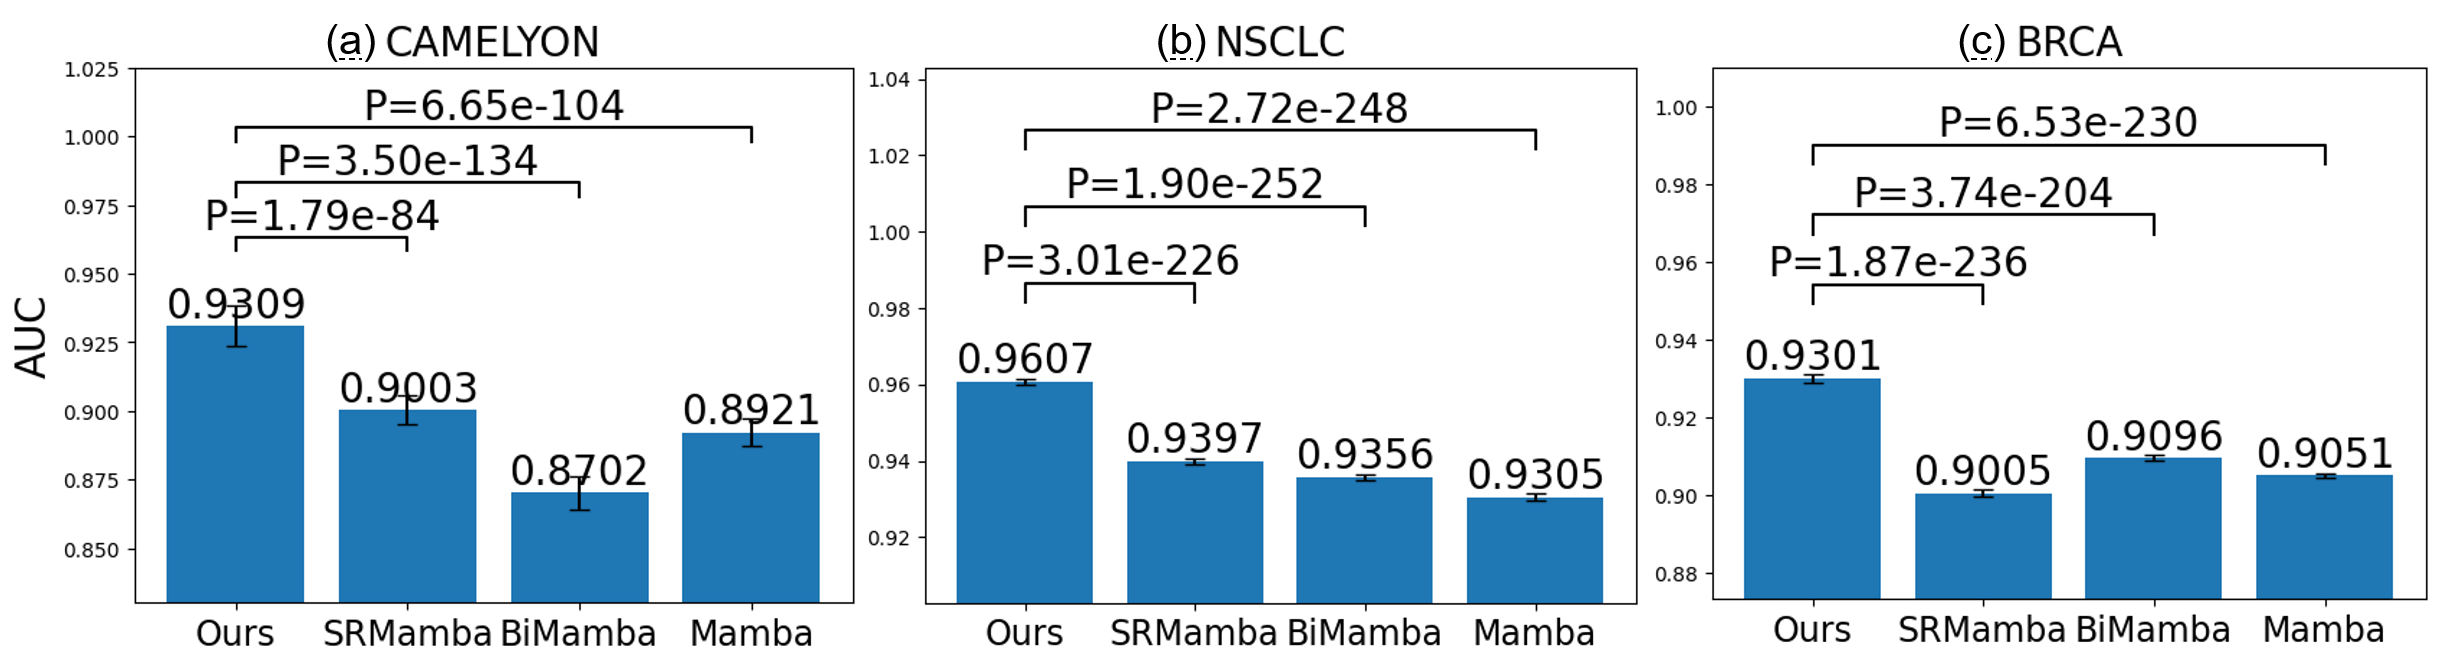
\includegraphics[width=1.0\columnwidth]{figures/scan_invariant.png}
  \bicaption[不同Mamba变体的扫描不变性评估的双样本t检验]{不同Mamba变体的扫描不变性评估的双样本t检验}[Two-sample t-test for scanning invariance evaluation of different Mamba variants]{Two-sample t-test for scanning invariance evaluation of different Mamba variants.}
  \label{figure4: scan-invariant}
  % \vspace{-4pt}
\end{figure}

为了验证本章的方法使Mamba能够构建更多的扫描不变性特征,本章将三个随机选择的扫描序列输入到训练的Mamba变体中进行推理,并分别计算其AUC的平均值和标准差。
实验结果见表\ref{table4: scan-invariant}。与基线相比,本章的方法在CAMELYON和NSCLC数据集上的标准差降低了2倍,在BRACS-7数据集上的标准差降低了3倍。
值得注意的是,本章的方法不仅在所有数据集中实现了最高的平均AUC,而且还显示出最小的标准差,并且与基准实验(表\ref{table4: CAMELYON}、\ref{table4: NSCLC}、\ref{table4: BRCA}和表\ref{table4: BRACS_7})中的正常输入的实验结果相差无几。
这强调了本章的方法在指导Mamba模型学习扫描序列的更多不变特征方面的有效性,优于其他Mamba变体方法。

为了进一步验证本章方法的扫描不变性,本章重复了验证过程,将随机化的数量增加到100,并进行了双样本t检验,如图~\ref{figure4: scan-invariant}所示。结果显示,本章的方法不仅在平均值方面优于其他Mamba方法,而且p值远低于0.05。这表明,在统计意义上,其他Mamba方法与本章方法具有显著的差异。

\textbf{(3)不同Mamba模型性能比对}

\begin{figure}[h!]
  \centering
  \captionsetup{font={small, stretch=1.312}}
  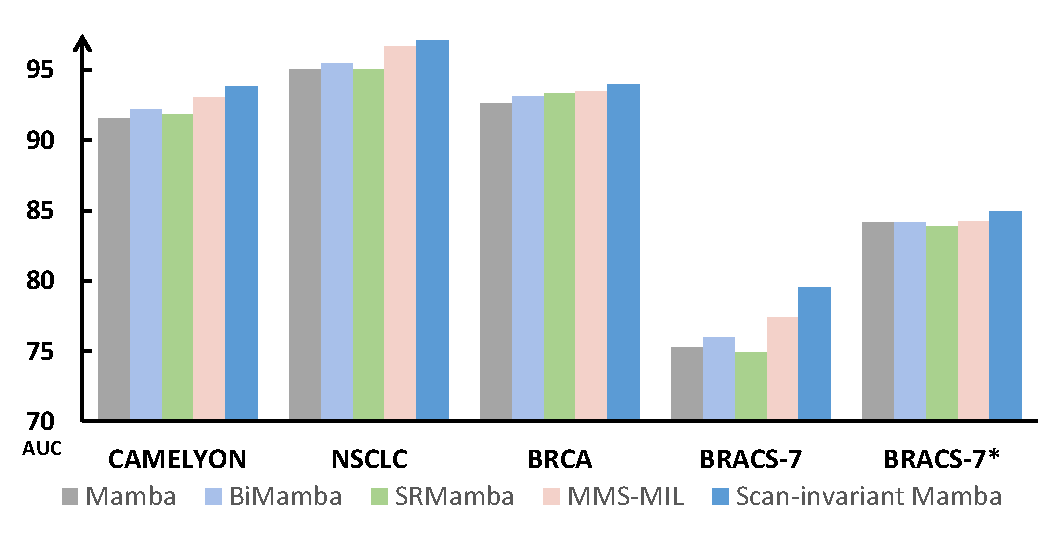
\includegraphics[width=0.9\columnwidth]{figures/SMCMIL的不同Mamba比较.pdf}
  \bicaption[不同Mamba模型性能比对柱状图]{不同Mamba模型性能比对柱状图。}[Bar chart of performance comparison of different Mamba models.]{Bar chart of performance comparison of different Mamba models.}
  \label{figure4: DifferentMamba}
  % \vspace{-4pt}
\end{figure}

为了进一步验证本章的方法的优越性来源于本章的架构而不是Mamba本身,本章对三种变体进行了比较实验:图\ref{figure4: DifferentMamba}中的Mamba Block、BiMamba和SRMamba。
结果表明,SMC-MIL在所有四个数据集上的所有六个任务中都取得了最佳性能。
本章的方法不仅在性能上超过了原始的单分支Mamba,而且在多序列(或扫描)聚合方法(例如,BiMamba和SRMamba,以及上一章提出的方法)中表现出许多优势。
实验结果表明,扫描不变Mamba算法比多扫描集成Mamba算法具有更强的实例建模能力,能够提取更多的判别性特征。


\textbf{(4)不同的分支对比策略对模型性能的影响}

\begin{table}[h!]
  \large    % 设置表格字体为5号
  \setstretch{1.245}        % 设置具有指定弹力的橡皮长度(原行宽的1.2倍)
  \captionsetup{font={small, stretch=1.512}}
  \centering
  % \vspace{-10pt}
  \bicaption[不同的分支对比策略对模型性能的影响]{不同的分支对比策略对模型性能的影响。最优结果用粗体表示,次优结果用下划线表示。}{Effects of different branch contrast strategies on model performance. The best results are shown in bold.}    % 中英文标题
  \begin{tabularx}{\textwidth}{lCCCC}
    \toprule
    方法 & CAMELYON& NSCLC& BRACS-3& BRACS-7\\ \midrule
  vanilla vs. hard & \underline{93.13$\pm$1.90} & 96.30$\pm$1.23 & 84.89$\pm$0.73 & \underline{76.52$\pm$0.32}\\
  easy vs. vanilla & 92.64$\pm$1.33 & \underline{96.55$\pm$1.21} & 82.66$\pm$4.39 & 77.44$\pm$0.95 \\
  hard vs. hard  &  90.39$\pm$2.55 & 95.79$\pm$1.48 & 82.57$\pm$1.83 & 77.22$\pm$2.65 \\
  easy vs. easy & 91.66$\pm$2.10 & 96.35$\pm$1.23  & \underline{85.63$\pm$0.84} & 74.48$\pm$1.61 \\ 
  \textbf{easy vs. hard} & \textbf{93.81$\pm$1.65} & \textbf{96.65$\pm$1.46} & \textbf{87.74$\pm$0.36} & \textbf{79.57$\pm$0.42} \\
    \bottomrule
  \end{tabularx}
  % \vspace{-25pt}
  \label{table4: Different branch}
\end{table}

表\ref{table4: Different branch}列出了五种不同分支对比策略下SMC-MIL的性能。结果表明,“easy vs hard”策略产生最佳性能。
表现如此优异的主要原因是“Easy”分支帮助Mamba产生可靠的包表示和分类,而“hard”分支迫使模型不仅要学习扫描无关的特征,还要从被屏蔽序列中探索更多的判别实例,以实现两个分支之间的一致性。
此外,两个分支的差异也有利于性能提升。“hard vs hard”策略表现最差。本章将其性能较差归因于在包表示和分类中缺乏来自“Easy”分支的可靠指导。

\textbf{(5)讨论不同扫描模式的组合对模型性能的影响}

\begin{table}[h!]
  \large    % 设置表格字体为5号
  \setstretch{1.245}        % 设置具有指定弹力的橡皮长度(原行宽的1.2倍)
  \captionsetup{font={small, stretch=1.512}}
  \centering
  % \vspace{-10pt}
  \bicaption[讨论不同扫描模式的组合对模型性能的影响]{讨论不同扫描模式的组合对模型性能的影响。最优结果用粗体表示。}{Effect of combinations of different scan patterns on model performance. The best results are shown in bold.}    % 中英文标题
  \begin{tabularx}{\textwidth}{lCCCC}
    \toprule
    方法 & CAMELYON& NSCLC& BRCA& BRACS-7$^\star$\\ \midrule
    Origin vs. Backward & {92.64$\pm$1.36} & \textbf{96.65$\pm$1.46} & \textbf{93.98$\pm$1.02} & \textbf{85.11$\pm$2.14} \\
    Origin vs. Random & \textbf{93.81$\pm$1.65} & {96.40$\pm$1.09} & {93.20$\pm$1.50} & {84.75$\pm$2.79} \\
    Origin vs. Grid. &  92.70$\pm$2.80 & 96.32$\pm$1.78 & 93.62$\pm$1.65 & 84.59$\pm$1.33 \\
    Origin vs. RSS. &  92.26$\pm$2.17 & 95.78$\pm$1.28 & 93.73$\pm$1.98 & 84.48$\pm$2.00 \\
    Random vs. Random  &  92.10$\pm$2.20 & 95.79$\pm$1.08 & 92.87$\pm$1.02 & 83.45$\pm$1.74 \\
    \bottomrule
  \end{tabularx}
  % \vspace{-25pt}
  \label{table4: Different scan}
\end{table}

比较不同的扫描模式可能会产生不同的结果。因此,本章还研究了使用不同形式的对比对SMC-MIL性能的影响。
如表\ref{table4: Different scan}所示,在CAMELYON数据集上,通过比较原始扫描模式和随机扫描模式可以获得最佳性能,而在其他数据集上,原始扫描模式和反向扫描模式可以获得最佳效果。
因此,在CAMELYON实验中,本章使用原始扫描模式和随机扫描模式来生成不同顺序的序列,对于剩余的数据集,本章使用原始扫描模式和反向扫描模式。
本小节同样对比了上一章提出的网格扫描和区域螺旋扫描模式,同样取得不错的性能。这侧面说明第三章提出的扫描模式补足了原始序列没有的空间信息。

\textbf{(6)讨论序列增强率的影响\texorpdfstring{$\alpha\%$}{}}

\begin{figure}[h!]
  \centering
  \captionsetup{font={small, stretch=1.312}}
  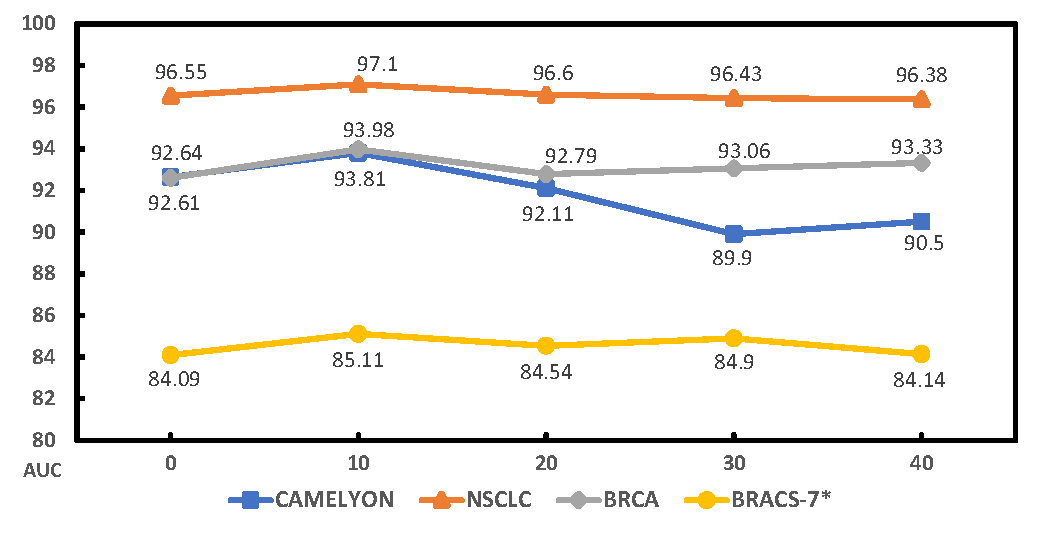
\includegraphics[width=0.8\columnwidth]{figures/MixRatio.pdf}
  \bicaption[不同序列增强率\texorpdfstring{$\alpha\%$}{}下的模型性能折线图]{不同序列增强率\texorpdfstring{$\alpha\%$}{}下的模型性能折线图。}[Line plot of model performance for different sequence enhancement rates \texorpdfstring{$\alpha\%$}{}]{Line plot of model performance for different sequence enhancement rates \texorpdfstring{$\alpha\%$}{}.}
  \label{figure4: mixratio}
\end{figure}

图~\ref{figure4: mixratio}讨论了超参数序列增强率$\alpha\%$的影响。为了更好地突出实验结果,本章将BRACS-7$^\star$结果绘制在副轴上。
如图所示,除CAMELYON外,大多数数据集在序列增强率为0.1时达到最佳性能,CAMELYON在$\alpha\%=40\%$时达到峰值。为了保持一致性,本章将所有数据集的序列扩增率$\alpha\%$默认设置为$10\%$。


\textbf{(7)讨论序列掩码率的影响\texorpdfstring{$\beta\%$}{}}

\begin{figure}[h!]
  \centering
  \captionsetup{font={small, stretch=1.312}}
  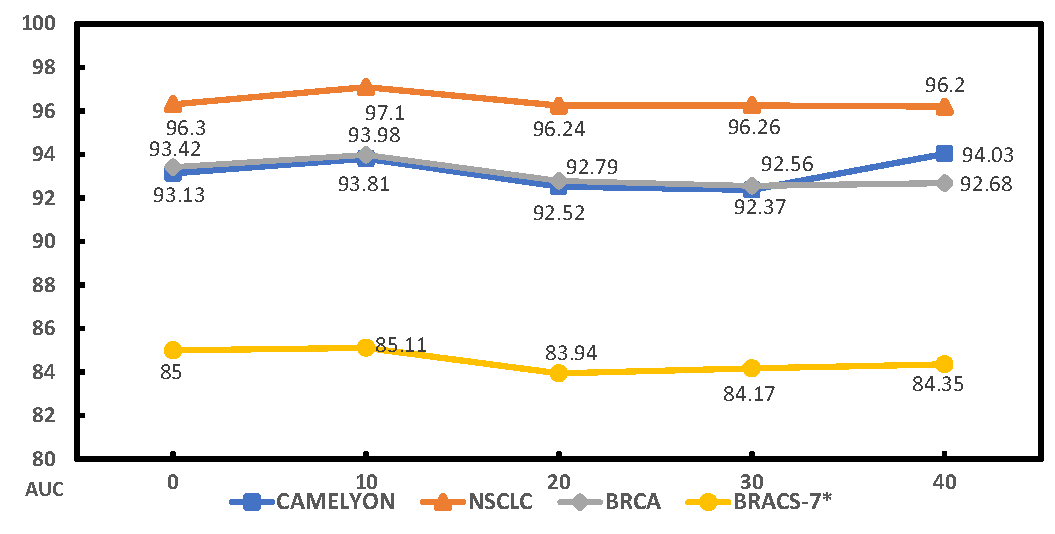
\includegraphics[width=0.8\columnwidth]{figures/MaskRatio.pdf}
  \bicaption[不同序列掩码率\texorpdfstring{$\beta\%$}{}下的模型性能折线图]{不同序列掩码率\texorpdfstring{$\beta\%$}{}下的模型性能折线图。}[Line plot of model performance for different sequence masking ratess \texorpdfstring{$\beta\%$}{}]{Line plot of model performance for different sequence masking ratess \texorpdfstring{$\beta\%$}{}.}
  \label{figure4: maskratio}
\end{figure}

图~\ref{figure4: maskratio}讨论了超参数序列掩码率$\beta\%$的影响。本小节与前一小节一致,同样在次级轴上绘制了BRACS-7$^\star$结果。
所有数据集在$10\%$的序列掩码率下达到最佳性能。因此,除非另有说明,否则本章默认设置$\beta\% = 10\%$。

\textbf{(8)Bootstrap检验}

\begin{figure}[h!]
  \centering
  \captionsetup{font={small, stretch=1.312}}
  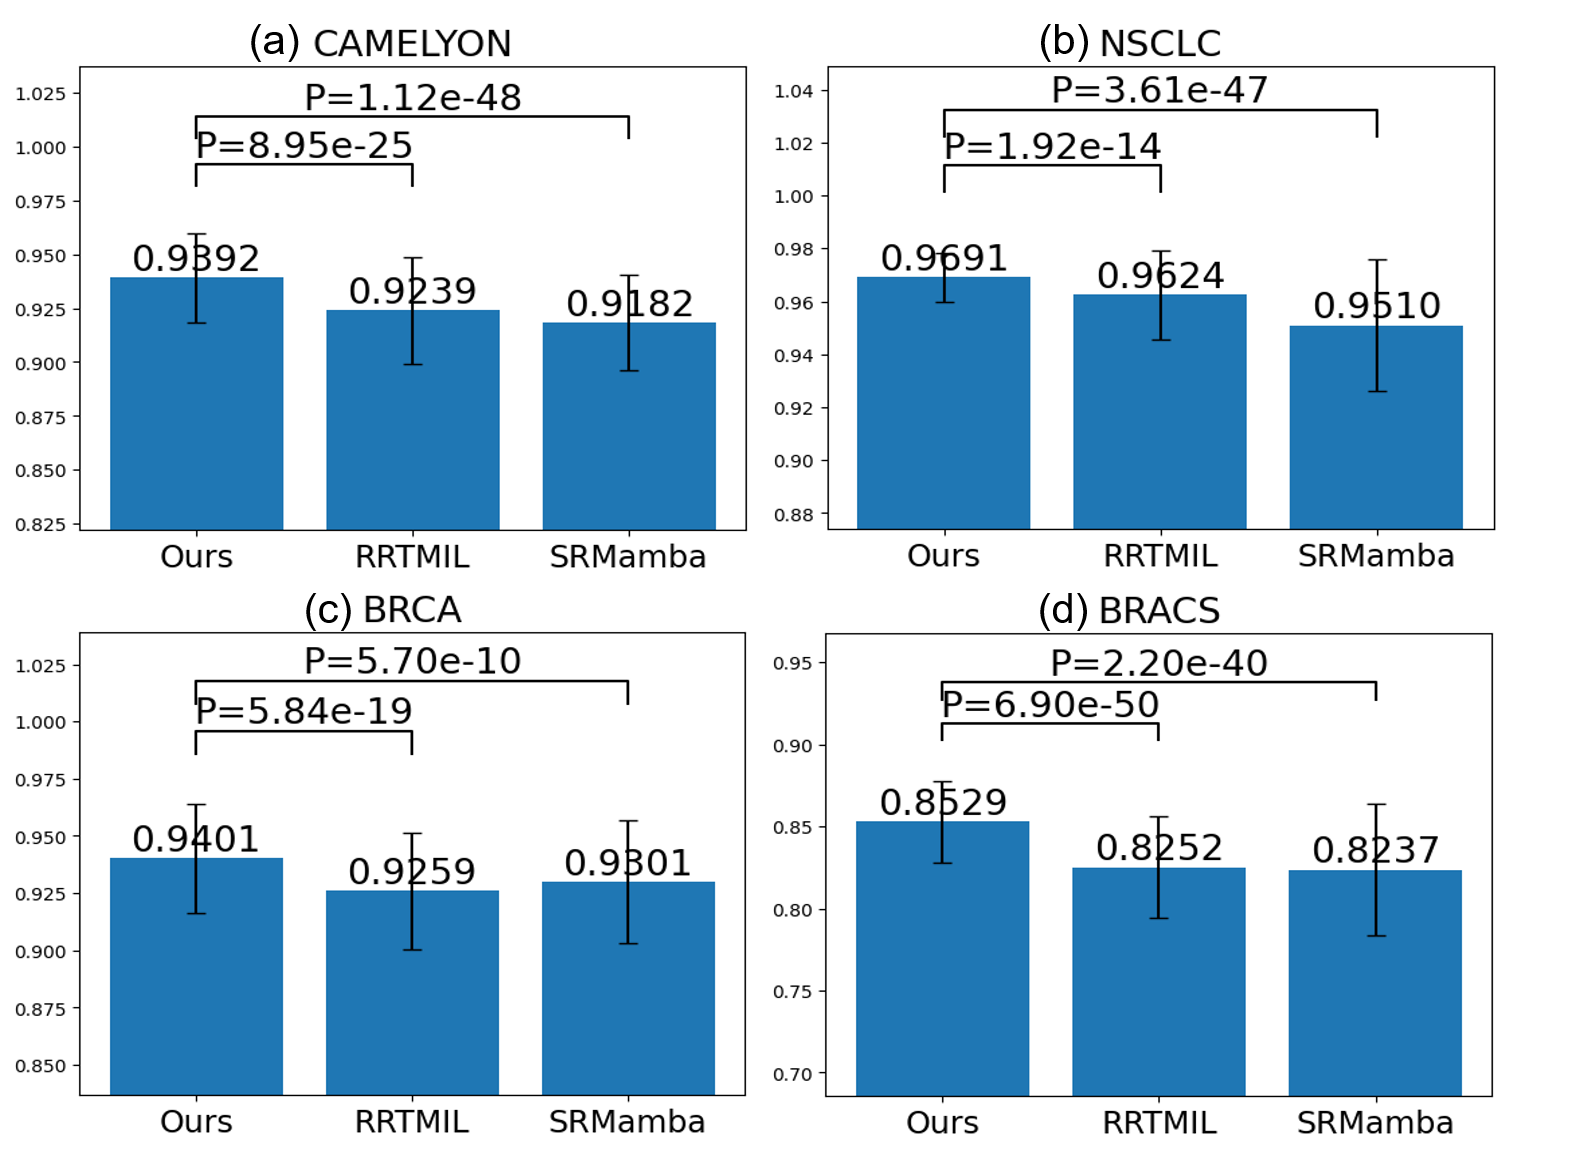
\includegraphics[width=0.8\columnwidth]{figures/t-testwithSOTA.png}
  \bicaption[与SOTA方法性能比较的Bootstrap检验]{与SOTA方法性能比较的Bootstrap检验。}[Bootstrap test for performance comparison with SOTA method]{Bootstrap test for performance comparison with SOTA method.}
  \label{figure4: sota t-test}
\end{figure}
本小节对本章方法和SOTA方法进行了有放回的随机抽样Bootstrap检验,共采样100次,得到的结果如图~\ref{figure4: sota t-test}所示。可以看出,本章的方法显著高于SOTA,因为p值远小于0.05。

\textbf{(9)两种推理方式的性能对比}

\begin{table}[h!]
  \large    % 设置表格字体为5号
  \setstretch{1.245}        % 设置具有指定弹力的橡皮长度(原行宽的1.2倍)
  \captionsetup{font={small, stretch=1.512}}
  \centering
  % \vspace{-10pt}
  \bicaption[不同推理方式的性能对比]{不同的推理方式的性能对比。最优结果用粗体表示。}{Performance comparison of different inference modes. The best results are shown in bold.}    % 中英文标题
  \begin{tabularx}{\textwidth}{lCCCC}
    \toprule
    方法 & CAMELYON& NSCLC& BRACS-3& BRACS-7\\ \midrule
    w/ 序列增强模块 & \textbf{93.81$\pm$1.65} & 96.65$\pm$1.46 & \textbf{87.74$\pm$0.36} & \textbf{79.57$\pm$0.42} \\
    w/o 序列增强模块  & 93.70$\pm$1.42 & \textbf{96.67$\pm$1.31} & 87.65$\pm$4.17 & 79.43$\pm$0.95 \\
    \bottomrule
  \end{tabularx}
  % \vspace{-25pt}
  \label{table4: Different inference}
\end{table}
本小节讨论了使用不同推理方式对性能结果的影响,结果报告在表~\ref{table4: Different inference}中。
可以看出两者并没有明显的差异,这更证明本章所提出模型的泛化性能。
默认设置下,本文采用有序列增强模块的推理模式进行推理。

\begin{table}[h!]
  \large    % 设置表格字体为5号
  \setstretch{1.245}        % 设置具有指定弹力的橡皮长度(原行宽的1.2倍)
  \captionsetup{font={small, stretch=1.512}}
  \centering
  % \vspace{-10pt}
  \bicaption[SMC-MIL以PLIP为离线特征提取器的癌症诊断性能]{SMC-MIL以PLIP为离线特征提取器的癌症诊断性能。最优结果用粗体表示,次优结果用下划线表示。}{Cancer diagnosis performance of SMC-MIL with PLIP as the offline feature extractors. The optimal experimental results are marked in bold, and the sub-optimal are underlined.}    % 中英文标题
  \begin{tabularx}{\textwidth}{clCCC}
    \toprule
    &方法  & Accuracy& AUC&F1-score\\ \midrule
    \multirow{6}{*}{\rotatebox{90}{PLIP}}&AB-MIL  & 90.09$\pm$1.63 & \underline{94.55$\pm$1.91} & 86.48$\pm$2.50\\
    &OriginMamba        & 90.87$\pm$1.52 & 94.44$\pm$2.19 & 87.78$\pm$1.89\\
    &BiMamba          & 90.54$\pm$1.89 & 94.20$\pm$1.99 & 86.82$\pm$2.77\\
    &SRMamba & \underline{91.87$\pm$0.85} & 94.20$\pm$2.16 & \underline{88.37$\pm$1.31}\\
    &%\textbf{M$^2$S-MIL}
    第三章方法 & \underline{92.21$\pm$0.60} & \underline{95.24$\pm$1.85} & \underline{89.46$\pm$0.93}\\  
    &\textbf{SMC-MIL}        & \textbf{92.50$\pm$0.87} & \textbf{95.79$\pm$1.31} & \textbf{89.99$\pm$0.43}\\  
    \bottomrule
  \end{tabularx}
 \vspace{-25pt}
  \label{table4: CAMELYON_PLIP}
\end{table}
\begin{table}[h!]
  \large    % 设置表格字体为5号
  \setstretch{1.245}        % 设置具有指定弹力的橡皮长度(原行宽的1.2倍)
  \captionsetup{font={small, stretch=1.512}}
  \centering
  % \vspace{-10pt}
  \bicaption[SMC-MIL以PLIP为离线特征提取器在TCGA-NSCLC上的亚型分型性能]{SMC-MIL以PLIP为离线特征提取器在TCGA-NSCLC上的的亚型分型性能。最优结果用粗体表示,次优结果用下划线表示。}{Cancer sub-typing performance of SMC-MIL on the TCGA-NSCLC dataset with PLIP as the feature extractors. The optimal experimental results are marked in bold, and the sub-optimal experimental results are underlined.}    % 中英文标题
  \begin{tabularx}{\textwidth}{clCCC}
    \toprule
    &方法  & Accuracy& AUC&F1-score\\ \midrule
    \multirow{6}{*}{\rotatebox{90}{PLIP}}&AB-MIL  & 89.94$\pm$1.84 & 94.45$\pm$1.64 & 89.43$\pm$1.97\\
    &OriginMamba        & 90.89$\pm$1.60 & 95.57$\pm$1.60 & 90.24$\pm$1.84\\
    &BiMamba          & 90.70$\pm$1.95 & 95.42$\pm$1.68 & 89.94$\pm$2.26\\
    &SRMamba &  89.85$\pm$2.07 & 95.72$\pm$1.51 & 88.96$\pm$2.66 \\
    &%\textbf{M$^2$S-MIL}
    第三章方法  & \underline{91.56$\pm$1.76} & \underline{96.22$\pm$1.12} & \underline{90.64$\pm$1.86}\\     
    &\textbf{SMC-MIL}        & \textbf{92.30$\pm$0.60} & \textbf{96.78$\pm$1.68} & \textbf{91.79$\pm$0.50}\\  

    \bottomrule
\end{tabularx}
\vspace{-25pt}

  \label{table4: NSCLC_PLIP}
\end{table}

\begin{table}[h!]
  \large    % 设置表格字体为5号
  \setstretch{1.245}        % 设置具有指定弹力的橡皮长度(原行宽的1.2倍)
  \captionsetup{font={small, stretch=1.512}}
  \centering
  % \vspace{-10pt}
  \bicaption[SMC-MIL以PLIP为离线特征提取器在TCGA-BRCA上的亚型分型性能]{SMC-MIL以PLIP为离线特征提取器在TCGA-BRCA上的亚型分型性能。最优结果用粗体表示,次优结果用下划线表示。}{Cancer sub-typing performance of SMC-MIL on the TCGA-BRCA dataset with PLIP as the feature extractors. The optimal experimental results are marked in bold, and the sub-optimal experimental results are underlined.}    % 中英文标题
  \begin{tabularx}{\textwidth}{clCCC}
    \toprule
    &方法  & Accuracy& AUC&F1-score\\ \midrule
    
    \multirow{6}{*}{\rotatebox{90}{PLIP}}&AB-MIL  & 83.81$\pm$3.72 & 90.18$\pm$2.99 & 67.94$\pm$4.22\\
  &OriginMamba        & 86.75$\pm$5.76 & 92.90$\pm$2.44 & 74.35$\pm$7.23\\
  &BiMamba          & 87.73$\pm$3.06 & 92.64$\pm$2.28 & 74.07$\pm$4.75\\
  &SRMamba & 86.40$\pm$3.31 & 92.17$\pm$2.67 & 72.39$\pm$4.62\\
  &%\textbf{M$^2$S-MIL} 
  第三章方法   & \underline{88.82$\pm$3.22} & \underline{93.40$\pm$1.24} & \underline{75.00$\pm$2.50}\\  
  &\textbf{SMC-MIL}        & \textbf{89.75$\pm$0.54} & \textbf{94.71$\pm$1.49} & \textbf{75.37$\pm$0.98}\\  

  \bottomrule
\end{tabularx}

  \label{table4: BRCA_PLIP}
\end{table}

\textbf{(10)使用PLIP作为特征提取器的性能结果}





\begin{figure}[h!]
  \centering
  \captionsetup{font={small, stretch=1.312}}
  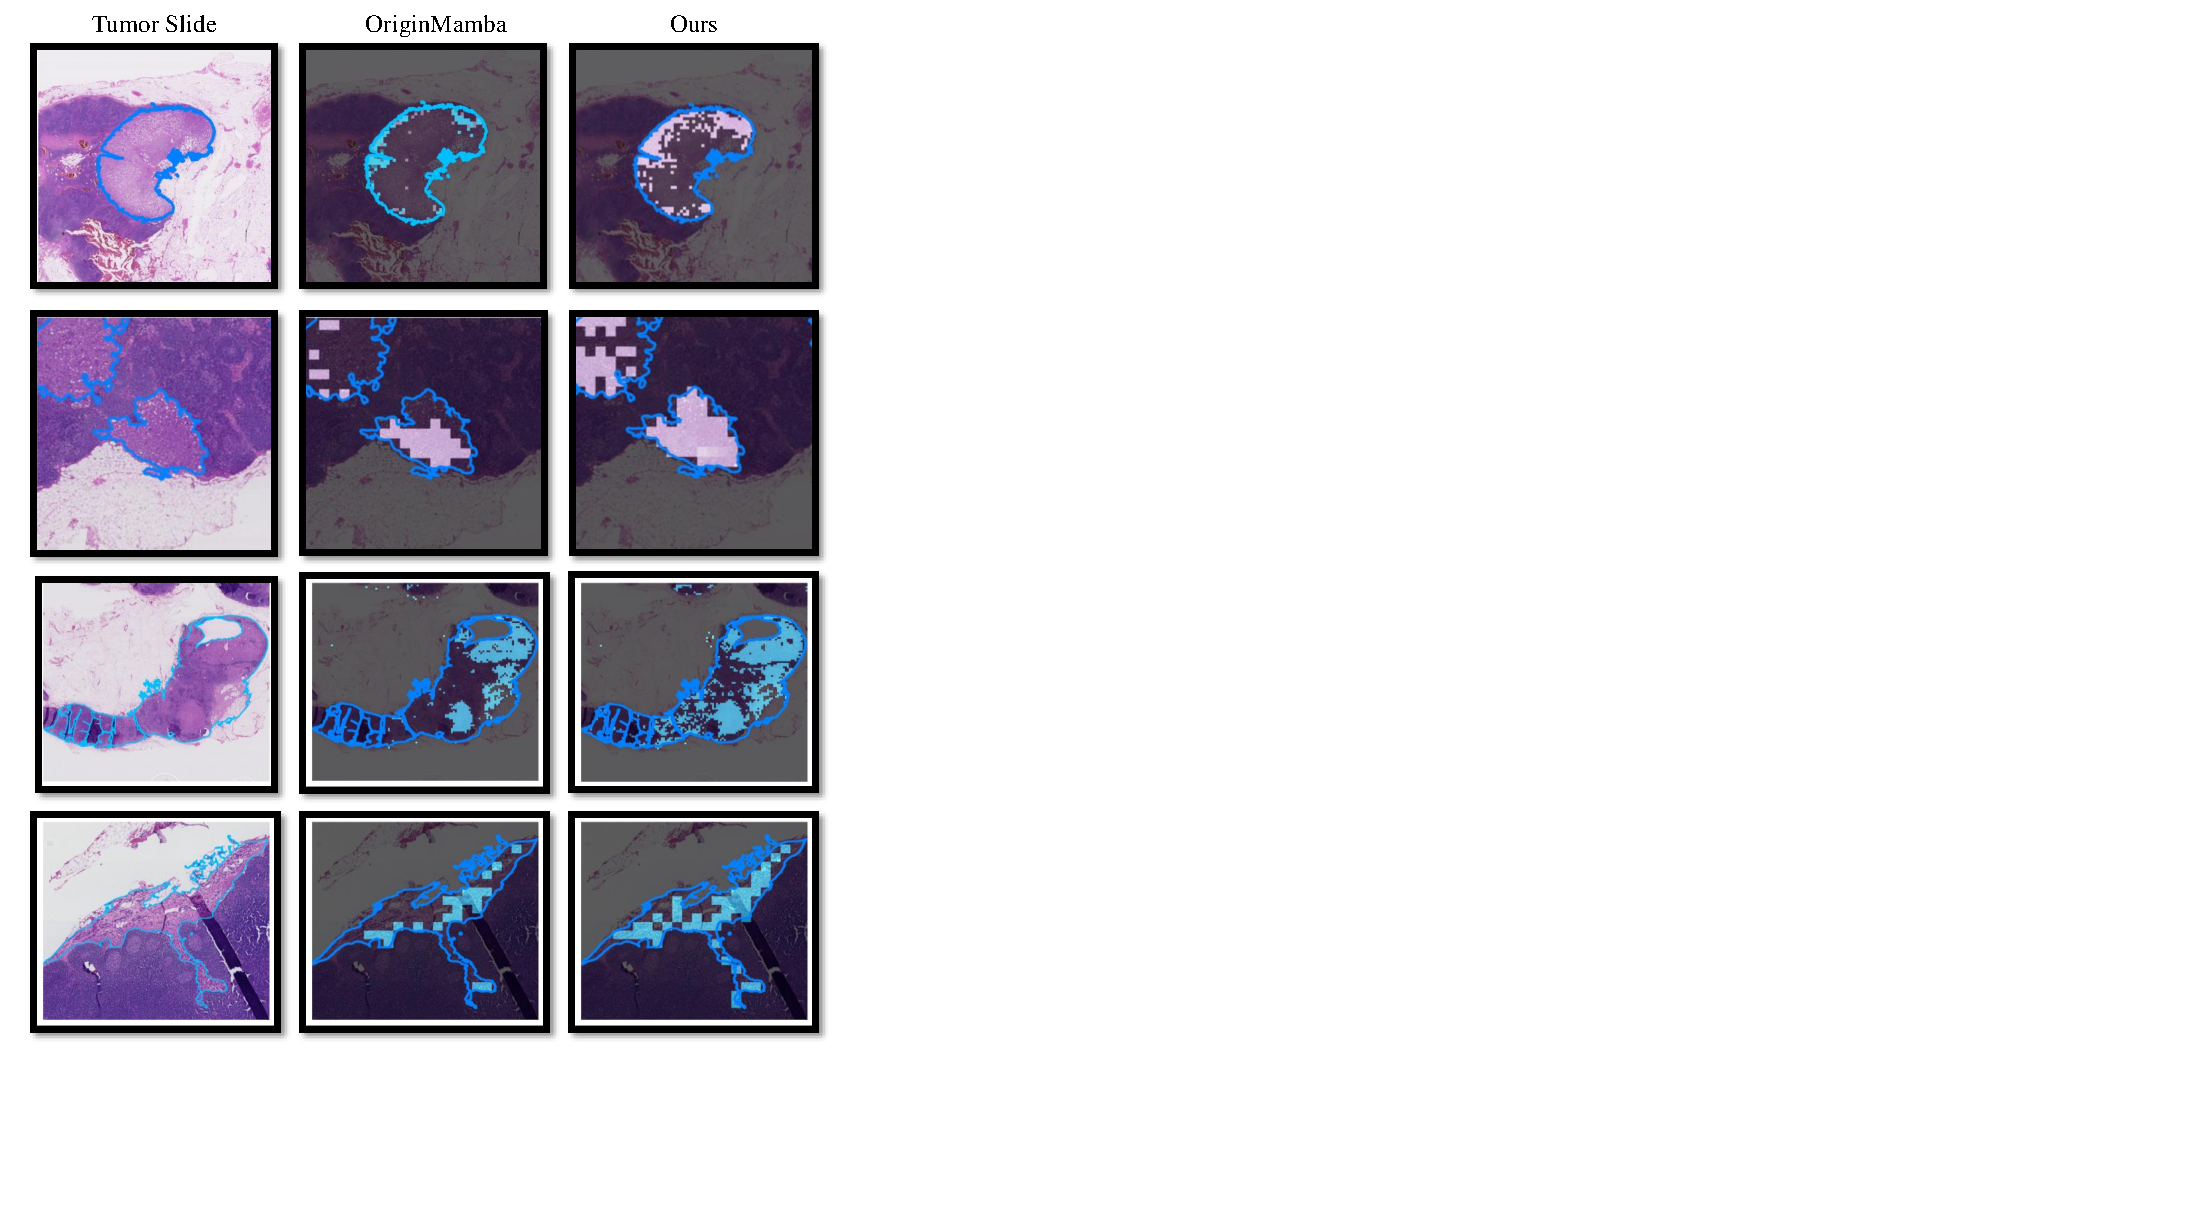
\includegraphics[width=0.8\columnwidth]{figures/Visualize_cropped.pdf}
  \bicaption[原始Mamba(baseline)和SMC-MIL关注的图块可视化结果]{原始Mamba(baseline)和SMC-MIL制作的图块可视化结果}[Visualization results of patches focused by original Mamba(baseline) and SMC-MIL]{Visualization results of patches focused by original Mamba(baseline) and SMC-MIL.}
  \label{figure4: visualize}
\end{figure}

\begin{figure}[h!]
  \centering
  \captionsetup{font={small, stretch=1.312}}
  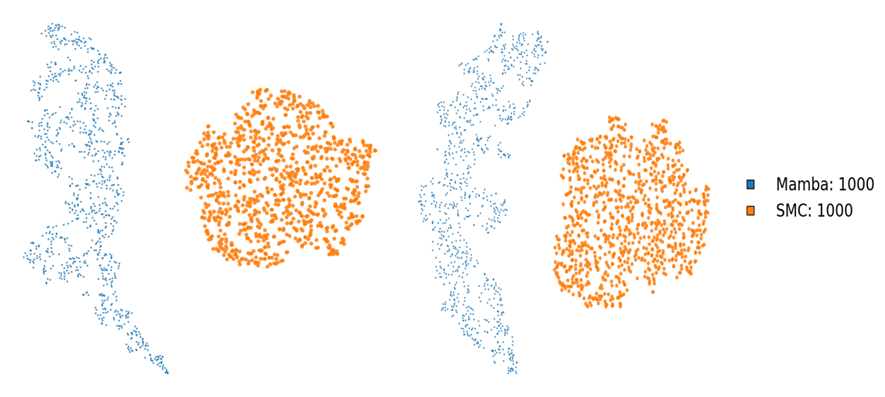
\includegraphics[width=0.8\columnwidth]{figures/t-SNE.png}
  \bicaption[原始Mamba(baseline)和SMC-MIL聚合特征t-SNE可视化结果]{原始Mamba(baseline)和SMC-MIL聚合特征t-SNE可视化结果}[The t-SNE visualization of aggregated features from original Mamba(baseline) and SMC-MIL]{The t-SNE visualization of aggregated features from Mamba(baseline) and SMC-MIL.}
  \label{figure4: tSNE}
\end{figure}


为了进一步探索本章方法的有效性,本小节还进行了将同样采用自监督预训练的PLIP~\cite{huang2023visual}作为特征提取器的相关实验,以验证本章方法的普遍适用性。
如表\ref{table4: CAMELYON_PLIP}、\ref{table4: NSCLC_PLIP}和\ref{table4: BRCA_PLIP}所示,可以看出实验结果与R50特征一致。
本章的方法优于其它基于Mamba的方法。在CAMELYON数据集上,它在精度、AUC和F1-score方面分别比次优的方法提高了0.29\%、0.55\%和0.53\%。这些指标在NSCLC数据集中分别为0.74\%,0.36\%和1.15\%。
最后,BRCA数据集的改进也值得注意,Acc提高了0.93\%,AUC提高了1.31\%,F1-score提高了0.37\%。
这进一步表明,即使使用非传统的ResNet-50特征提取器,本章方法的性能改进也不仅仅是依赖于简单的多个Mamba分支合并,而是正确捕获了空间信息与视觉特征。



\subsection[\hspace{-2pt}可视化分析]{{\heiti\zihao{4} \hspace{-8pt}可视化分析}}\label{section4: 可视化分析}






为了直观地验证本章方法的可解释性,本章将OriginMamba和本章的方法在Camelyon-16数据集上产生的高注意力分数的实例可视化,如图\ref{figure4: visualize}所示。蓝色的线条勾勒出肿瘤区域。越亮的斑块表明注意力得分越高。可视化结果清楚地表明,与原始Mamba相比,SMC-MIL能够更准确地选择显著斑块。
 
并且为了更加充分验证本章方法的扫描不变性,本章用t-SNE可视化了同一个WSI切片经过N个不同扫描模式所建模出的N个包特征,结果展示在图\ref{figure4: tSNE}(展示图中N为1000)。
可以看到SMC-MIL建模出的包特征明显更为集中,而原始Mamba的建模更为分散。实验充分说明本章所提出的基于序列差异化对比的Mamba模型具有扫描不变性。

\section[\hspace{-2pt}本章小结]{{\heiti\zihao{-3} \hspace{-8pt}本章小结}}\label{section4: 本章小结}

本章针对原始Mamba倾向性建模出因果关系与病理图像多实例学习的序列不变性存在冲突的问题,以引导Mamba建模与顺序无关的包特征为切入点,
提出了一种基于Mamba和对比学习的MIL框架,以解决扫描敏感Mamba和扫描不变MIL之间的差距。
该框架通过对不同扫描分支的结果应用一致性约束,指导Mamba从不同序列中学习包的扫描不变特征。
此外,序列对比度增强分别用于增强和掩码序列,迫使Mamba识别更多的鉴别斑块。
在3个WSI子任务以及12个基准上的大量对比及消融实验表明,该框架优于最新的其他方法,并且本章的方法解决了多扫描信息整合的策略存在无法穷举所有扫描情况,高度依赖扫描模式和集成方式的问题,有效地减轻了Mamba在MIL任务中的局限性,
使其更适合这些任务,并为Mamba在视觉任务中的进一步应用铺平了道路。
%未来,作者将致力于探索扫描不变性Mamba在更困难病理图像任务上的可能,如定位和分割。
\chapter[\hspace{0pt}总结与未来展望]{{\heiti\zihao{3}\hspace{0pt}总结与未来展望}}\label{section 7}
\removelofgap
\removelotgap

本章内容共分为两节,\hyperref[section5: 总结]{第一节}对本文研究内容与方法进行总结;\hyperref[section5: 未来展望]{第二节}会阐述本文提出方法存在的局限之处,同时对后续的研究方向展开展望。


\section[\hspace{-2pt}总结]{{\heiti\zihao{-3} \hspace{-8pt}总结}}\label{section5: 总结}


本研究聚焦于 Mamba 架构在病理图像分类领域的应用,旨在解决该架构在面对病理图像分类任务时所暴露出的一系列问题。
病理图像分类任务由于实例数目众多,常导致计算资源消耗巨大,同时实例间关系建模也往往不够充分。
Mamba 架构虽在一定程度上有效应对了这些挑战,
但其仍存在无法充分捕获二维空间关系,以及与病理图像多实例学习的序列不变性存在冲突的问题。​

为解决上述问题,实现 Mamba 架构在病理图像领域的高效适配,
本研究从多扫描模式融合 Mamba 和扫描不变性 Mamba 两个独特角度展开深入研究:

(1)在基于多扫描 Mamba 的高分辨率病理图像分类研究方面,
鉴于Mamba一维序列建模所造成图像空间结构捕获能力不足的问题,研究提出了基于空间信息增强实现的多扫描 Mamba 的多实例学习框架。
该框架创新性地设计了多个扫描模式分支作为Mamba的输入,提出了区域螺旋扫描和网格扫描等新型扫描模式,显著提升了 Mamba 对局部连续性、旋转不变性以及同一序列不同方向空间关联信息的捕获能力。
同时,通过设计基于分块局部注意力的2D空间上下文感知模块,进一步强化序列对2D空间上下文的感知能力,
通过区域内信息整合,极大地提高了Mamba对空间能力的捕捉,
有力地推动了Mamba模型与病理图像分类任务的适配进程。
在3个WSI分析子任务和7个数据集上进行的大量实验充分证明,综合多种扫描模式分支并引入空间信息,
能够切实解决Mamba从一维实例序列中空间建模不充分的问题,显著提高模型性能,同时起到一定缓解数字病理图像分类任务中使用Mamba模型时出现的建模倾向差异的作用。​

(2)在基于扫描不变性Mamba的高分辨率病理图像分类研究方面,
%利用多扫描模式信息融合缓解Mamba建模能力与病理图像任务间差异的思路固然直接,
%但其仅是一种妥协的方案,高度依赖扫描模式和集成形式。
%基于此,
针对Mamba作为序列相关模型,与病理图像多实例学习的序列不变性存在冲突的问题,研究提出了基于对比学习策略的扫描不变 Mamba 的多实例学习框架。
为引导 Mamba 学习到不同实例扫描序列中一致的包特征,精心设计了双分支实例序列对比学习框架,强制在两个极端不同的扫描序列之间,通过相同的 Mamba 获得的包表示及分类 logits 值保持一致性。
同时,还设计了一种基于实例评估的序列对比增强方法,不仅增加了对比学习的难度,还迫使 Mamba 在输入序列差异极大的情况下,学习对 WSI 图像形成一致的表示和决策,成功赋予了 Mamba 良好的序列不变建模和判别实例识别能力。
同样在3个WSI分析子任务和12个基准上开展的广泛系统实验结果显示,SMC-MIL 能够在让 Mamba 继承其优异计算效率和建模能力的同时,有效降低模型对输入序列顺序的敏感性,专注于实例无序关系建模,挖掘出更具显著性判别的特征,从而更好地适配病理图像分类任务。​

总体而言,本研究提出的M$^2$S-MIL模型和SMC-MIL模型,分别从多扫描模式Mamba和扫描不变性Mamba两个维度,对数字病理图像分类任务中Mamba的应用进行了全面且深入的剖析与研究。
M$^2$S-MIL 模型通过综合多种扫描模式的特征信息,并引入空间上下文感知模块,显著提升了 Mamba 对 2D 空间信息的捕获能力,有效缓解了原本Mamba一维序列建模所造成图像空间结构捕获能力不足的问题;
SMC-MIL 模型则进一步突破了扫描顺序对 Mamba 建模能力的束缚,成功弥合了原本 Mamba 的序列敏感性与病理图像多实例学习中序列不变性假设之间的冲突,使 Mamba 架构更加契合病理图像任务,同时提高了模型挖掘更具判别性区域的能力,进而提升了模型性能。​


\section[\hspace{-2pt}未来展望]{{\heiti\zihao{-3} \hspace{-8pt}未来展望}}\label{section5: 未来展望}

本文分析了在 Mamba 架构适配病理图像分类任务方面的挑战,以数据的视觉特征和任务特点为切入点,从多扫描信息融合和构造扫描不变性Mamba两个角度入手,提出了基于空间信息增强的多扫描Mamba模型和基于差异化序列对比的扫描不变Mamba模型来解决高分辨率病理图像分类问题,取得了一定成果,但仍存在诸多可拓展与深入研究的方向。​

在扫描优化层面,未来可进一步探索更高效的扫描模式设计。现有的区域螺旋扫描和网格扫描虽已取得良好效果,但随着病理图像复杂性的不断增加,可能需要研发更具针对性、能够更精准捕捉图像特征的扫描模式。例如,可以结合病理图像中不同组织类型、病变特征的分布特点,设计自适应的扫描模式,使 Mamba 能够更快速、准确地获取关键信息。​

对于对比学习策略,也有很大的提升空间。当前的双分支实例序列对比学习框架和基于实例评估的序列对比增强方法已发挥重要作用,但可以尝试引入更复杂的对比学习算法,如结合生成对抗网络(GAN)的思想,让 Mamba 在与生成器的对抗过程中,学习到更具鲁棒性和判别性的特征表示。同时,在对比学习的过程中,如何更好地平衡模型的训练效率和性能提升,也是需要深入研究的问题。​

从应用拓展角度来看,本文的研究依旧聚焦于多实例学习范式中将离线的特征进行特征聚合。未来可以迁移至特征提取,或者尝试打破范式,探索在线特征提取与实例聚合的病理图像分类方法。

此外,与临床实践的结合也是未来研究的重要方向。目前的研究更多停留在实验室环境下的模型性能验证,而将这些模型真正应用到临床诊断中,还需要解决一系列实际问题,如模型的可解释性、与现有临床诊断流程的兼容性等。通过与临床医生合作,深入了解临床需求,能够使模型的改进更贴合实际应用,为病理诊断提供更有力的支持。​

在数据层面,随着医疗数据的不断积累,如何更好地利用大规模病理图像数据训练 Mamba 模型也是未来研究的重点。一方面,可以探索更有效的数据增强方法,在不改变图像真实病理特征的前提下,增加数据的多样性,提高模型的泛化能力;另一方面,如何从海量数据中筛选出对模型训练最有价值的数据,避免冗余数据对模型性能的影响,也是需要解决的问题。​

最后,随着人工智能技术的不断发展,跨领域技术融合将为病理图像分类带来新的机遇。例如,将 Mamba 架构与知识图谱技术相结合,利用知识图谱中丰富的医学知识,引导 Mamba 更好地理解病理图像中的特征和关系,从而提高分类的准确性和可靠性。总之,未来在 Mamba 架构应用于病理图像分类领域的研究中,仍有广阔的探索空间,有望通过不断的技术创新和应用拓展,为病理诊断领域带来更显著的变革。
%\include{contents/yourFreeChoise}

\backmatter %%% 后置部分(致谢、参考文献、附录等)

%% 参考文献
% 顺序编码制:cqunumerical		
% 注意:至少需要引用一篇参考文献,否则下面两行会引起编译错误。
% \bibliographystyle{cqunumerical}
\bibliographystyle{gbt7714-numerical_new}
\bibliography{ref/refs}


%% 附录(按ABC...分节,证明、推导、程序、个人简历等)
\appendix
\chapter[附\hskip\ccwd{}\hskip\ccwd{}录]{{\heiti\zihao{3}附\hskip\ccwd{}\hskip\ccwd{}录}}

\section[\hspace{-2pt}作者在攻读硕士学位期间的论文目录]{{\heiti\zihao{-3} \hspace{-8pt}作者在攻读硕士学位期间的论文目录}}

%下面是盲审标记\cs{secretize}的用法,记得去\textsf{main.tex}开启盲审开关看效果:

% \circled{1}已发表论文

% \begin{enumerate}
%     \item \textbf{\secretize{XU X}}, \secretize{LIU K}, DAI P, et al. Joint task offloading and resource optimization in NOMA-based vehicular edge computing: A game-theoretic DRL approach[J]. Journal of Systems Architecture, 2023, 134: 102780. 影响因子: 5.836(2021), 4.497(5年) (中科院SCI 2区,对应本文第三章)
% 	\item \textbf{\secretize{许新操}}, \secretize{刘凯}, 刘春晖, 等. 基于势博弈的车载边缘计算信道分配方法[J]. 电子学报, 2021,49(5): 851-860. (EI 索引,CCF T1类中文高质量科技期刊,对应本文第三章)
% 	\item \textbf{ \secretize{XU X}}, \secretize{LIU K}, XIAO K, et al. Vehicular fog computing enabled real-time collision warning via trajectory calibration[J]. Mobile Networks and Applications, 2020, 25(6): 2482-2494. 影响因子: 3.077(2021), 2.92(5年) (中科院SCI 3区,对应本文第五章)
% \end{enumerate}
{
\small
\setlength{\baselineskip}{20pt}
\begin{enumerate}[label={[\arabic*]}, leftmargin=*]
\item Tang W, Zhou F, \secretize{Huang S}, \secretize{\textbf{Zhu X}}, et al. Feature re-embedding: Towards foundation model-level performance in computational pathology[C]//Proceedings of the IEEE/CVF Conference on Computer Vision and Pattern Recognition(CVPR). 2024: 11343-11352. 
\item \secretize{\textbf{Zhu X}}, \secretize{Huang S}, Tang W,  et al. Adaptive Learning of Instance Representatives in Dual Spaces for Medical Image Classification[J]. Neural Computing and Applications (中科院SCI二区,已完成第一次返修)
\item \secretize{\textbf{Zhu X}}, \secretize{Huang S}, Liu B, et al. Scan-invariant Mamba with Contrastive Learning in Computational Pathology[J]. IEEE Transactions on Medical Imaging(SCI一区,Submitted)
\end{enumerate}
}

\section[\hspace{-2pt}作者在攻读硕士学位期间的专利目录]{{\heiti\zihao{-3} \hspace{-8pt}作者在攻读硕士学位期间的专利目录}}
{
\small
\setlength{\baselineskip}{20pt}
\begin{enumerate}[label={[\arabic*]}, leftmargin=*]
\item \secretize{黄晟}, \secretize{\textbf{朱翔}}, 刘倍言, 董佳俊, 吴治霖, 邱可真, 洪明坚, 葛永新, 徐玲, 杨梦宁. 一种基于提示分割任务的混合监督文本检测方法: CN118781606A[P]. 2024-10-15
\item \secretize{黄晟}, 方珩, 唐文浩, \secretize{\textbf{朱翔}}, 石华展, 杨俣豪, 官子焱, 洪明坚, 葛永新, 徐玲. 一种基于空间上下文感知的全视野数字切片图像分类方法: CN118570534A[P]. 2024-08-30
\item \secretize{黄晟},  张小先, 唐文浩, \secretize{\textbf{朱翔}}, 徐玲, 葛永新, 杨梦宁, 张小洪. 一种基于掩码的数字病理图像分类方法: CN116486159A[P]. 2023-07-25
\end{enumerate}
}

\section[\hspace{-2pt}作者在攻读硕士学位期间参与的科研项目]{{\heiti\zihao{-3} \hspace{-8pt}作者在攻读硕士学位期间参与的科研项目}}

{
\small
\setlength{\baselineskip}{20pt}
\begin{enumerate}[label={[\arabic*]}, leftmargin=*]
\item 国家自然科学基金面上项目,少样本学习特征生成与鲁棒性关键技术研究
% (No. 62176030)
\item 重庆市自然科学基金面上项目,文本描述协同的双向生成式少样本学习研究
\end{enumerate}
}

\newpage
\section[\hspace{-2pt}学位论文数据集]{{\heiti\zihao{-3} \hspace{-8pt}学位论文数据集}}

\begin{table}[h]
% \resizebox{\textwidth}{!}{%
\begin{tabular}{|cccccccccccc|}
\hline
\multicolumn{4}{|c|}{\heiti{关键词}}             & \multicolumn{4}{c|}{\heiti{密级}}   & \multicolumn{4}{c|}{\heiti{中图分类号}}                                    \\ \hline
\multicolumn{4}{|c|}{\begin{tabular}{c} 数字病理图像分类;Mamba架构;\\多实例学习;弱监督学习; \end{tabular}} & \multicolumn{4}{c|}{公开} & \multicolumn{4}{c|}{TP} \\ \hline
\multicolumn{3}{|c|}{\heiti{学位授予单位名称}} & \multicolumn{3}{c|}{\heiti{学位授予单位代码}}    & \multicolumn{3}{c|}{\heiti{学位类别}}  & \multicolumn{3}{c|}{\heiti{学位级别}}        \\ \hline
\multicolumn{3}{|c|}{\secretize{重庆大学}}     & \multicolumn{3}{c|}{\secretize{10611}}       & \multicolumn{3}{c|}{专业硕士}  & \multicolumn{3}{c|}{硕士}          \\ \hline
\multicolumn{4}{|c|}{\heiti{论文题名}}            & \multicolumn{4}{c|}{\heiti{并列题名}} & \multicolumn{4}{c|}{\heiti{论文语种}}                                     \\ \hline
\multicolumn{4}{|c|}{\begin{tabular}{c}基于Mamba的高分辨率医学\\病理图像分类研究\end{tabular}}               & \multicolumn{4}{c|}{/}   & \multicolumn{4}{c|}{汉语} \\ \hline
\multicolumn{3}{|c|}{\heiti{作者姓名}}     & \multicolumn{3}{c|}{\secretize{朱翔}}         & \multicolumn{3}{c|}{\heiti{学号}}    & \multicolumn{3}{c|}{\secretize{202224131038t}} \\ \hline
\multicolumn{6}{|c|}{\heiti{培养单位名称}}                                      & \multicolumn{6}{c|}{\heiti{培养单位代码}}                                   \\ \hline
\multicolumn{6}{|c|}{\secretize{重庆大学}}                                        & \multicolumn{6}{c|}{\secretize{10611}}                                    \\ \hline
\multicolumn{3}{|c|}{\heiti{学科专业}}     & \multicolumn{3}{c|}{\heiti{研究方向}}        & \multicolumn{3}{c|}{\heiti{学制}}    & \multicolumn{3}{c|}{\heiti{学位授予年}}       \\ \hline
\multicolumn{3}{|c|}{软件工程} & \multicolumn{3}{c|}{计算机视觉}         & \multicolumn{3}{c|}{3年}     & \multicolumn{3}{c|}{\secretize{2025年}}        \\ \hline
\multicolumn{3}{|c|}{\heiti{论文提交日期}}   & \multicolumn{3}{c|}{\secretize{2025年6月}}     & \multicolumn{3}{c|}{\heiti{论文总页数}} & \multicolumn{3}{c|}{\pageref{LastPage}}         \\ \hline
\multicolumn{3}{|c|}{\heiti{导师姓名}}     & \multicolumn{3}{c|}{\secretize{黄晟}}          & \multicolumn{3}{c|}{\heiti{职称}}    & \multicolumn{3}{c|}{教授}          \\ \hline
\multicolumn{6}{|c|}{\heiti{答辩委员会主席}}                                     & \multicolumn{6}{c|}{熊庆宇~教授}                                      \\ \hline
\multicolumn{12}{|c|}{\heiti{\begin{tabular}{c} 电子版论文提交格式\\ 文本(\checkmark) 图像() 视频()音频()多媒体()其他()\end{tabular}}}                              \\ \hline
\end{tabular}%
% }
\end{table}




%% 致谢
\chapter[致\hskip\ccwd{}\hskip\ccwd{}谢]{{\heiti\zihao{3}致\hskip\ccwd{}\hskip\ccwd{}谢}}

% 这里用盲审环境包裹致谢,在开启盲审开关时,环境内部的内容不予渲染。
\begin{secretizeEnv}

行文至此,我的毕业论文即将画上句号,回顾这段求学历程,心中满是感慨。
转眼间,从本科到硕士,已在重庆度过了七年,我的求学之路也告一段落。临近道别之际,借此机会给每一个支持和帮助过我的人们说一声感谢。

首先,感谢我的导师黄晟教授。在整个研究生阶段,导师给予了我无微不至的指导和关怀。是他严谨的工作态度与悉心的教导,让我不断进步,最终完成了这篇毕业论文。
在我遇到困难和挑战时,导师总是耐心倾听、指导并鼓励我,帮助我面对困难。在此,我向导师黄晟教授表示最诚挚的感谢!

其次,我想感谢师兄师姐师弟师妹和同门们。三年来,我们一起吃饭、一起学习、一起进步。一个人是做不好科研,与人交流合作,才能明白自己的缺陷与局限。
特别地,我想感谢张译师兄,如果不是张译师兄,我不会有认识到黄老师及课题组其他家人的机会,是他的温柔让我感受到兄长的关怀与照顾,进而产生想加入该课题组的想法。我还想特别感谢周锋涛师兄、唐文浩师兄和石华展师弟。
与两位师兄的交流探讨常常让我受益匪浅,他们学术上的见解让我获益良多;与师弟的交流也让清晰自身的缺陷和问题。与三位的思想碰撞是我感觉三年科研生活中思想的高光。
此外,还得特别感谢我的室友兼同门兼好兄弟严杰轩。他在本文的撰写过程中提供了很多建议与帮助,没有他的指导,我的文字表达将更加一塌糊涂。

另外,感谢我的家人。无论是在生活中还是在学业上,他们始终是我坚强的后盾,一直默默支持着我,尤其是我的父亲,他用他的身躯帮我抵挡了太多社会的压力与淤泥,使我能够在象牙塔般的校园中安心学习。
感谢我的女朋友,与我分享快乐,遇到挫折时给予我鼓励,帮助我渡过难关,不断前行。

感谢足球,让我学会了团结与坚持,让我遇到了很多生动的人,收获了珍贵的感情。在重大虎溪操场奔跑的这几年,我把开心、低落、满足、遗憾、高兴、幽怨等情绪全都留在了这里。我会时刻记住那些瞬间,带着它们奔跑在未来更广阔的绿茵场上。

感谢自己,虽然没有追上寄予厚望的自己但也按时长大。心态更加成熟,眼界更加开阔。感谢自己做出的每一个选择、每一份努力,造就了现在的自己。

最后,感谢百忙之中参与评阅和答辩的各位专家、教授。

% \vfill
\vspace*{2em}
\begin{flushright}
{\CJKfontspec{STXingkai} \Large 朱翔} \hspace*{3.5em}
\\  \hspace*{\fill} \\
{二〇二五年五月\hspace*{1em}于重庆}
\end{flushright}
\end{secretizeEnv}

\end{document}